This chapter details the comprehensive implementation of the Tino V2 robot system, covering the complete redesign and upgrade of the platform. The implementation encompasses the transition from legacy Raspberry Pi-based architecture to a modern ROS2-based system running on NVIDIA Orin Nano, the integration of advanced sensing capabilities including SLAM and human detection, hardware redesign for improved reliability and performance, and the development of VR integration capabilities. Each section provides detailed technical implementation details, design decisions, and validation results that demonstrate the enhanced capabilities of the Tino V2 platform.

\section{ROS2 Architecture Design and Implementation}

The migration from the legacy monolithic Python architecture to ROS2 represents a fundamental paradigm shift in Tino's system design. The Robot Operating System 2 framework provides the distributed computing foundation necessary to leverage the NVIDIA Orin Nano's enhanced computational capabilities while addressing the scalability and reliability limitations of the original Raspberry Pi implementation.

The ROS2 framework selection was driven by several critical technical advantages over the legacy system. The Data Distribution Service (DDS) middleware provides robust inter-process communication with Quality of Service (QoS) guarantees, enabling reliable data transmission even under high computational loads. The real-time scheduling capabilities ensure deterministic message delivery for time-critical operations such as motor control and sensor fusion. The modular architecture allows independent development and testing of subsystems, dramatically improving development efficiency and system maintainability.

The distributed processing capabilities of ROS2 enable optimal utilization of the Orin Nano's multi-core ARM Cortex-A78AE CPU and integrated GPU. Critical processes such as SLAM computation, human pose detection, and sensor fusion can execute in parallel without blocking the main control loop. The standardized message interfaces facilitate seamless integration of new sensors and capabilities, while the discovery mechanisms enable automatic node detection and connection during system startup.

\subsection{Node Structure and Functionality}

The Tino V2 system architecture consists of six primary ROS2 nodes, each responsible for specific subsystem functionality while maintaining loose coupling through standardized message interfaces.

\subsubsection{Gamepad Control Node}

The \texttt{gamepad\_node.py} implements Xbox controller input handling specifically for development and testing purposes. During actual experimental operation, this node is disabled as VR control messages completely replace gamepad input. The node addresses the D-input to X-input compatibility issues commonly encountered on Linux-based systems through proper driver configuration and input mapping.

The pulse generation mechanism replaces continuous joystick input with discrete 3-cycle command pulses that automatically return to idle state. Each button press triggers a complete command sequence lasting approximately 120ms (3 cycles at 25Hz), ensuring that movements produce predictable robot responses during testing. The node publishes commands to \texttt{base\_cmd\_vel} and \texttt{head\_cmd} topics using the same message format as the VR system.

The implementation includes comprehensive error handling for gamepad connectivity issues, deadzone management for analog inputs, and automatic device detection for Logitech F710 controllers. Button mapping follows the VR command structure with face buttons controlling leg states (X=state 1, Y=state 2, B=state 3, A=state 0) and bumpers triggering rotation commands combined with leg state 3.

\subsubsection{Hardware Interface Node}

The \texttt{hardware\_interface\_node.py} manages serial communication with three distinct Arduino subsystems through dedicated device symlinks: \texttt{/dev/ttyBASE}, \texttt{/dev/ttyLEG}, and \texttt{/dev/ttyHEAD}. The implementation addresses device identification challenges through udev rules that create consistent device paths based on Arduino serial numbers.

The node implements parallel serial communication threads for each Arduino subsystem, enabling simultaneous command transmission and status monitoring. Each thread operates at 115200 baud with configurable message repetition (default 3 repetitions) to ensure reliable command delivery. The command format follows the structure: \texttt{BF:value\_BB:value\_HP:value\_HX:value\_HY:value}, where BF represents base forward movement (leg states), BB represents base rotation, HP controls head pitch, and HX/HY control head pan and tilt respectively.

Error handling includes automatic device discovery, connection monitoring, and graceful degradation when individual Arduino systems become unavailable. The node publishes Arduino feedback messages to the \texttt{arduino\_feedback} topic and provides comprehensive debugging capabilities through configurable logging levels.

\subsubsection{Robot Controller Node}

The \texttt{robot\_controller\_node.py} serves as the central coordination hub managing all robot behaviors, localization monitoring, and sensor fusion operations. Beyond basic command forwarding, the node implements sophisticated localization system supervision including RTAB-Map orientation loss detection, UWB positioning integration, and automatic recovery procedures.

The localization monitoring system continuously analyzes incoming pose data from RTAB-Map to detect the specific orientation values (quaternion: x=1.0, y=0.0, z=0.0, w=0.0) that indicate odometry loss. Upon detection, the node automatically triggers the \texttt{/reset\_odom} service and activates orientation estimation based on movement direction calculated from position history. The system maintains a 5-position movement history to enable orientation estimation when RTAB-Map orientation becomes unreliable.

Sensor fusion capabilities combine UWB absolute positioning with RTAB-Map orientation data, applying a configurable 11.5-degree rotation correction to align coordinate frames. The node publishes fused pose data to \texttt{/vr\_in/robot\_pose} and forwards human detection information from \texttt{/human\_position} and skeleton data from \texttt{/human\_skeleton} topics to VR interface systems. Audio integration enables bidirectional communication between VR systems and robot microphone/speaker hardware through \texttt{/vr\_in/audio\_output} and \texttt{/vr\_out/audio\_input} topics.

Performance monitoring includes comprehensive logging of sensor fusion status, communication health tracking, and diagnostic reporting that enables rapid identification of localization or communication issues during operation.

\subsubsection{VR Interface Node}

The \texttt{vr\_interface\_node.py} handles all VR system integration through a custom UDP communication protocol that completely replaces any TCP-based communication systems. The node implements bidirectional data exchange with Unity applications using three dedicated UDP ports: port 5005 for incoming VR commands, port 5006 for outgoing robot pose data, and port 5007 for human skeleton transmission.

The incoming message processing handles 32-byte UDP packets containing VR control data: 3 floats for head control (pitch, pan, tilt), 2 integers for base commands (state 0-3, angular direction -1/0/1), 2 values for audio control (volume and orientation), and 1 integer for message ordering. The node implements sophisticated message ordering validation to detect lost or duplicate packets and automatic VR reconnection handling that resets message counters upon connection restoration.

Outgoing data transmission operates at configurable rates (default 10Hz for pose data, 10Hz for skeleton data) with separate UDP channels to prevent interference. The pose data packets contain 24 bytes with fused position and orientation information, while skeleton packets transmit exactly 17 COCO-format joints in 208-byte messages. The node maintains comprehensive communication health monitoring, including rate validation, connection status tracking, and detailed diagnostic logging for system maintenance.

\subsubsection{Pose Detection Node}

The \texttt{pose\_detection\_node.py} implements real-time human detection and skeleton tracking using YOLOv11 optimized with TensorRT for Orin Nano performance. The node subscribes to camera topics from the Oak-D Pro (\texttt{/right/image\_rect}, \texttt{/stereo/depth}, \texttt{/stereo/camera\_info}) and publishes detection results to multiple topics for different system components.

Detection processing combines 2D pose estimation with stereo depth information to generate 3D skeleton tracking. The node publishes human position data to \texttt{/human\_position}, skeleton visualization markers to \texttt{/human\_skeleton}, and structured pose arrays to \texttt{/human\_skeleton\_poses}. The implementation includes depth calibration with configurable scale factors and outlier rejection to ensure consistent 3D positioning across varying distances.

The node implements closest-person selection algorithms and temporal smoothing to reduce detection jitter while maintaining real-time performance. Comprehensive parameter configuration enables adjustment of confidence thresholds, depth processing parameters, and logging verbosity for different operational scenarios.

\subsection{Communication Protocols and Message Design}

The ROS2 communication infrastructure implements a sophisticated message protocol hierarchy designed for reliable and efficient data exchange between all system components. The architecture utilizes topic-based publish-subscribe messaging and service-based communication for different operational requirements.

\subsubsection{Topic-Based Messaging}

The primary communication mechanism utilizes topic-based publish-subscribe messaging that enables decoupled component interaction. Critical data streams include robot pose information, human detection results, sensor data, and control commands. Each topic implements appropriate QoS policies to ensure reliable delivery while optimizing for latency and bandwidth requirements.

Robot pose data on \texttt{/vr\_in/robot\_pose} utilizes reliable delivery policy with history depth of 10 messages to ensure VR systems receive consistent positioning information. Human skeleton data on \texttt{/human\_skeleton} and \texttt{/human\_skeleton\_poses} implements best-effort delivery policy optimized for real-time performance, as occasional message loss is acceptable for continuous tracking applications. Control commands on \texttt{base\_cmd\_vel} and \texttt{head\_cmd} utilize reliable delivery with immediate processing to ensure critical movement commands reach their destinations.

The topic hierarchy follows a logical structure reflecting data flow: input topics (\texttt{/vr\_out/cmd\_vel}, \texttt{/vr\_out/head\_cmd}, \texttt{/vr\_out/audio\_input}) carry commands from external systems, processing topics (\texttt{base\_cmd\_vel}, \texttt{head\_cmd}) handle internal robot control, and output topics (\texttt{/vr\_in/robot\_pose}, \texttt{/vr\_in/human\_position}, \texttt{/vr\_in/audio\_output}) provide data to external systems.

\subsubsection{Custom Message Definitions}

The system utilizes standard ROS2 message types with specific conventions for Tino's operational requirements. Robot pose information uses \texttt{geometry\_msgs/PoseStamped} messages containing 3D position and quaternion orientation with high-precision timestamps for sensor fusion algorithms. The messages include coordinate frame information (\texttt{oak\_right\_camera\_optical\_frame} for detection data) to support proper coordinate transformations.

Human detection utilizes \texttt{geometry\_msgs/PoseArray} for skeleton joint positions, containing exactly 17 COCO-format joints with consistent 3D coordinates even for missing or occluded body parts. Visualization data uses \texttt{visualization\_msgs/MarkerArray} for RViz display and debugging purposes. Audio communication employs \texttt{std\_msgs/Int16MultiArray} for raw PCM audio samples and \texttt{std\_msgs/Float32MultiArray} for processed audio parameters.

VR command messages utilize \texttt{geometry\_msgs/Twist} for movement commands where \texttt{linear.x} carries leg state values (0-3) and \texttt{angular.z} carries rotation commands (-1, 0, 1). Head commands use the same message type with \texttt{angular.x}, \texttt{angular.y}, and \texttt{angular.z} representing pitch, pan, and tilt respectively.

\subsubsection{Service Communication}

Synchronous operations requiring immediate responses utilize ROS2 service calls. The odometry reset functionality implements the \texttt{/reset\_odom} service using \texttt{std\_srvs/Empty} message type, enabling the robot controller to trigger RTAB-Map odometry reset when orientation loss is detected. The service call includes proper error handling and callback mechanisms to confirm successful execution.

System configuration changes and diagnostic queries implement service-based communication to ensure proper execution and immediate feedback. The architecture supports extensible service interfaces for future functionality such as map management, calibration procedures, and advanced diagnostic operations.

\subsection{Integration with External Systems}

The ROS2 architecture facilitates seamless integration with external systems through custom UDP protocols and standardized interfaces, significantly enhancing the research capabilities and operational flexibility of the Tino V2 platform.

\subsubsection{Monitoring and Debugging Infrastructure}

The ROS2 architecture enables sophisticated monitoring and debugging capabilities through comprehensive logging systems and real-time diagnostic tools. Each node implements configurable logging levels that can be adjusted dynamically without system restart, enabling detailed debugging during development while maintaining optimal performance during operation.

Communication health monitoring tracks message rates, connection status, and data flow statistics across all system components. The VR interface node implements rate validation that compares actual data rates against expected values, providing immediate notification of communication problems. The robot controller node monitors sensor fusion performance and provides detailed diagnostics for localization system health.

Remote debugging capabilities enable system monitoring and control through standard ROS2 tools including \texttt{ros2 node info}, \texttt{ros2 topic echo}, and custom diagnostic interfaces. The modular architecture supports selective node restart and configuration adjustment without affecting overall system operation.

\subsubsection{Extensibility and Configuration Management}

The modular architecture enables straightforward addition of new sensors and capabilities through standardized topic interfaces. New detection or sensing nodes integrate seamlessly by publishing to established topic hierarchies, while new control systems can subscribe to existing data streams without modification of core system components.

Launch file configuration provides flexible system deployment with separate configurations for development testing (with gamepad control), VR operation (with UDP communication), and research data collection. Parameter management enables environment-specific optimization including network addresses, communication rates, sensor calibration values, and performance tuning parameters.

The standardized interfaces support integration with external analysis tools and research systems. Data recording nodes can subscribe to any combination of system topics for comprehensive interaction analysis, while external control systems can inject commands through standard ROS2 interfaces. The architecture supports distributed deployment across multiple computing platforms and future integration with cloud-based services.

\section{SLAM and Sensor Fusion Implementation}

The localization system represents one of the most critical upgrades in Tino V2, implementing a sophisticated hybrid approach that combines visual SLAM capabilities with absolute positioning to achieve robust, accurate localization in dynamic social environments. The implementation addresses the fundamental limitations of pure visual odometry while leveraging the strengths of both RTABMap visual SLAM and Ultra-Wideband positioning technologies.

\subsection{RTABMap Integration with Oak-D Pro Camera}

The RTABMap implementation utilizes the Oak-D Pro stereo camera system to provide visual-inertial odometry and mapping capabilities. The integration leverages the DepthAI ecosystem through the \texttt{depthai\_examples} package, which provides optimized camera drivers and ROS2 integration for the OAK platform.

\subsubsection{Camera System Configuration}

The Oak-D Pro integration utilizes stereo vision with synchronized RGB and depth image streams. The camera configuration operates at 400p mono resolution to balance processing performance with image quality on the Orin Nano platform. The system publishes synchronized image streams on \texttt{/right/image\_rect}, depth data on \texttt{/stereo/depth}, and camera calibration information on \texttt{/right/camera\_info}.

The \texttt{stereo\_inertial\_node.launch.py} from the depthai package initializes the camera with depth alignment disabled (\texttt{depth\_aligned: false}) to maintain processing efficiency. The IMU data stream on \texttt{/imu} provides inertial measurements for visual-inertial odometry, while RViz visualization is disabled for headless operation (\texttt{enableRviz: false}).

Camera calibration utilizes the factory calibration data embedded in the Oak-D Pro hardware, ensuring accurate depth estimation and stereo baseline measurements. The integration maintains the \texttt{oak-d-base-frame} as the primary coordinate reference, enabling consistent coordinate transformations throughout the system.

\subsubsection{RTABMap Node Configuration}

The RTABMap implementation utilizes four specialized nodes that work in concert to provide robust SLAM functionality. The \texttt{rgbd\_sync} node from the \texttt{rtabmap\_sync} package ensures temporal alignment of RGB and depth image streams, critical for accurate feature matching and depth association.

The \texttt{rgbd\_odometry} node from \texttt{rtabmap\_odom} implements visual odometry using the synchronized image streams, providing continuous pose estimation even during mapping interruptions. The main \texttt{rtabmap} node from \texttt{rtabmap\_slam} handles loop closure detection, map management, and long-term localization capabilities.

IMU integration utilizes the \texttt{imu\_filter\_madgwick\_node} for quaternion computation from raw IMU data. The filter operates in ENU (East-North-Up) world frame without magnetic field compensation (\texttt{use\_mag: false}) and disables transform publishing (\texttt{publish\_tf: false}) to prevent conflicts with the main localization system.

\subsubsection{Database and Memory Management}

The RTABMap database storage utilizes the home directory location \texttt{\textasciitilde/rtabmap.db} for persistent map storage. The database contains visual features, loop closure information, and occupancy grid data that enable relocalization across different operational sessions. Memory management parameters optimize performance for continuous operation without degradation during extended mapping sessions.

The system implements appropriate buffer management and feature detection rates optimized for the social robotics application domain. The configuration balances memory usage against map quality to ensure sustainable long-term operation while maintaining sufficient detail for reliable relocalization.

\subsection{SLAM Mapping and Localization Modes}

The system implements distinct operational modes that enable both map creation and localization-only operation, providing flexibility for different deployment scenarios and research requirements.

\begin{figure}[H]
    \centering
    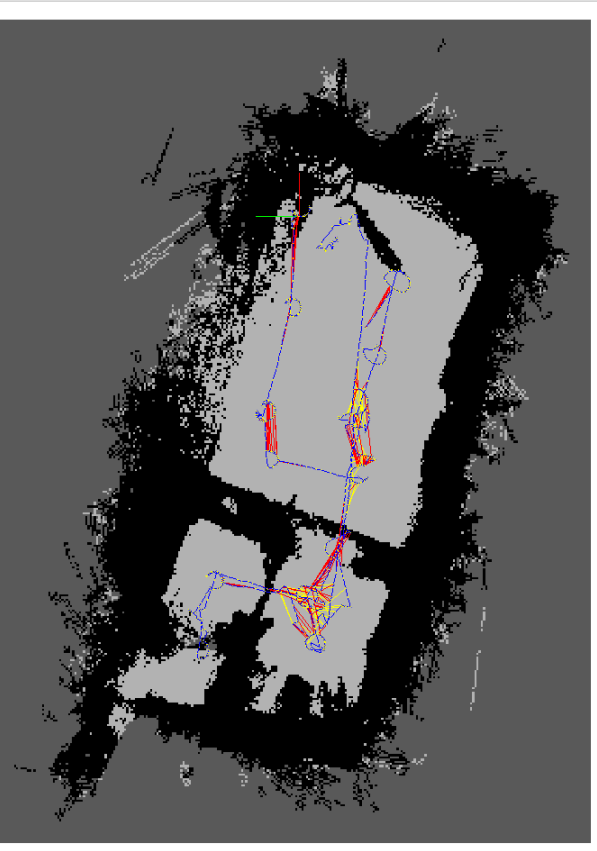
\includegraphics[height=6cm]{Images/mapping graph.png}
    \caption{Mapping Graph}
    \label{fig:mapping_graph}
\end{figure}

\subsubsection{Mapping Mode Implementation}

The mapping mode utilizes the \texttt{rtab\_mapping.launch.py} configuration that enables full SLAM functionality including map building, loop closure detection, and visual feature database creation. The launch file initializes the complete RTABMap pipeline with mapping-optimized parameters.

Key mapping parameters include \texttt{subscribe\_rgbd: True} for synchronized color and depth processing, \texttt{subscribe\_odom\_info: True} for enhanced odometry integration, and \texttt{approx\_sync: False} for precise temporal alignment. The \texttt{wait\_imu\_to\_init: True} parameter ensures proper IMU initialization before beginning mapping operations.

The mapping process operates with continuous loop closure detection and feature database updates. The system maintains visual landmarks and occupancy grid information that supports both immediate navigation and future relocalization. Map visualization through \texttt{rtabmap\_viz} enables real-time monitoring of mapping progress and quality assessment.

\subsubsection{Localization Mode Implementation}

The localization mode utilizes the \texttt{rtab\_localization.launch.py} configuration that loads existing maps and disables new map creation. Critical parameters include \texttt{localization: True} to enable localization-only mode and \texttt{Mem/IncrementalMemory: False} to disable memory updates that would modify the existing map.

The \texttt{Rtabmap/DetectionRate: 3.0} parameter optimizes loop closure detection frequency for localization scenarios, balancing computational load against relocalization performance. The system loads the existing database and continuously tracks robot position within the known map structure.

Relocalization capabilities enable the robot to determine its position within previously created maps even after system restart or temporary tracking loss. The mode supports operation in known environments without requiring new map creation, essential for consistent experimental conditions.

\subsubsection{Mode Switching and Database Management}

The dual-mode architecture enables seamless transitions between mapping and localization operations through launch file selection. Map persistence utilizes the RTABMap database format that maintains visual features, loop closures, and occupancy grids across operational sessions.

Database management includes map saving and loading protocols that ensure data integrity during mode transitions. The system supports multiple map databases for different operational environments, enabling deployment across various research locations without map conflicts.

\subsection{Initial SLAM-Only System Limitations and Drift Issues}

Initial testing of the pure RTABMap implementation revealed significant limitations that necessitated the development of the hybrid sensor fusion approach. Comprehensive testing documented systematic failures that compromised localization accuracy during extended operation.

\subsubsection{Drift Accumulation Analysis}

Extended operation testing revealed position drift accumulation reaching up to 1.2 meters during 30-minute operational sessions. The drift manifested as gradual position error accumulation that increased monotonically with operation time, particularly during movements in feature-poor environments or areas with repetitive visual patterns.

Error source analysis identified visual odometry drift as the primary contributor, exacerbated by lighting changes, motion blur during movement, and insufficient visual features near walls and uniform surfaces. The accumulation proved particularly problematic for VR applications requiring precise robot positioning for immersive interaction.

Statistical analysis of position errors demonstrated systematic bias in specific movement directions, indicating calibration issues and environmental factors affecting feature detection consistency. The four-position testing protocol revealed repeatability issues with standard deviations exceeding 40cm for identical positioning commands.

\subsubsection{Relocalization Challenges}

RTABMap relocalization failures occurred frequently in environments with insufficient distinctive features, requiring manual intervention through robot rotation to achieve sufficient visual feature matching. Feature-poor environments near walls or in corners consistently caused tracking loss, necessitating operator intervention to restore localization.

Map corruption events required complete database reconstruction when loop closure detection failed catastrophically. These failures typically occurred during rapid movement or in areas with dynamic lighting conditions, compromising the entire mapping session and requiring restart from known positions.

The relocalization process proved unreliable for autonomous operation, as successful position recovery often required specific robot orientations and environmental conditions that could not be guaranteed during normal social interaction scenarios.

\subsection{UWB Positioning System Implementation}

The Ultra-Wideband positioning system provides absolute position reference to complement visual SLAM, addressing the drift and relocalization limitations identified in pure SLAM operation. The UWB integration utilizes a third-party positioning package that interfaces with DecaWave hardware through serial communication.

\subsubsection{Hardware Configuration and Integration}

The UWB system utilizes the \texttt{uwb\_positioning} package configured through the \texttt{uwb.launch.py} file. The launch configuration specifies serial communication parameters including \texttt{serial\_port\_name: /dev/ttyACM0} and \texttt{serial\_baud\_rate: 115200} for interface with the UWB hardware module.

The UWB tag integrates directly with the Tino robot platform with minimal interference to other systems. Anchor placement follows a strategic configuration that ensures optimal coverage of the operational environment while minimizing Non-Line-of-Sight (NLOS) conditions that degrade positioning accuracy.

The system publishes absolute position data on the \texttt{/UWB/Pos} topic using \texttt{geometry\_msgs/Pose} message format, providing 3D coordinates that serve as the absolute reference for sensor fusion algorithms.

\subsubsection{Positioning Algorithm and Performance}

The UWB system implements multilateration techniques that calculate 3D position from time-of-flight measurements to multiple anchor points. The positioning algorithm includes NLOS mitigation strategies and noise filtering to provide stable position estimates under typical indoor operational conditions.

Real-time performance characteristics include update rates suitable for robot control applications with latency measurements demonstrating compatibility with real-time system requirements. Accuracy evaluation shows centimeter-level precision under optimal conditions, with graceful degradation in challenging RF environments.

\subsection{Sensor Fusion Between RTABMap Orientation and UWB Positioning}

The hybrid localization system implements sophisticated sensor fusion that combines the complementary strengths of visual SLAM and UWB positioning. The fusion approach separates position and orientation estimation, utilizing UWB for absolute position reference while maintaining RTABMap for orientation data.

\subsubsection{Fusion Algorithm Implementation}

The sensor fusion implementation in the robot controller node utilizes a practical approach that combines UWB absolute positioning with RTABMap orientation data. The \texttt{\_create\_fused\_pose} method implements the core fusion logic that creates unified pose estimates from multiple sensor inputs.

The fusion algorithm prioritizes UWB position data when available, falling back to RTABMap position estimates only when UWB communication fails. Position data from UWB undergoes coordinate frame transformation to align with the RTABMap reference frame, utilizing a configurable 11.5-degree rotation correction applied through the \texttt{\_apply\_rotation\_to\_pose} method.

Orientation estimation maintains RTABMap quaternion data as the primary source, implementing sophisticated validation to detect orientation loss conditions. The system monitors for specific quaternion values (x=1.0, y=0.0, z=0.0, w=0.0) that indicate RTABMap odometry failure and automatically triggers recovery procedures.

\subsubsection{Orientation Loss Detection and Recovery}

The implementation includes robust orientation loss detection that monitors RTABMap output for invalid quaternion values indicating system failure. Upon detection of orientation loss, the system automatically triggers the \texttt{/reset\_odom} service to restart RTABMap odometry while maintaining position tracking through UWB data.

Fallback orientation estimation utilizes movement direction analysis when RTABMap orientation becomes unreliable. The \texttt{\_estimate\_orientation\_from\_movement} method calculates orientation from position history, maintaining operational capability during RTABMap recovery periods. The system stores the last 5 position measurements to enable orientation estimation with minimum 5cm movement thresholds.

Recovery validation continuously monitors RTABMap orientation data to detect system recovery. Upon detection of valid orientation values, the system automatically transitions back to RTABMap orientation while maintaining UWB position data, ensuring seamless operation without manual intervention.

\subsubsection{Coordinate System Alignment}

The sensor fusion system implements coordinate transformation procedures that align UWB coordinates with the SLAM coordinate frame. The transformation includes rotational alignment through quaternion multiplication that corrects for installation and calibration differences between sensor coordinate systems.

The robot controller implements dynamic coordinate frame management that handles different reference frames from various sensors. Position data undergoes proper transformation from \texttt{oak\_right\_camera\_optical\_frame} for camera-based detections while maintaining consistency with UWB absolute coordinates.

Calibration protocols enable adjustment of the coordinate alignment parameters without system modification. The 11.5-degree rotation correction represents empirically determined alignment that ensures consistent positioning across different operational scenarios and environmental conditions.

\subsubsection{Performance Monitoring and Diagnostics}

The fusion system implements comprehensive performance monitoring that tracks sensor health, fusion quality, and system reliability. The robot controller node maintains detailed statistics on UWB availability, RTABMap orientation validity, and fusion algorithm performance.

Communication health monitoring tracks message rates from both UWB and RTABMap systems, providing immediate notification of sensor failures or communication problems. The system logs fusion status information including orientation source selection (RTABMap, movement estimation, or fallback) and position source preference (UWB or RTABMap).

Diagnostic capabilities include real-time logging of sensor fusion decisions, position accuracy validation through movement consistency checking, and comprehensive error reporting that enables rapid identification of localization issues during operation. The monitoring system provides configurable logging levels to balance debugging information with system performance.


\section{Kinematic Base Upgrade from Omnidirectional to Differential Drive}

The kinematic base redesign represents a fundamental shift from the problematic omnidirectional Triksta system to a robust differential drive architecture that addresses the mechanical limitations identified during extended operational testing.

\subsection{Original System Limitations and Failure Analysis}

The original omnidirectional base system utilizing the Triksta platform exhibited systematic failures under the operational demands of the 20kg Tino robot. Comprehensive analysis revealed multiple failure modes that compromised system reliability and operational capability.

\begin{figure}[H]
    \centering
    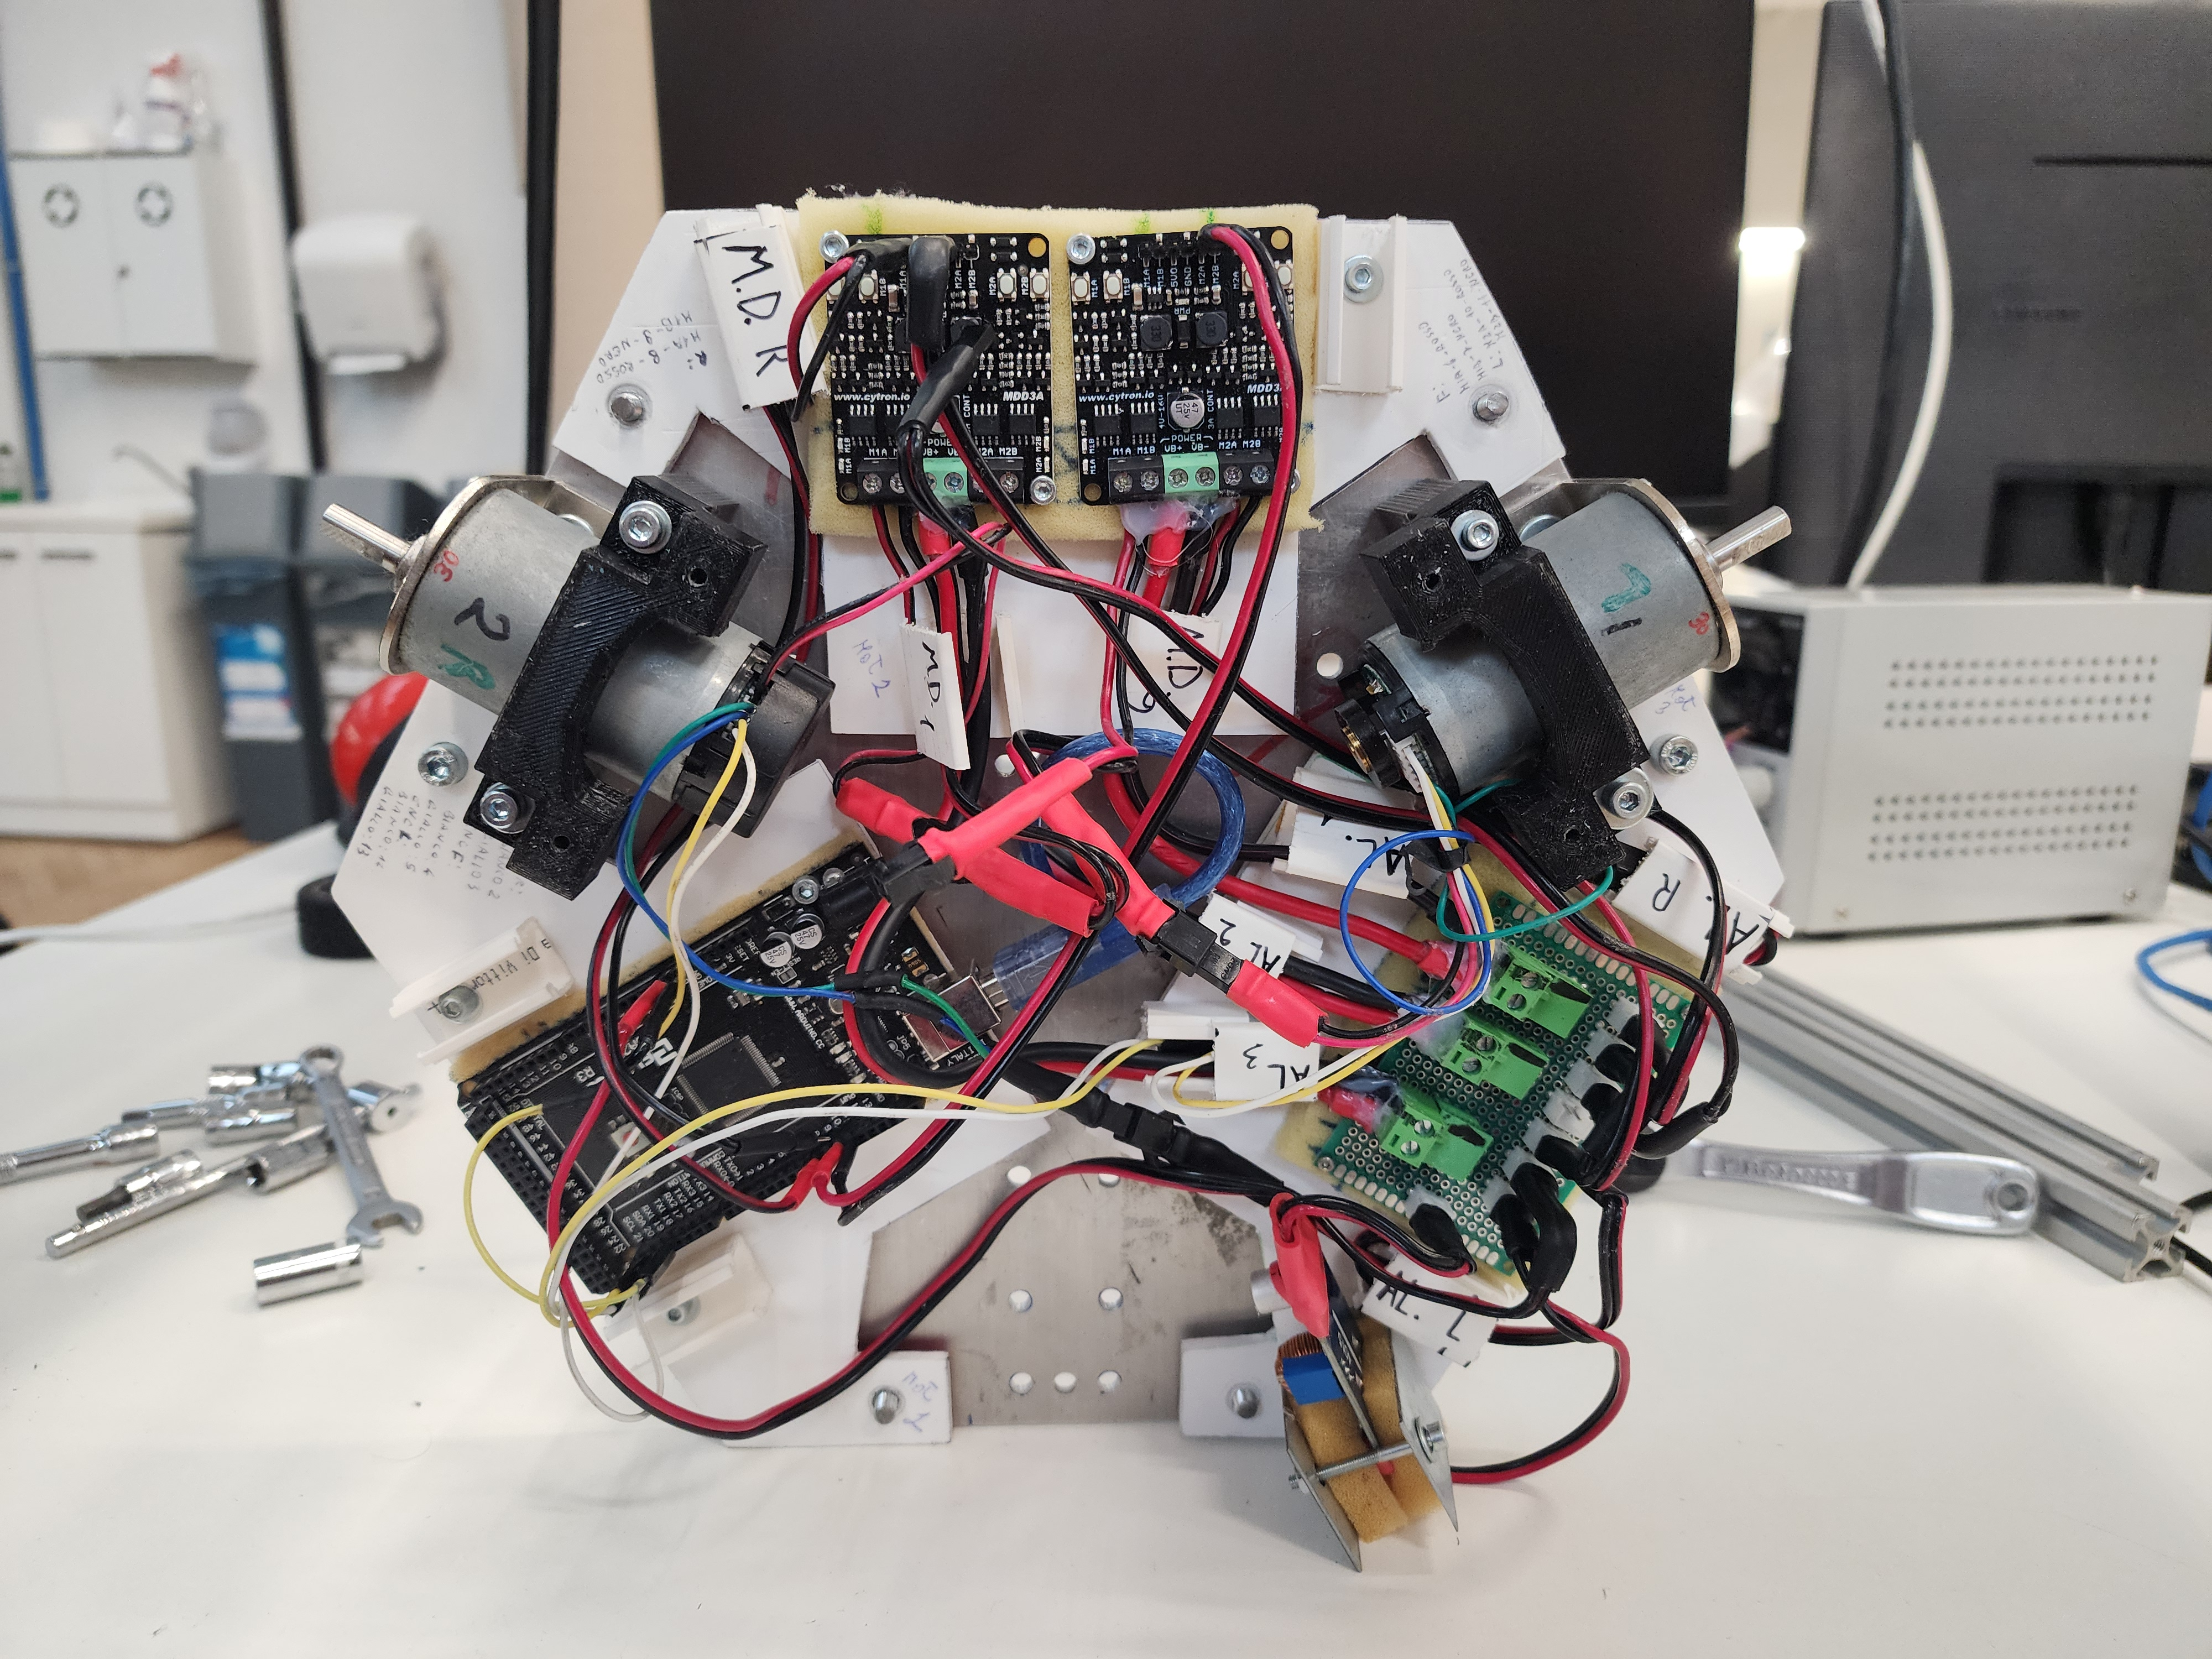
\includegraphics[width=0.8\textwidth]{Images/OriginalTrikstaBase.jpg}
    \caption{Original Triksta Base System}
    \label{fig:original_triksta_base}
\end{figure}

\subsubsection{Omniwheel Mechanical Failures}

The omniwheel rollers experienced systematic deformation under Tino's 20kg operational weight, with roller surfaces becoming squared due to continuous plastic deformation. This deformation created irregular rolling characteristics that manifested as vibration, reduced traction, and unpredictable movement behavior during social interaction scenarios.

Roller bearing failures occurred frequently in the rear omniwheel due to the dragging forces encountered during forward movement and turning operations. The omnidirectional capability proved unnecessary for social robot applications, as Tino's interaction patterns primarily required forward movement with turning capabilities rather than true omnidirectional motion.

Load distribution analysis revealed that the three-wheel configuration created uneven weight distribution with the rear wheel experiencing excessive drag forces. This asymmetric loading accelerated wear patterns and contributed to premature component failure, particularly during sustained operation periods required for social interaction research.

\subsubsection{Motor Performance and Control Challenges}

The original motor configuration struggled to provide consistent torque under the sustained loading conditions required for Tino's operation. Motor heating issues developed during extended use, leading to performance degradation and potential component damage that threatened operational reliability.

Control system complexity increased significantly due to the omnidirectional kinematics, requiring sophisticated coordination between three drive motors while compensating for mechanical variability and wear. The VirHas library dependency created maintenance challenges and limited customization capabilities for the specific requirements of the Tino platform.

\subsection{Differential Drive Architecture Design}

The differential drive architecture selection prioritized mechanical simplicity, enhanced reliability, and improved maintainability while providing adequate maneuverability for social robot applications.

\begin{figure}[H]
    \centering
    \includegraphics[width=0.7\textwidth]{Images/NewBaseDifferentialDrive.jpg}
    \caption{Complete Differential Drive Base with T-Structure Framework}
    \label{fig:differential_base_complete}
\end{figure}

\subsubsection{Kinematic Simplification and Performance Benefits}

The differential drive design eliminates the mechanical complexity of omnidirectional systems while maintaining the essential mobility requirements for social interaction scenarios. The two-wheel configuration with rear caster provides stable platform dynamics with reduced component count and simplified maintenance requirements.

Weight distribution optimization utilizes the two front drive wheels to support the majority of Tino's operational weight while the rear caster wheel provides stability without bearing significant driving loads. This configuration eliminates the dragging forces that compromised the original omnidirectional system.

Maneuverability analysis demonstrates that differential drive provides adequate turning capability for social robot applications through differential wheel speed control. The simplified kinematics enable more precise movement control and improved repeatability compared to the three-wheel omnidirectional system.

\subsection{Mechanical Implementation and Structural Modifications}

The mechanical implementation required comprehensive base modification utilizing aluminum Item profiles to create a robust and adjustable platform architecture.

\subsubsection{T-Structure Construction with Aluminum Profiles}

The T-structure design utilizes aluminum Item profiles to create a dynamic and adjustable framework that enables optimal wheel positioning for weight distribution and traction optimization. The modular profile system provides structural rigidity while allowing mechanical adjustments without complete system redesign.
\begin{figure}[H]
    \centering
    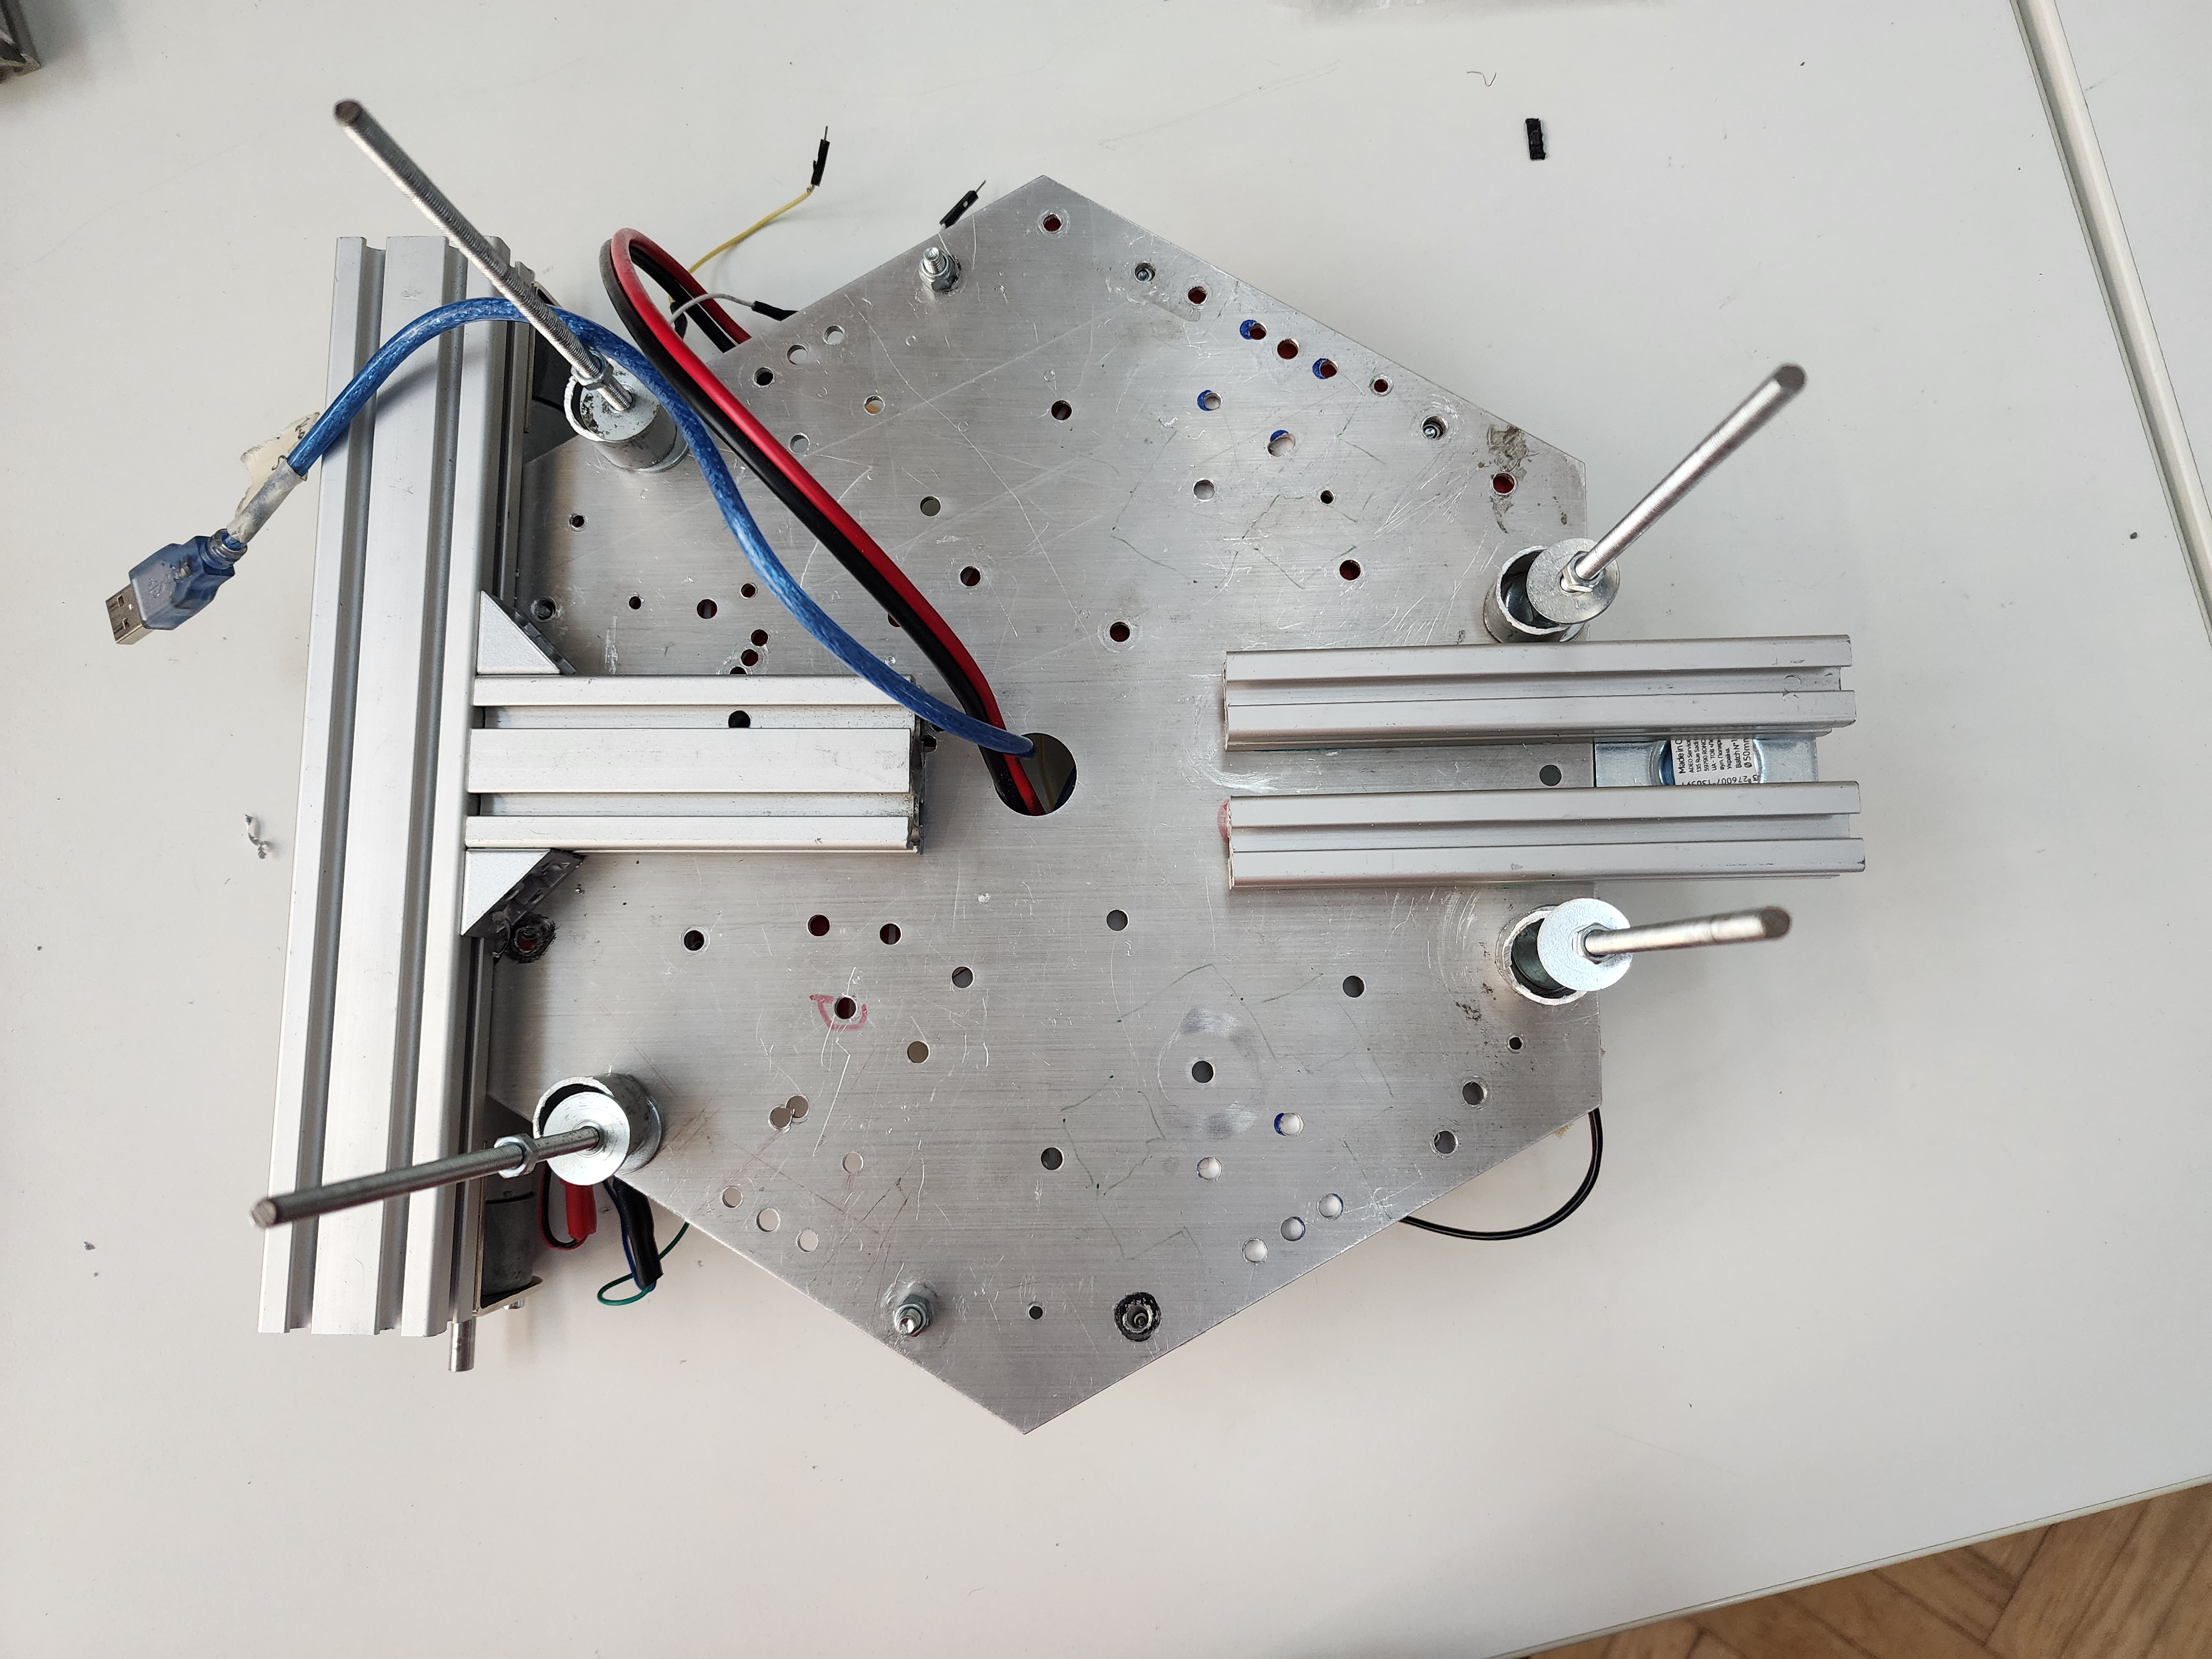
\includegraphics[width=0.6\textwidth]{Images/NewBaseDifferentialDrive (5).jpg}
    \caption{Top View of Differential Drive Base with T-Structure}
    \label{fig:differential_base_top}
\end{figure}
Wheel spacing optimization through the adjustable T-structure enables fine-tuning of track width to achieve proper balance and stability characteristics. The aluminum construction provides excellent strength-to-weight ratio while maintaining the structural integrity required for Tino's operational loads.

\begin{figure}[H]
    \centering
    \begin{minipage}{0.45\textwidth}
        \centering
        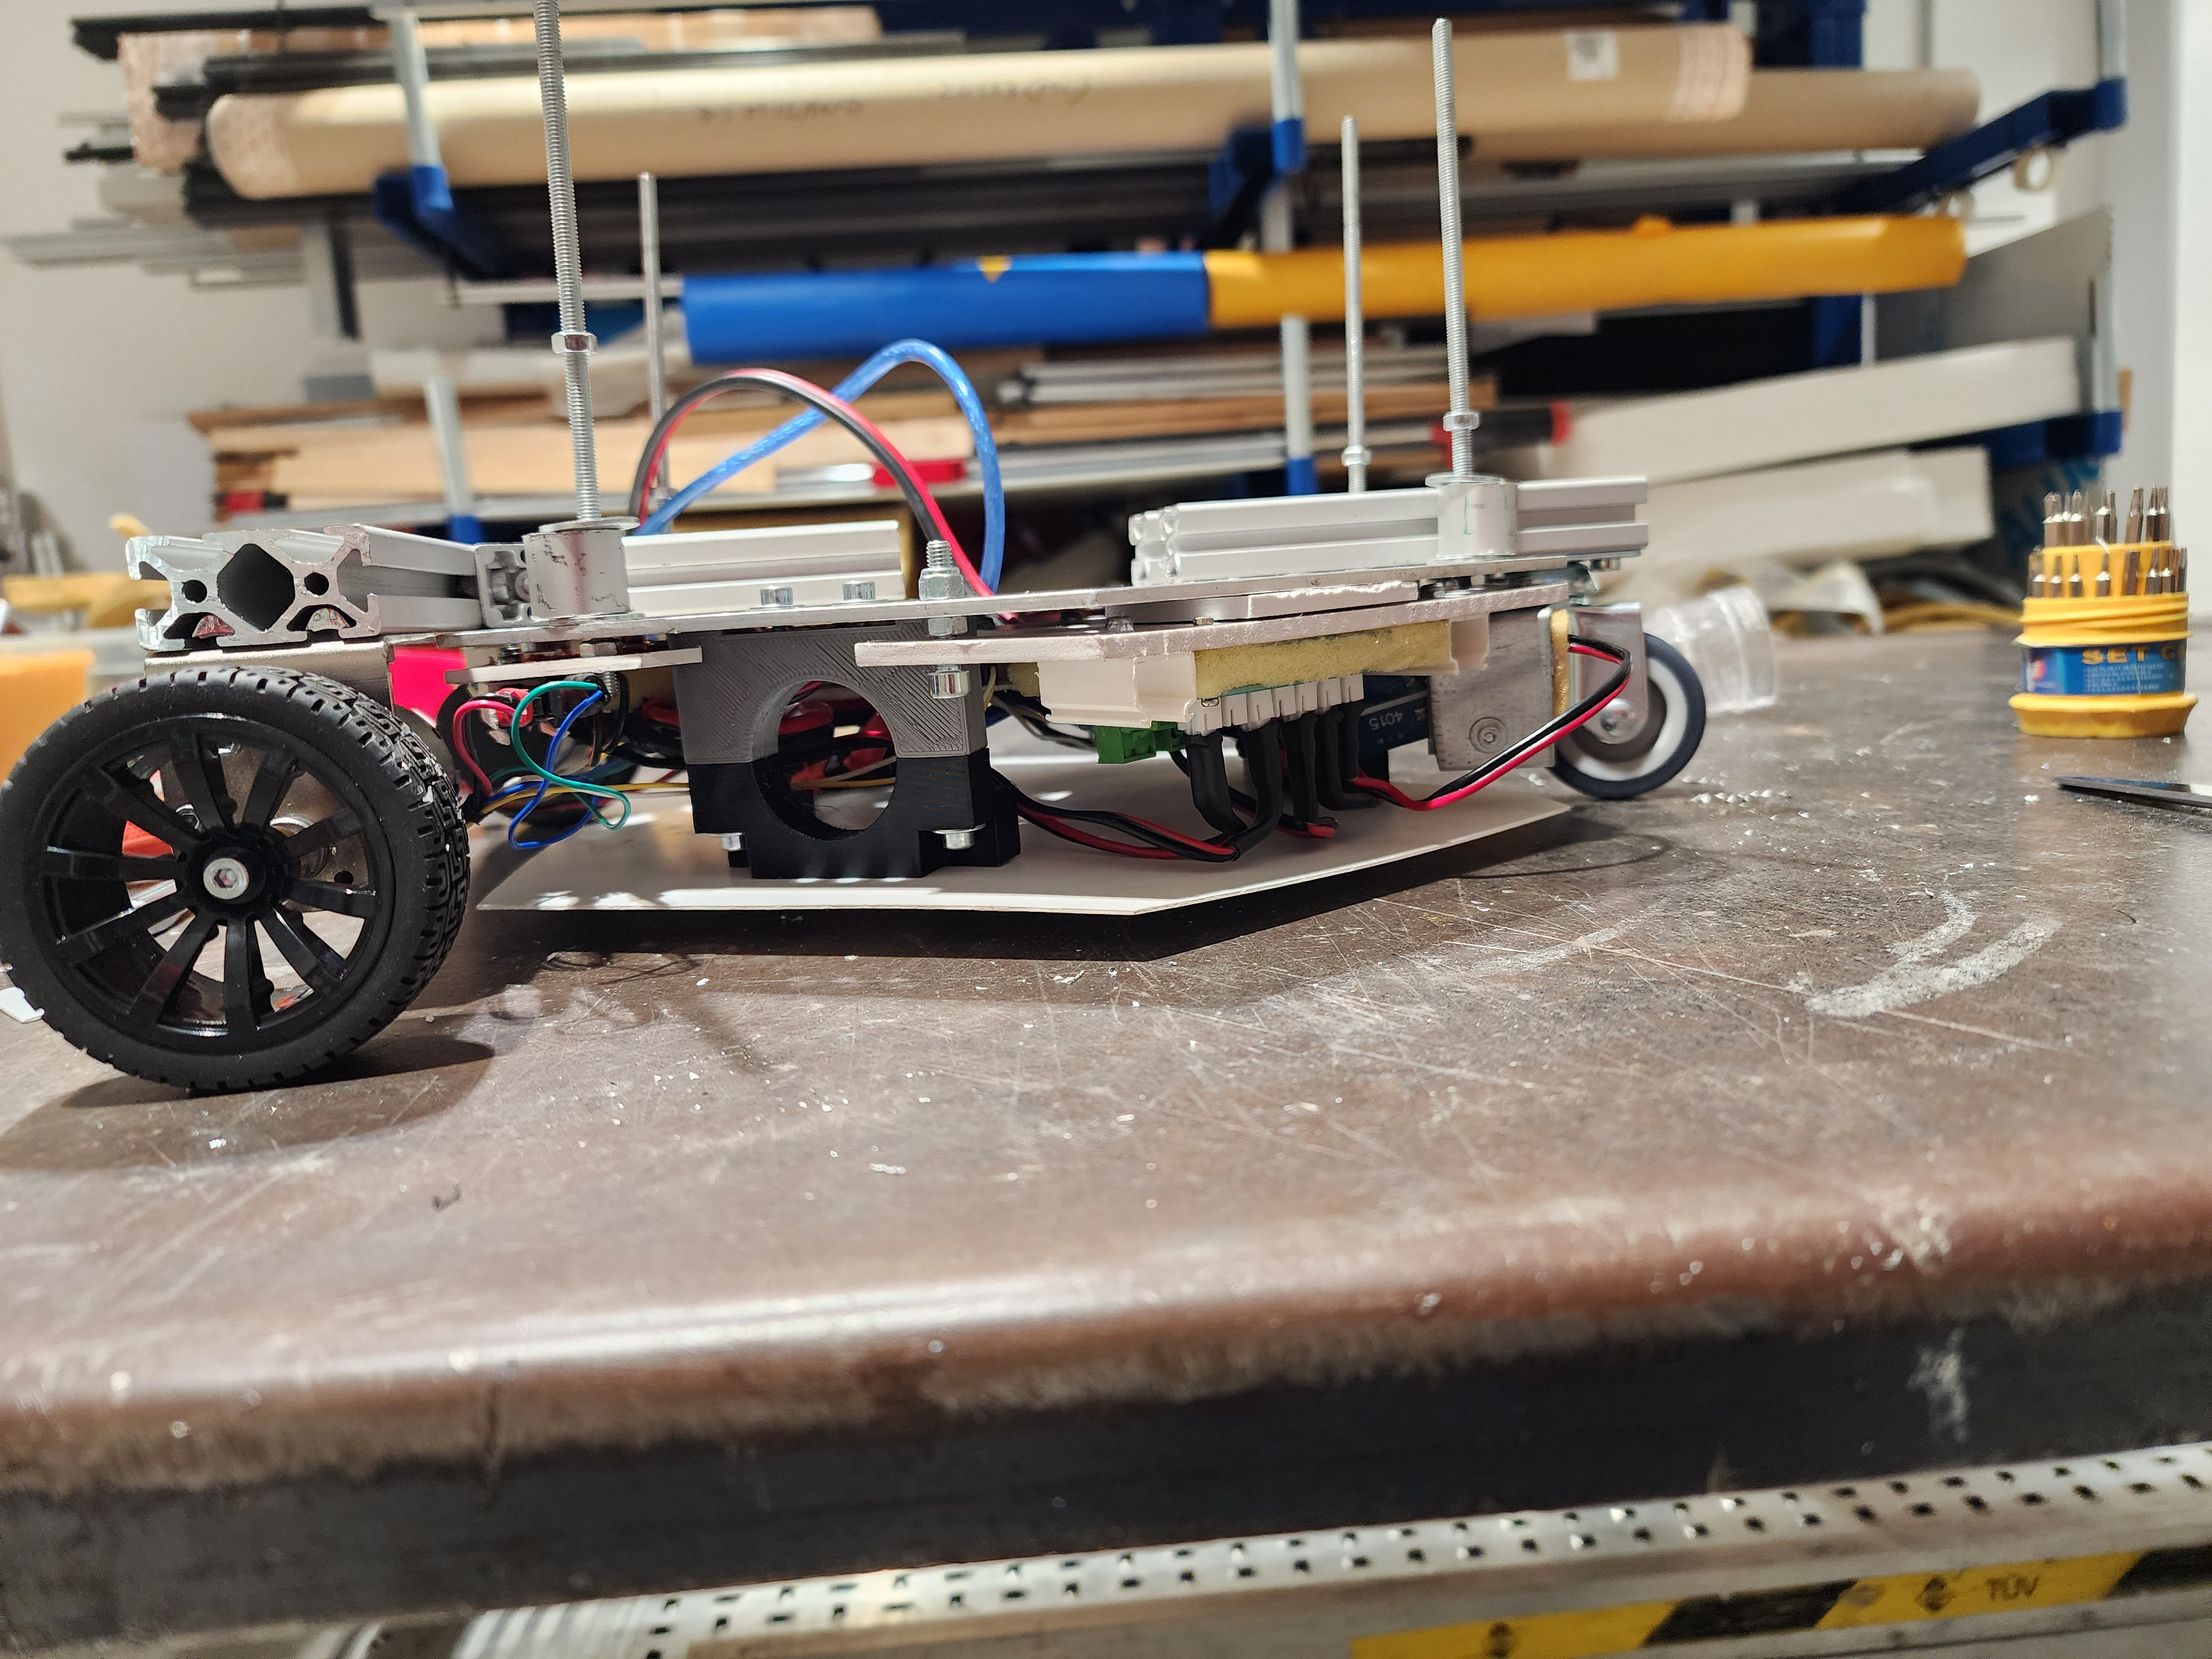
\includegraphics[width=\textwidth]{Images/NewBaseDifferentialDrive (2).jpg}
        \caption{Differential Drive Base Side View}
        \label{fig:differential_base_side}
    \end{minipage}
    \hfill
    \begin{minipage}{0.45\textwidth}
        \centering
        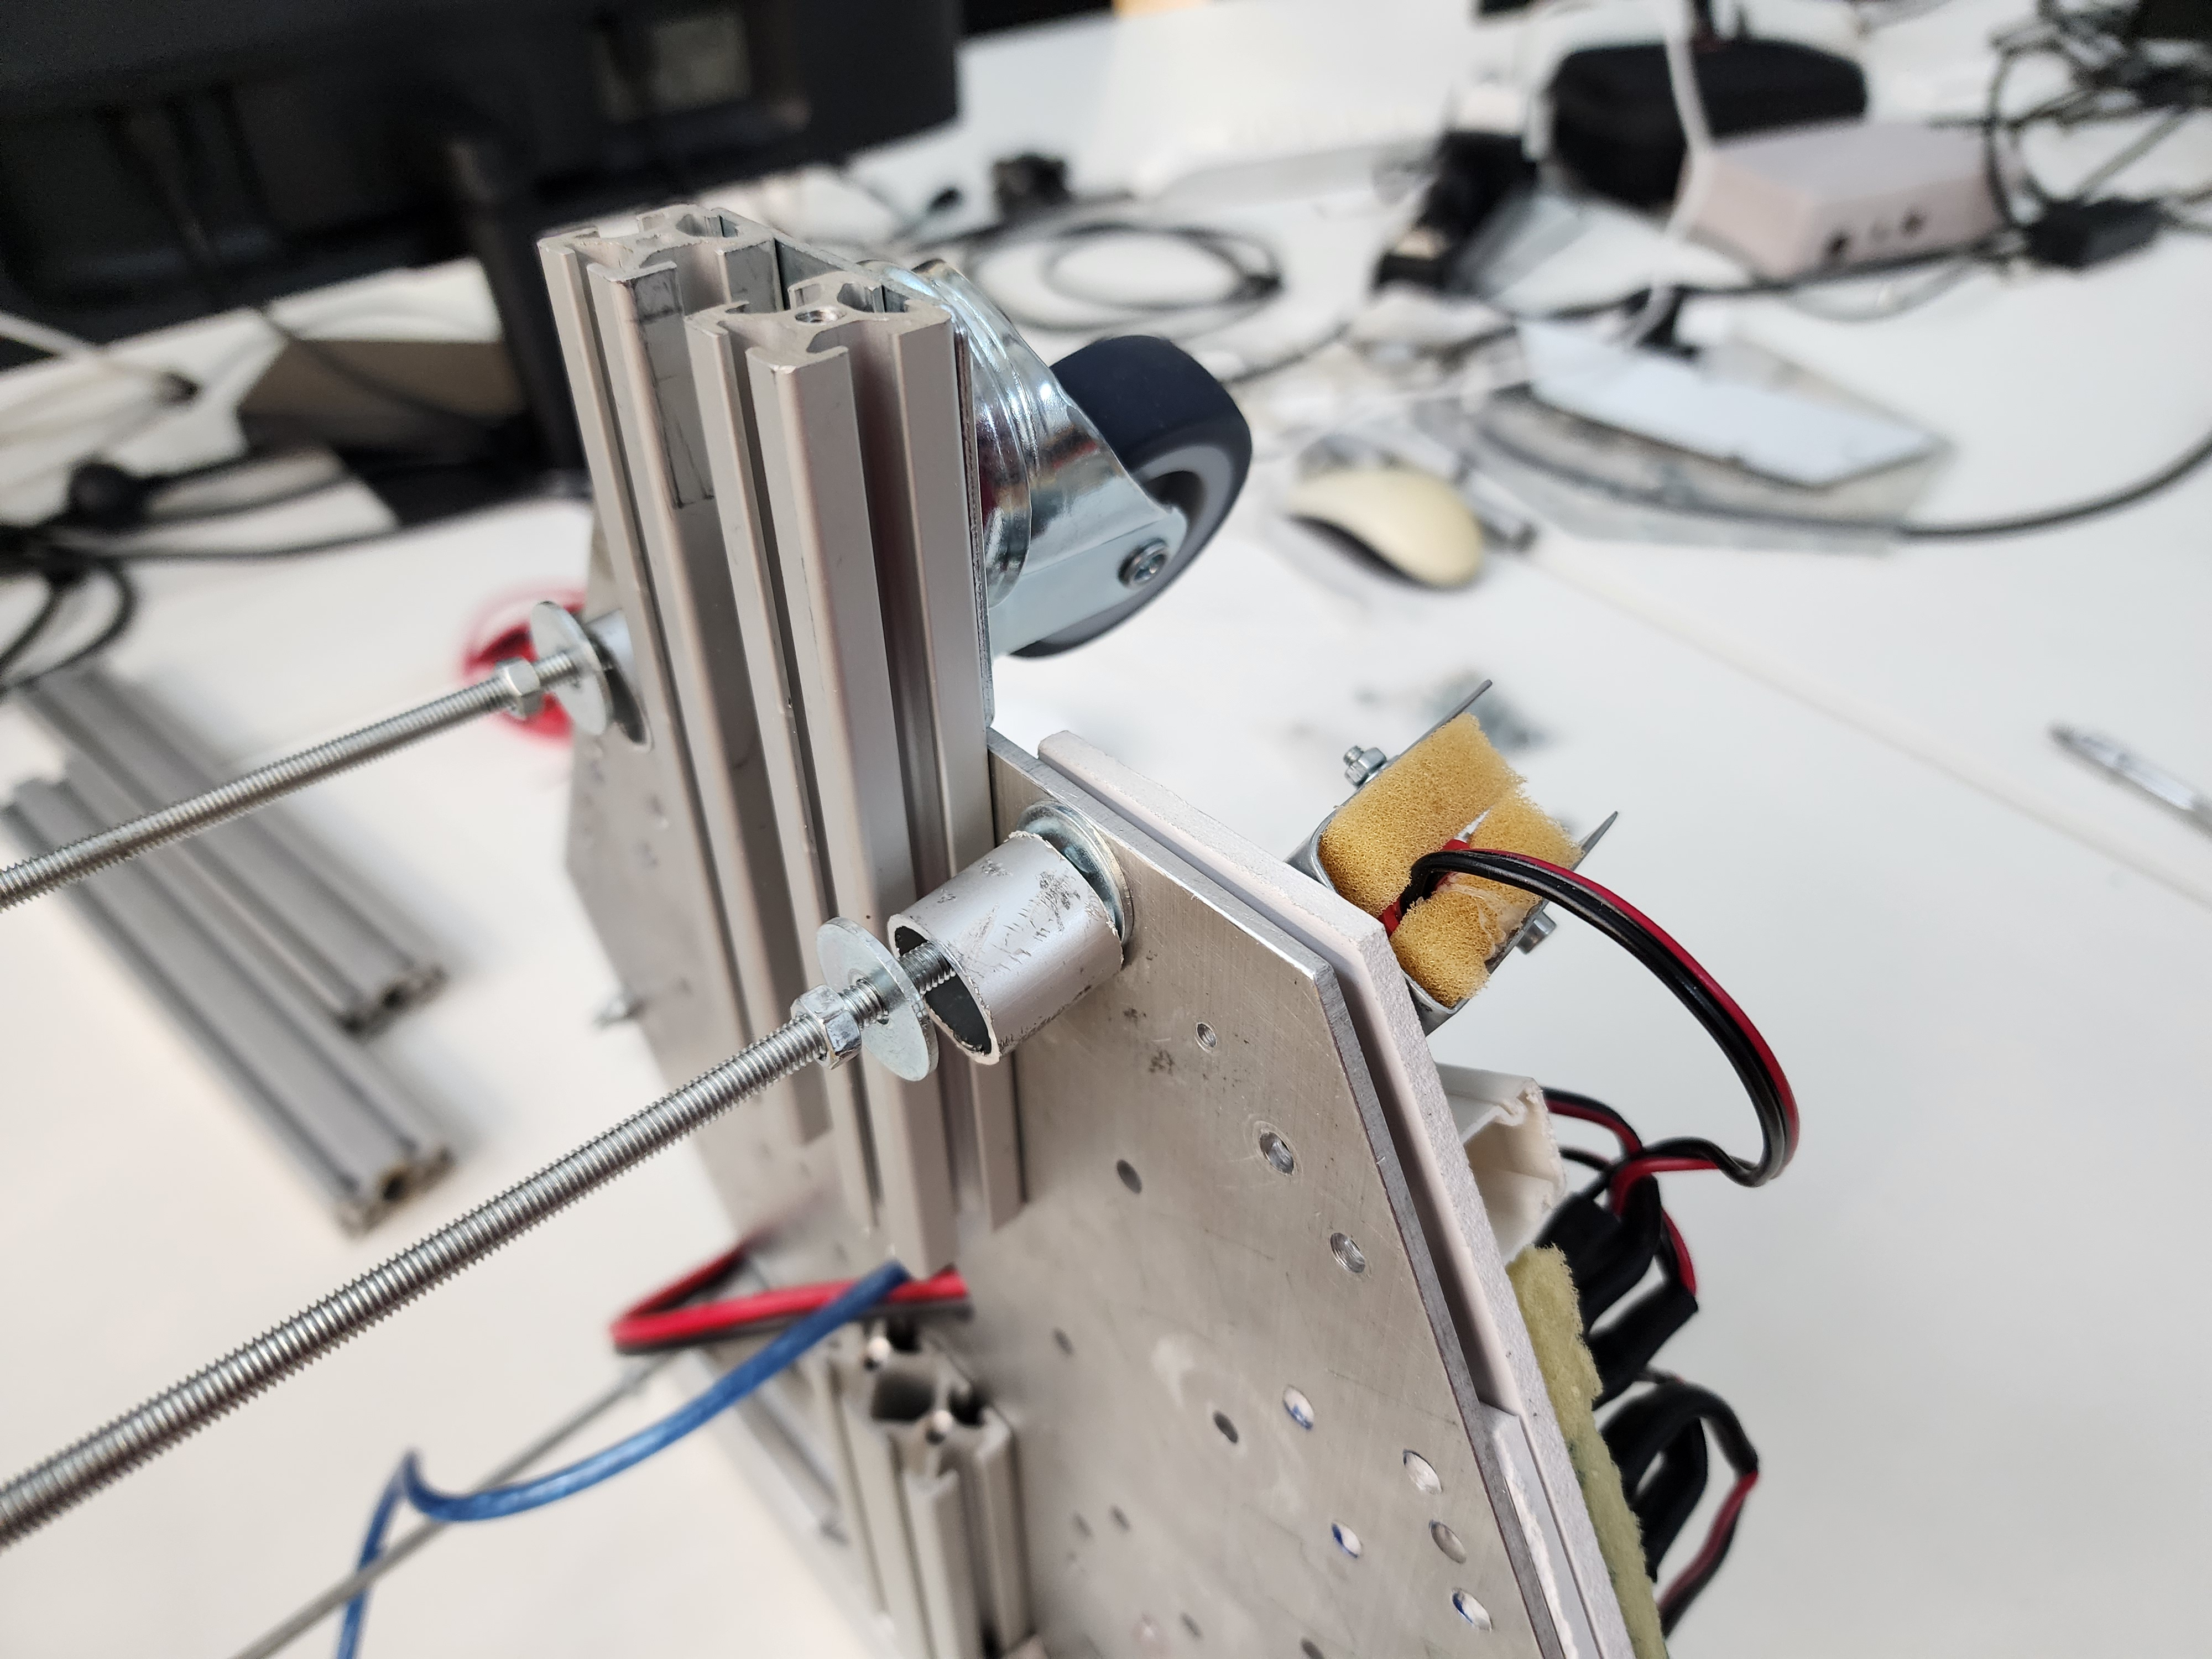
\includegraphics[width=\textwidth]{Images/NewBaseDifferentialDrive (3).jpg}
        \caption{Caster Wheel supporting Rear of Base}
        \label{fig:differential_base_caster}
    \end{minipage}
\end{figure}

Motor mounting points integrate directly with the Item profile system through custom brackets that provide precise motor alignment and secure attachment. The modular design enables motor replacement or upgrade without structural modifications to the base platform.

\subsubsection{Motor Upgrade and Drive System Enhancement}

The motor upgrade to more powerful units addresses the thermal and torque limitations identified in the original system. The new motors provide enhanced heat dissipation capabilities and higher continuous torque ratings suitable for Tino's operational requirements.

\begin{figure}[H]
    \centering
    \begin{minipage}{0.45\textwidth}
        \centering
        \includegraphics[width=\textwidth,angle=-90]{Images/BaseNewMotors.jpg}
        \caption{Base with New Motors (Top View)}
        \label{fig:base_new_motors}
    \end{minipage}
    \hfill
    \begin{minipage}{0.45\textwidth}
        \centering
        \includegraphics[width=\textwidth,angle=-90]{Images/BaseNewMotors2.jpg}
        \caption{Base with New Motors (Close up Side View)}
        \label{fig:base_new_motors_side}
    \end{minipage}
\end{figure}

Motor driver upgrade to the MDD10A units provides increased current handling capability and enhanced control responsiveness compared to the original dual-driver configuration. The single-driver solution simplifies electrical connections while providing superior performance characteristics for differential drive control.

\subsection{Wheel System Development and Traction Solutions}

The wheel selection and mounting system required iterative development to address the unique challenges of supporting Tino's weight while maintaining reliable traction and durability.

\subsubsection{Wheel Selection Evolution and Testing}

Initial wheel selection utilized plastic wheels with pneumatic rubber tires that provided adequate traction but suffered from hub failure under operational loads. The plastic hub construction proved inadequate for the sustained loading conditions, requiring multiple repairs and replacements during system development.

Tire debeading issues occurred when the rubber tire separated from the plastic hub due to inadequate bonding strength under operational stress. Multiple repair approaches were evaluated, including hot-glue reinforcement that provided temporary solutions but required periodic maintenance.

Wheel hub reinforcement through hot-glue filling addressed the structural weakness in the plastic hub construction. This solution proved effective in preventing debeading while maintaining adequate traction characteristics, though it represents a temporary fix requiring future wheel system upgrade.

\begin{figure}[H]
    \centering
    \begin{subfigure}{0.45\textwidth}
        \centering
        \includegraphics[width=\textwidth]{Images/WheelSilicona (3).jpg}
        \caption{Wheel Front View}
        \label{fig:wheel_hotglue}
    \end{subfigure}
    \hfill
    \begin{subfigure}{0.45\textwidth}
        \centering
        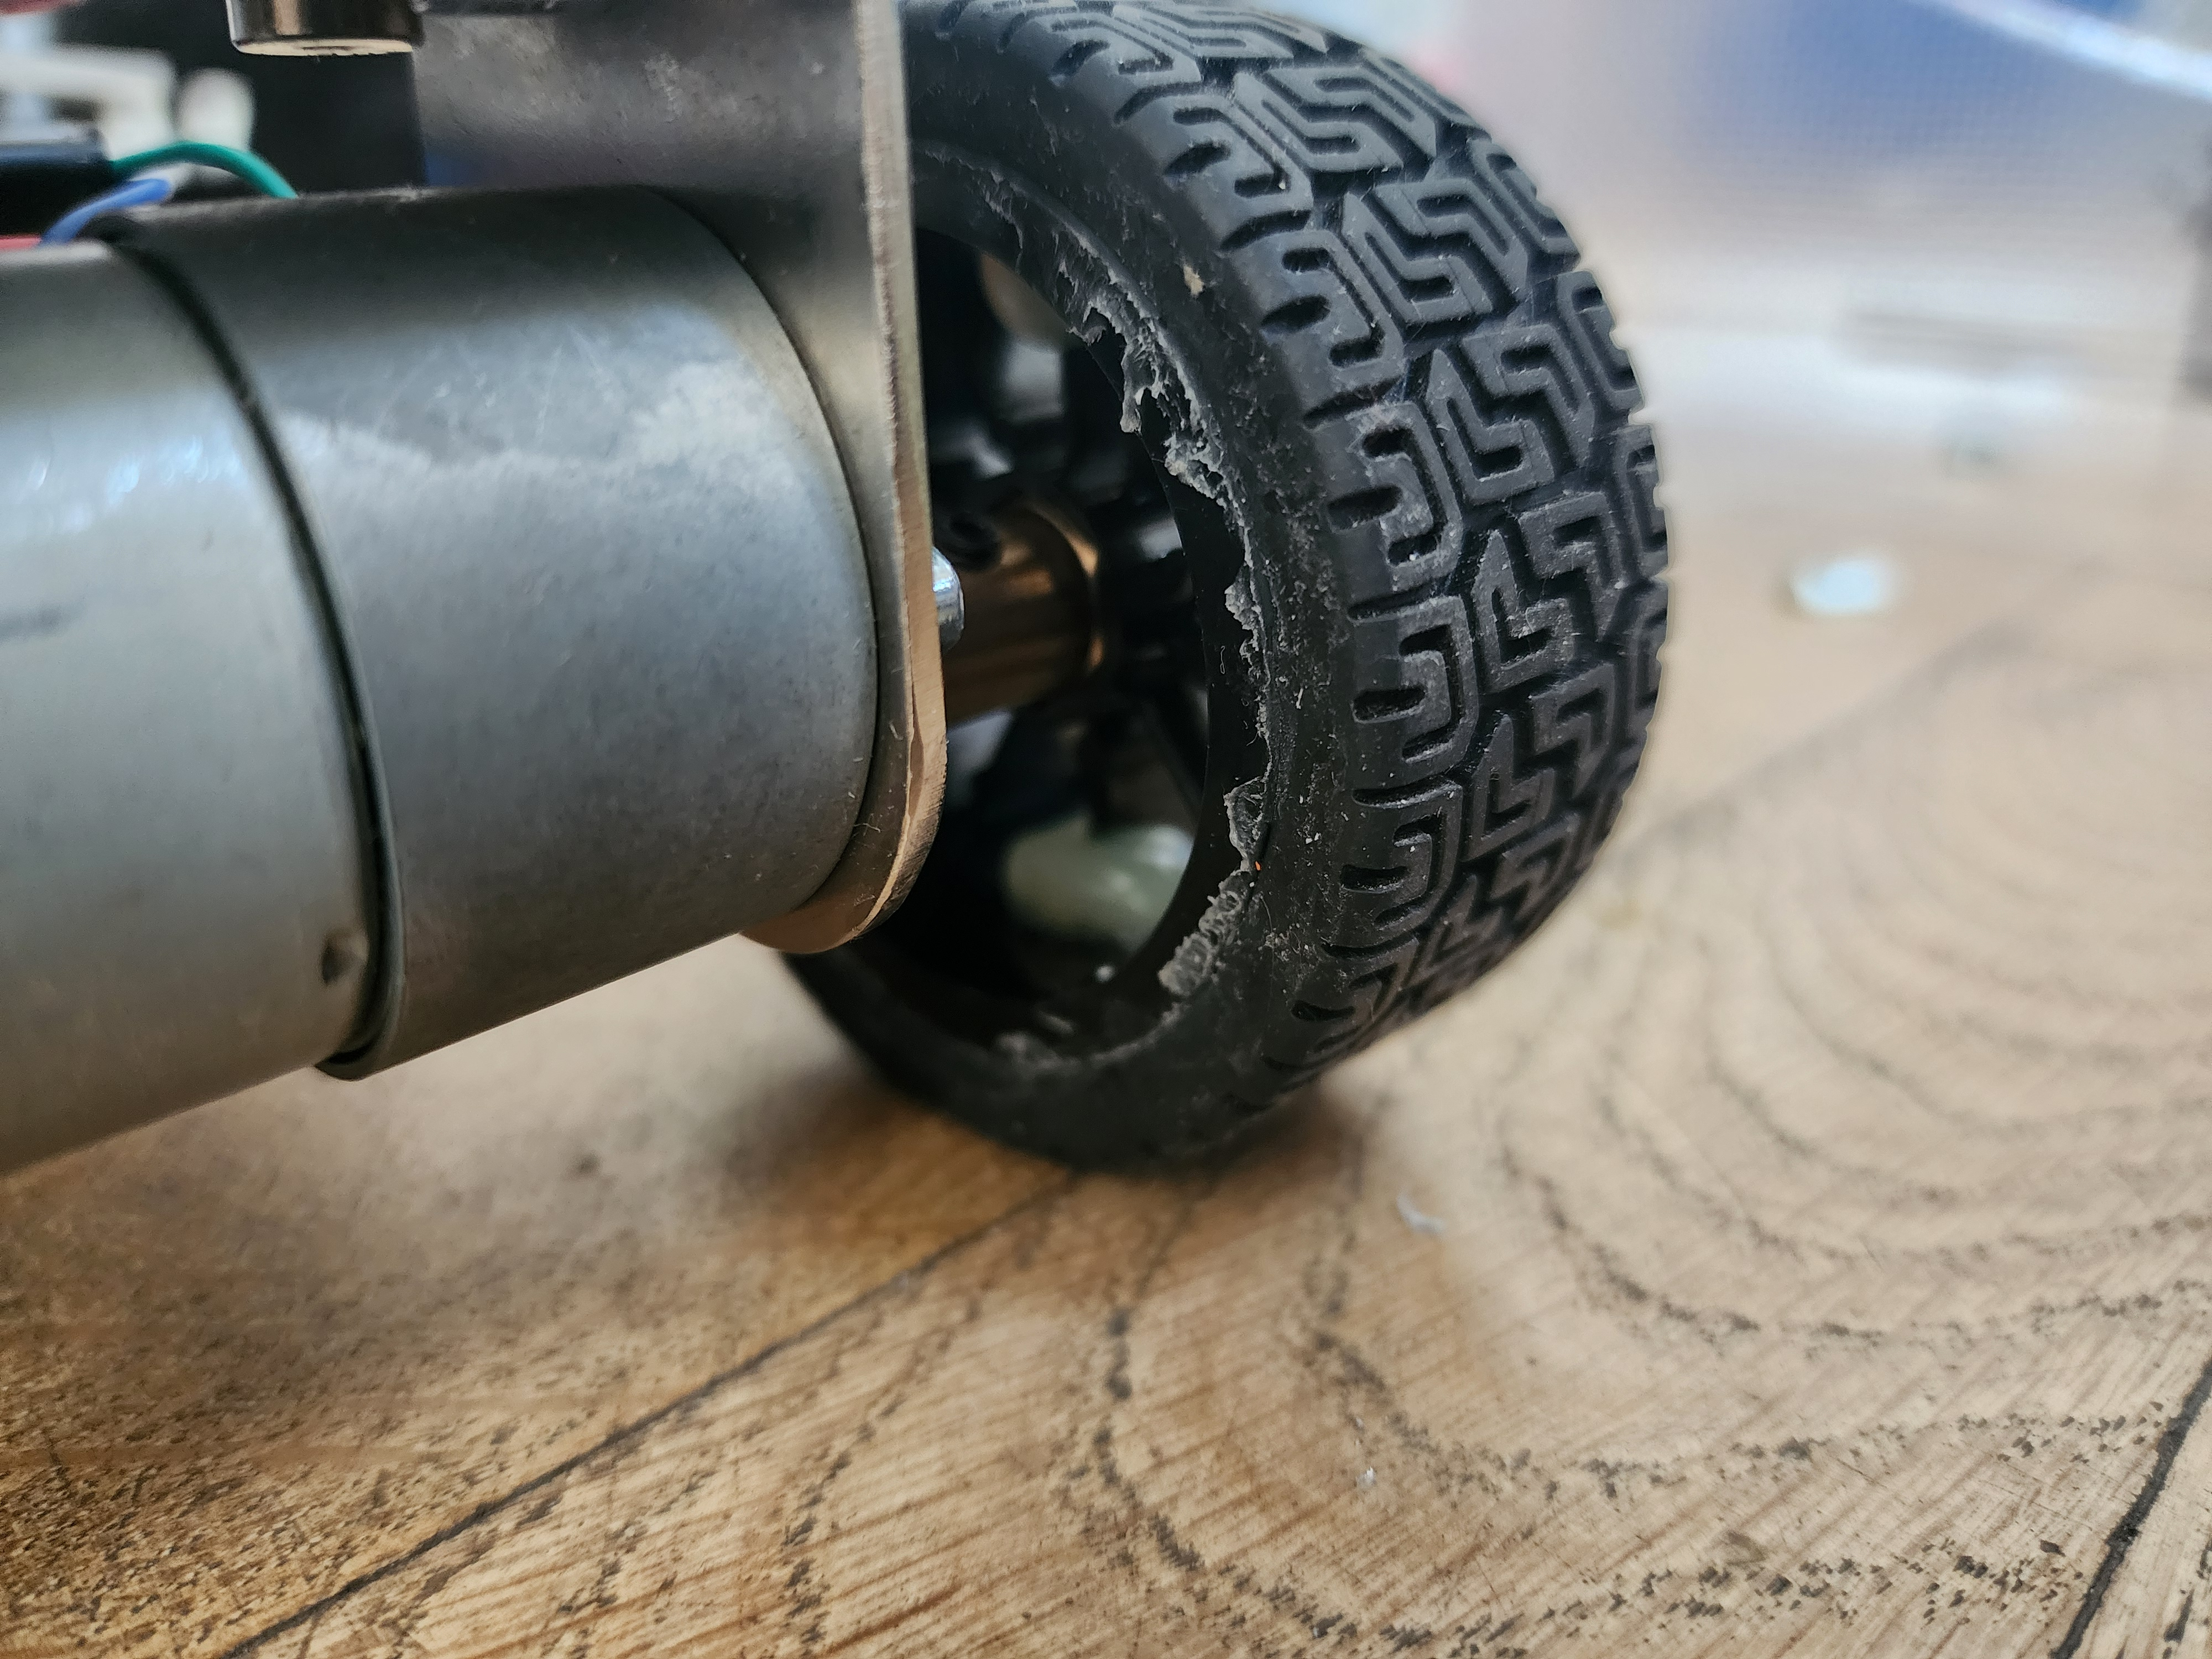
\includegraphics[width=\textwidth]{Images/WheelSilicona.jpg}
        \caption{Wheel Mounted on Motor Shaft}
        \label{fig:wheel_silicone}
    \end{subfigure}
    \caption{Wheel with Hot-Glue Filled Tires}
    \label{fig:combined}
\end{figure}

\subsubsection{Fabric Protection and Bumper Implementation}

Fabric interference prevention required the implementation of protective bumpers to prevent Tino's fabric covering from interfering with wheel operation. The bumper design provides physical separation between the moving wheels and the flexible fabric structure.

\begin{figure}[H]
    \centering
    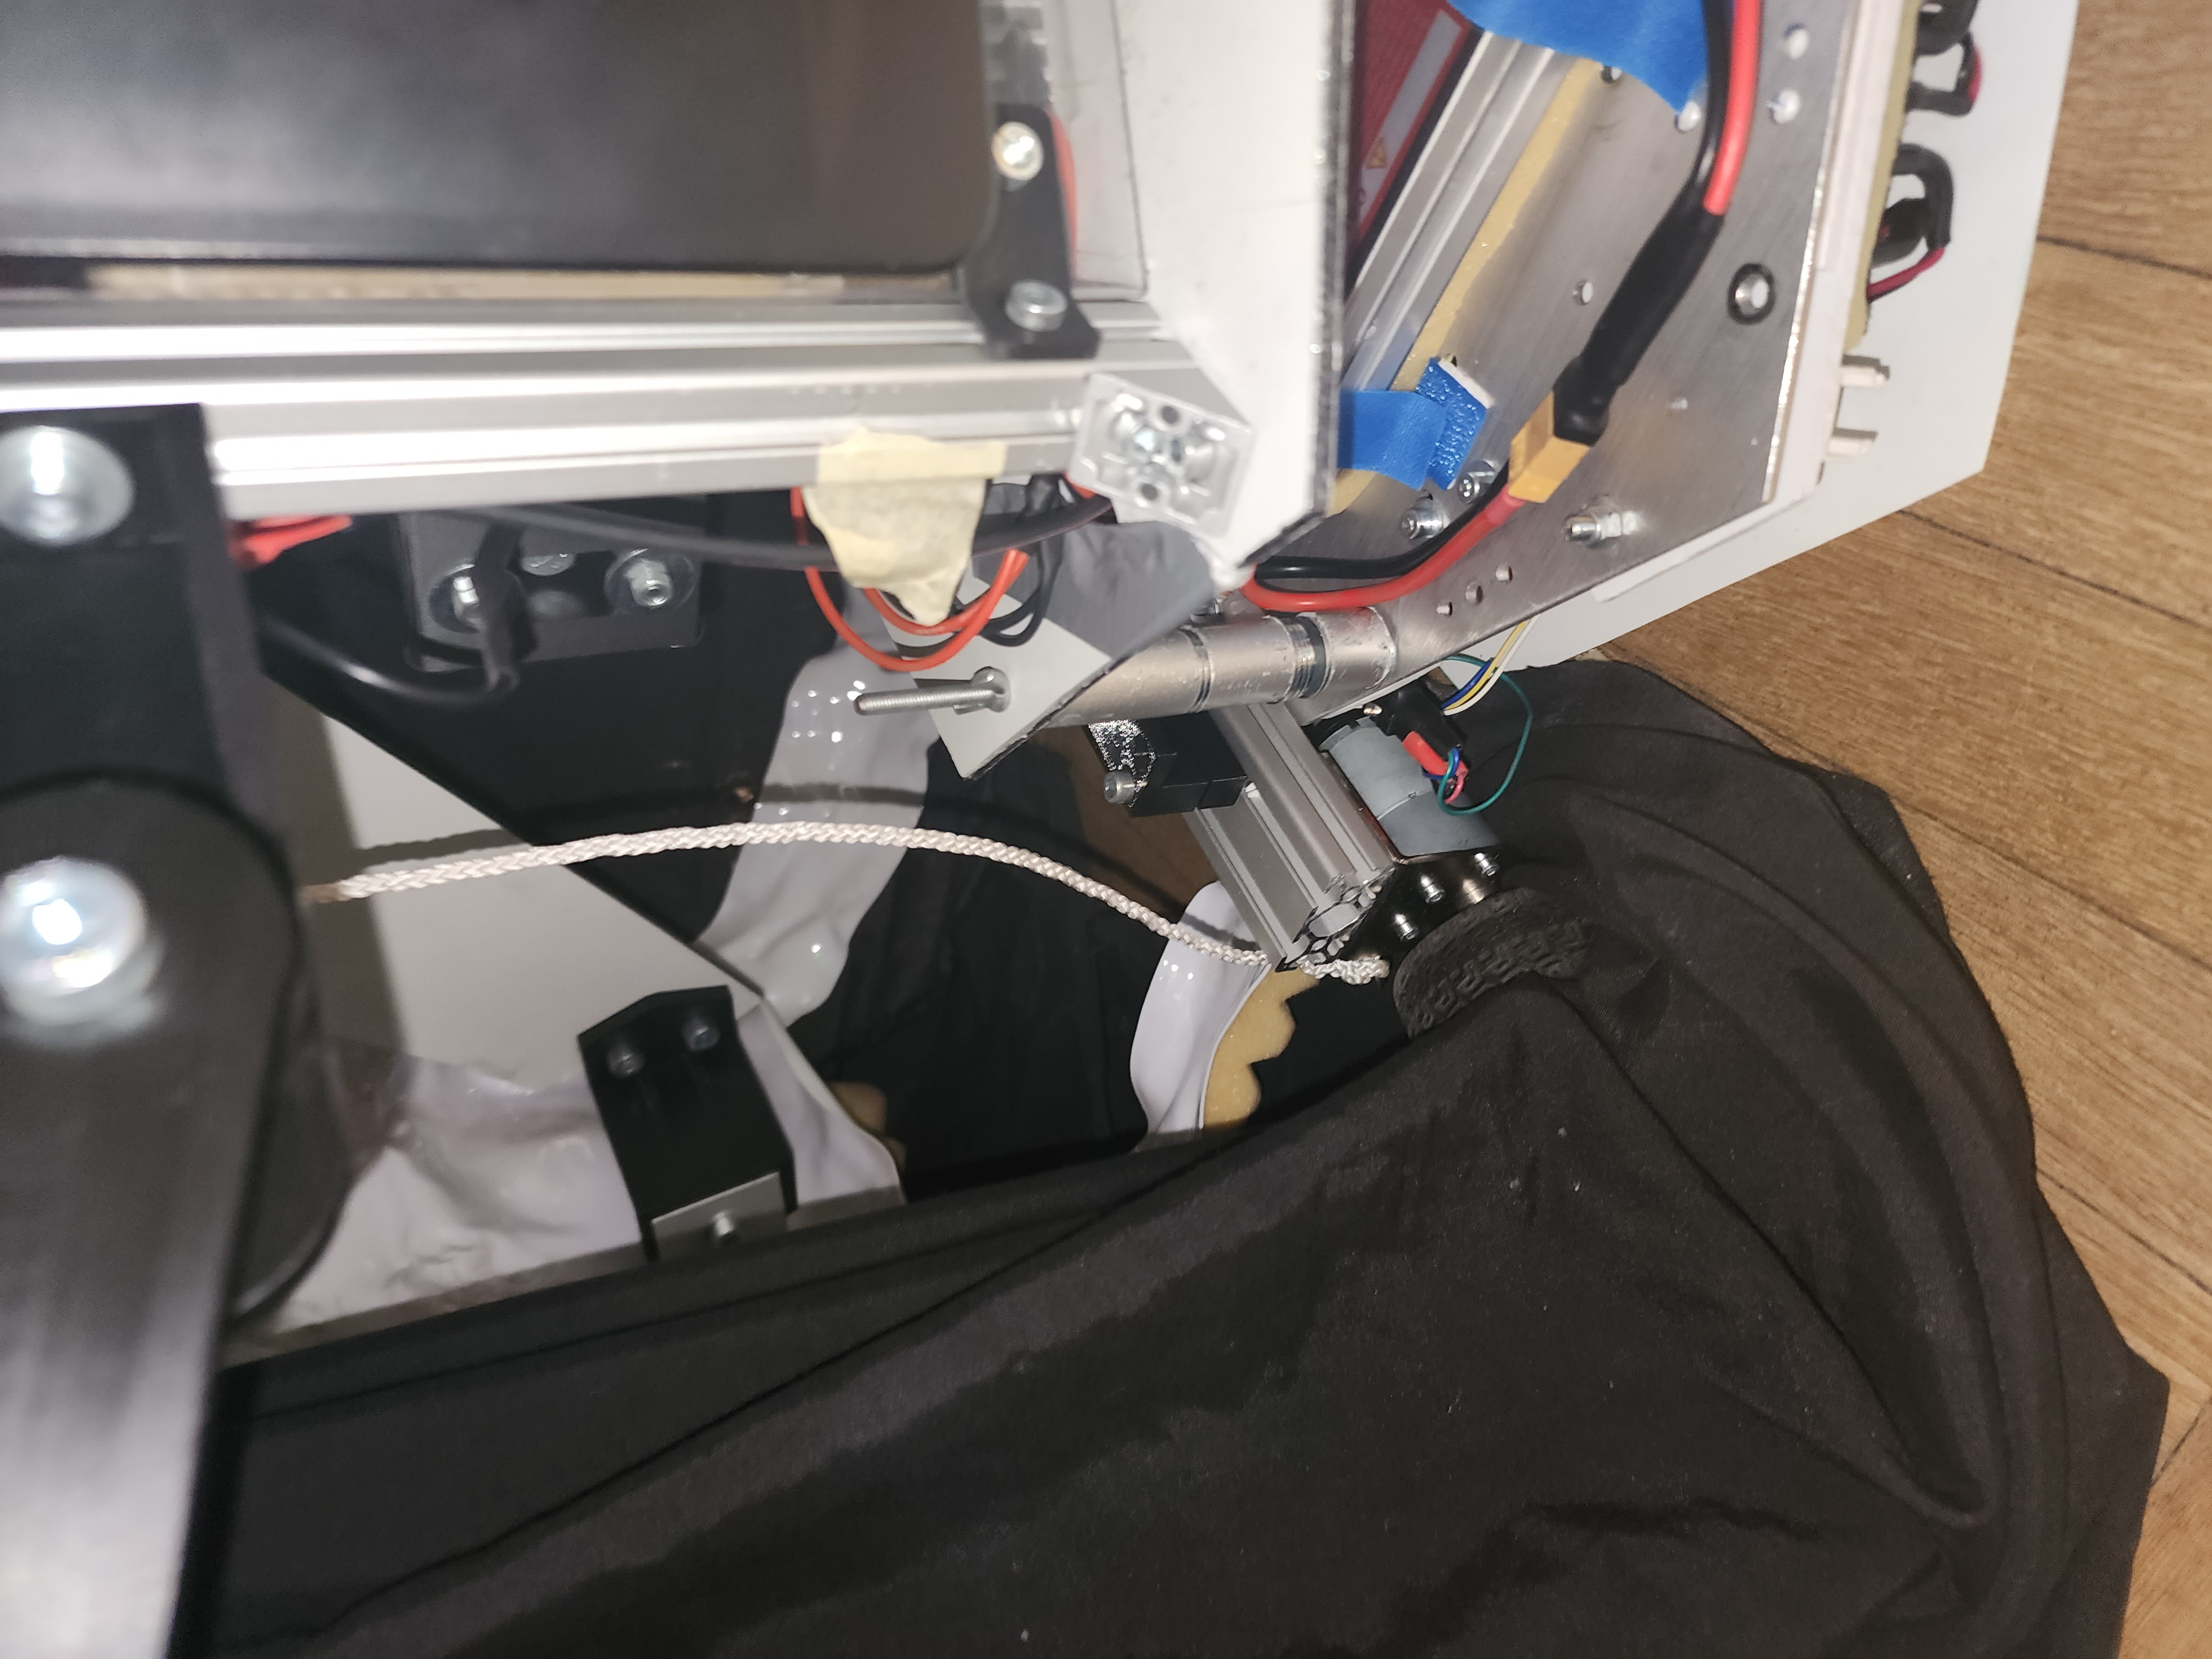
\includegraphics[height=6cm,angle=-90]{Images/WheelVSFabric (2).jpg}
    \caption{Wheel vs Fabric Interference}
    \label{fig:wheel_vs_fabric}
\end{figure}

Bumper effectiveness testing demonstrated successful prevention of fabric entanglement in most operational scenarios, though some edge cases still require operator attention. The bumper system represents a practical solution that addresses the majority of fabric interference issues without compromising Tino's aesthetic design.

\begin{figure}[H]
    \centering
    \begin{minipage}{0.45\textwidth}
        \centering
        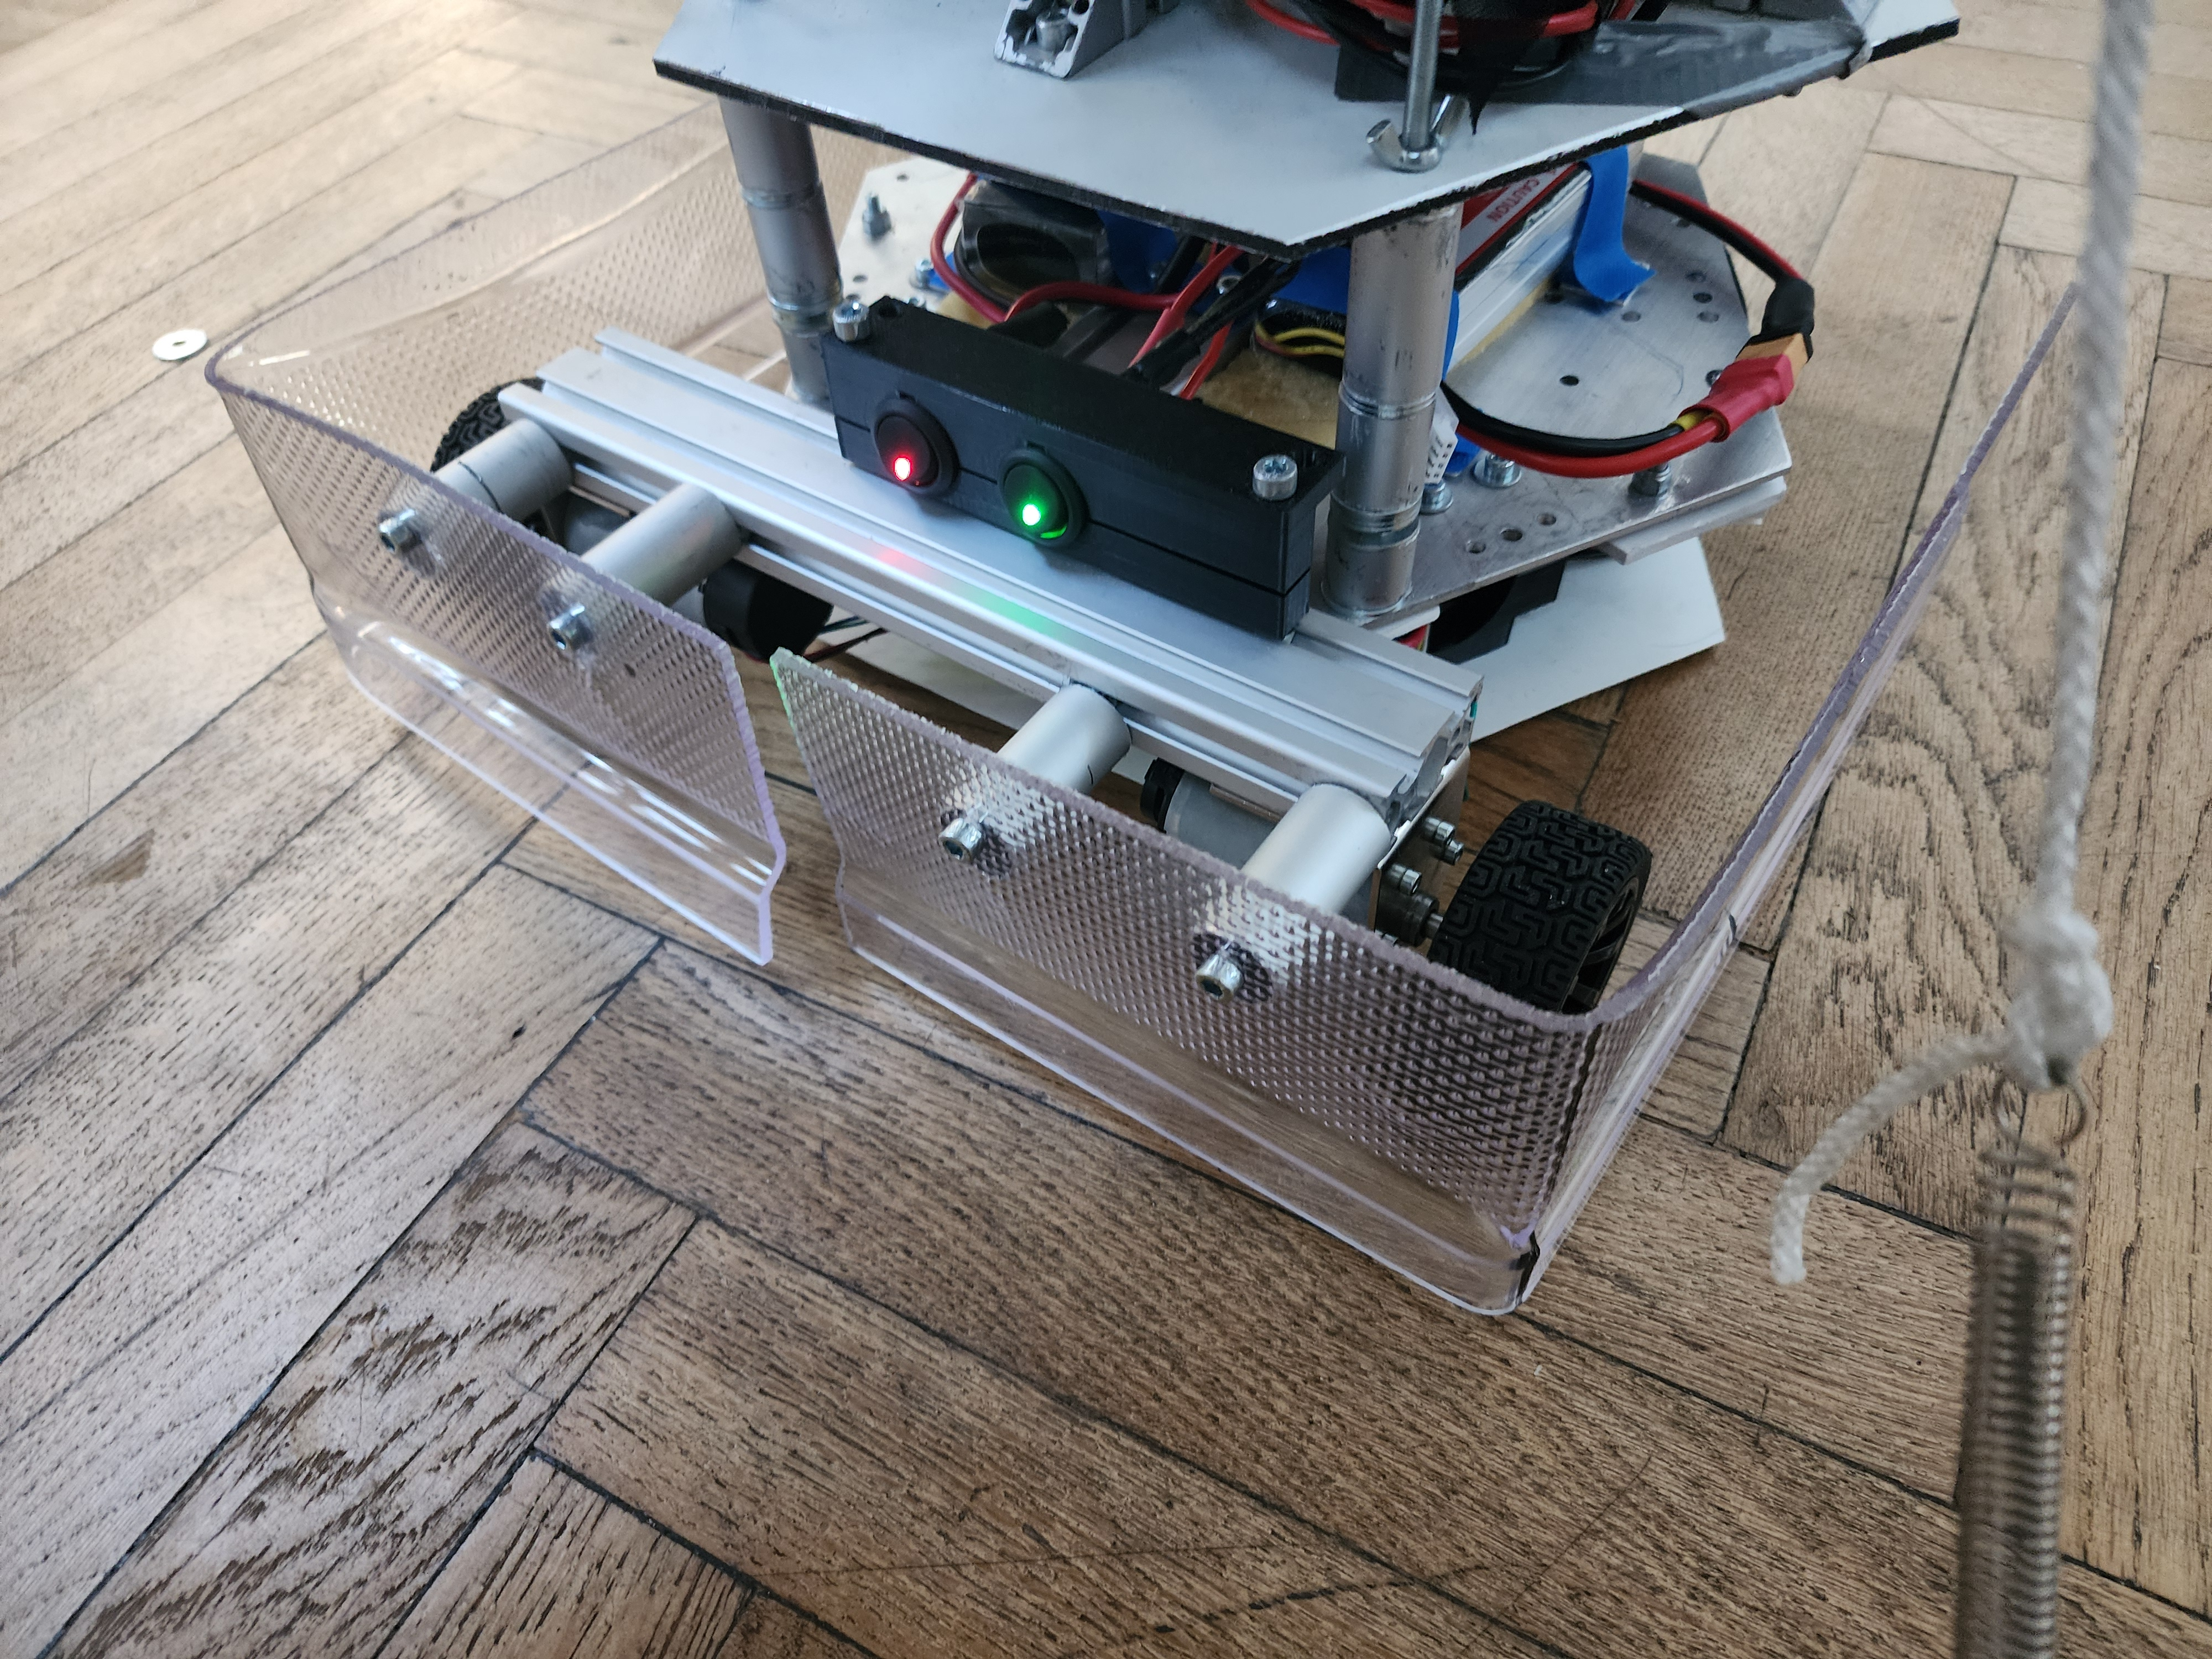
\includegraphics[width=\textwidth]{Images/TinoBumper (4).jpg}
        \caption{Tino Bumper Front View}
        \label{fig:tino_bumper_front}
    \end{minipage}
    \hfill
    \begin{minipage}{0.45\textwidth}
        \centering
        \includegraphics[width=\textwidth]{Images/TinoBumper (5).jpg}
        \caption{Tino Bumper Top View}
        \label{fig:tino_bumper_top}
    \end{minipage}
\end{figure}

\subsection{Control System Adaptation for Differential Drive}

\begin{figure}[H]
    \centering
    \includegraphics[width=0.8\textwidth]{Images/TinoOnNewBase.jpg}
    \caption{Tino on New Base}
    \label{fig:tino_on_new_base}
\end{figure}

The control system required comprehensive modification to support differential drive kinematics while maintaining compatibility with existing command interfaces.

\subsubsection{Custom PID Controller Implementation}

The PID controller development specifically targets differential drive characteristics, replacing the VirHas library dependency with custom control algorithms optimized for Tino's platform. The implementation utilizes classical PID control with Kp=7.3, Ki=5.6, and Kd=0.2 parameters tuned specifically for the MDD10A motor drivers and Tino's mechanical characteristics.

Motor speed calculation employs encoder feedback with 1920 pulses per revolution (PPR) encoders to determine actual wheel velocities in rad/s. The \texttt{getMotorSpeed()} function calculates instantaneous speed based on encoder position changes over time intervals, enabling closed-loop speed control for precise movement execution.

The \texttt{updatePid()} function implements the complete PID algorithm with integral term reset on setpoint changes to prevent windup, derivative calculation for damping, and output limiting to ±255 PWM range. This ensures stable motor control without oscillation while maintaining responsive movement characteristics.

Atomic movement control integrates with the PID system through the \texttt{updateBaseMovementByTime()} function that manages four distinct movement states: resting (0), little push (1), timing preparation (2), and coordinated forward movement (3). Each state implements specific timing profiles and movement patterns that support synchronized leg-base coordination for VR integration.

The movement state machine ensures atomic operation completion where each movement phase must finish before accepting new commands, preventing interrupted motions that could compromise synchronized robot behavior. State transitions include proper timing validation and pending command management for seamless VR user interaction.

\section{Power Supply System Redesign for Orin Nano}

The power system redesign addresses the comprehensive requirements of the NVIDIA Orin Nano platform and associated high-performance components, necessitating complete architecture overhaul from the legacy Raspberry Pi power distribution system.

\subsection{Power Requirements Analysis and System Specifications}

The NVIDIA Orin Nano platform introduces significantly different power requirements compared to the original Raspberry Pi system, requiring comprehensive power architecture redesign to support enhanced computational capabilities.

\subsubsection{Orin Nano Power Consumption Characteristics}

The Orin Nano requires 19V DC input with power consumption characteristics that reach up to 2A during maximum computational load scenarios including simultaneous SLAM processing, human detection, audio processing, and ROS2 node operation. Typical operational consumption ranges between 1.3A to 1.4A during standard social interaction scenarios.

Power consumption analysis under various operational modes demonstrates peak consumption of 38W during maximum load conditions, with sustained operation typically requiring 25-27W. The power profile exhibits significant variation based on computational load, requiring robust power delivery capable of handling transient peaks without voltage drop.

Computational load correlation shows direct relationship between power consumption and processing intensity, with SLAM operations, TensorRT inference, and audio processing contributing the highest power demands. The variable load characteristics necessitate stable power delivery across the full operational range.

\subsubsection{Auxiliary System Power Requirements}

The Oak-D Pro camera system requires 5V DC input with power consumption up to 5W during high-resolution stereo processing. The camera power can be supplied directly from the Orin Nano USB ports or through dedicated power distribution for enhanced flexibility and reduced main processor loading.

The onboard router system requires 5V DC input for network connectivity and VR communication capabilities. Router power consumption remains relatively constant at approximately 3W during operational periods, providing stable power requirements for system design.

Total system power budget analysis indicates maximum power consumption of approximately 46W under peak operational conditions, with typical sustained operation requiring 33-35W. The power analysis includes safety margins for component aging and environmental variations.

\subsection{DC-DC Converter Implementation and Power Distribution}

The power conversion system utilizes high-efficiency DC-DC converters to transform battery voltage to the multiple voltage levels required by system components.

\subsubsection{Oumefar 12V to 19V Step-Up Converter Selection}

The Oumefar DC-DC step-up converter provides stable 19V output from 12V battery input with efficiency ratings exceeding 85\% across the operational load range. Converter selection prioritized stability, efficiency, and thermal performance under the sustained loading conditions required for social robot operation.

Power delivery stability testing demonstrated consistent voltage regulation within ±2\% across full load range with excellent transient response during computational load variations. Thermal performance analysis shows acceptable operating temperatures during sustained maximum load conditions without additional cooling requirements.

Load regulation characteristics maintain stable 19V output from no-load to maximum current draw, ensuring consistent Orin Nano performance across all operational scenarios. The converter includes overcurrent protection and thermal shutdown features that protect against component failure during fault conditions.

\subsubsection{Secondary Power Rail Implementation}

The 12V to 5V conversion system provides power for auxiliary components including the Oak-D Pro camera and onboard router. The secondary converter selection prioritized efficiency and multiple output capability to support various system components.

Power distribution architecture enables independent power control for auxiliary components, providing flexibility for future system expansion and reduced loading on the primary Orin Nano power rail. The distributed approach improves system reliability by isolating power domains.

Circuit protection includes individual fusing for each power rail and overcurrent protection that prevents system damage during component failure scenarios. The protection scheme enables continued operation of unaffected systems during partial power system failures.

\subsection{Battery System Optimization and Consolidation}

The battery system redesign consolidates multiple power sources while providing enhanced capacity and reliability for extended operational periods.

\subsubsection{Battery Specification and Performance Analysis}

The primary battery system utilizes 5200mAh 80C 11.1V 57.72Wh LiPo batteries that provide the power density and discharge capabilities required for robotic applications. Battery specification analysis demonstrates adequate capacity for 2-3 hours of typical operation with conservative discharge management.

Maximum load operational time calculations indicate approximately 1.37 hours of operation under peak power conditions, though realistic operational scenarios typically achieve 2+ hours due to variable computational loading.

Discharge characteristics analysis demonstrates stable voltage delivery throughout the operational range with minimal voltage drop during high current transients. The high discharge rate capability (80C) ensures stable power delivery during computational peaks without voltage sag.

\subsubsection{Power System Consolidation Strategy}

The system consolidation reduces complexity from four separate battery systems to three integrated power sources, eliminating the dedicated router power bank and USB power bank previously required for Raspberry Pi operation. Consolidation simplifies system startup procedures and reduces component count.

Battery management strategy includes individual monitoring and charging protocols for each power source while maintaining operational independence. The consolidated approach reduces overall system weight while providing enhanced operational capability through optimized power distribution.

Operational startup sequence simplifies through power system consolidation, reducing from multiple power-on procedures to streamlined system activation. The simplified approach reduces operator complexity and potential startup errors during experimental scenarios.

\subsection{Cable Harness Redesign and Integration}

The cable harness redesign eliminates legacy connections while implementing proper power distribution for the enhanced system architecture.

\subsubsection{Legacy Connection Removal and Modernization}

The cable harness modification removes obsolete USB-A and USB-C connections that were utilized for Raspberry Pi power delivery, replacing them with proper 12V distribution and 19V DC jack connectivity optimized for Orin Nano requirements. Connector selection prioritizes reliability and ease of maintenance.

Cable routing optimization reduces electromagnetic interference and mechanical stress while providing secure connections throughout the system. Harness design includes service loops and strain relief that accommodate system maintenance without cable damage.

Connector standardization utilizes consistent connector types throughout the system to simplify maintenance and reduce spare parts requirements. Standardization also reduces connection errors during system assembly and troubleshooting procedures.

\subsubsection{Power Distribution Architecture}

The 12V input distribution system provides primary power for both the step-up converter and the secondary 5V converter, enabling efficient power utilization from the primary battery source. Distribution includes proper circuit protection and monitoring capabilities.

The 19V DC jack implementation provides secure power connection to the Orin Nano with proper mechanical support and electrical contact reliability. Jack selection includes locking mechanisms that prevent accidental disconnection during operation.

Future expansion capabilities include additional power distribution points for system upgrades and experimental equipment integration. The modular power architecture supports system enhancement without complete harness redesign.

\section{Stewart Platform Head Mechanism Improvements}

The Stewart platform head mechanism underwent iterative design improvements to address systematic reliability issues and enhance performance under the operational loads encountered during social robot interaction scenarios.

\subsection{Original System Analysis and Failure Modes}

The original Stewart platform implementation exhibited multiple failure modes that compromised head movement precision and system reliability during extended operational periods.

\subsubsection{Servo Axis Misalignment Problems}

The original design suffered from servo axis misalignment that created excessive stress concentrations on servo motor internals during head movement operations. Force analysis revealed that head loads were transmitted directly through servo shafts rather than through the structural framework, creating potential failure-prone stress concentrations.

The misalignment created moment arms that amplified forces applied to servo components, requiring design revision to prevent potential servo damage. The servo axis alignment improvement was implemented as a preventive measure to ensure reliable long-term operation.

Mechanical analysis demonstrated that proper force transmission should flow through the head structure rather than servo mechanisms, necessitating fundamental design revision to achieve reliable operation under Tino's operational requirements.

\subsubsection{Structural Flexibility and Arm Failures}

The connecting arms exhibited excessive structural flexibility that reduced head positioning precision and contributed to mechanical instability during movement sequences. Flex analysis revealed inadequate stiffness-to-weight ratio in the original arm design, creating unwanted compliance in the kinematic chain.

Repeated arm failures occurred due to inadequate load distribution and material selection that could not withstand the combination of static head weight and dynamic movement forces. Failure analysis identified stress concentration points where 3D printed components experienced crack initiation and propagation.

Material selection limitations in PLA printing created brittleness under repeated loading cycles, with failure modes including layer delamination and stress cracking at critical load transfer points. The original material selection proved inadequate for the sustained loading requirements of social robot head movement.

\subsection{First Design Iteration: Servo Axis Alignment}

The first improvement iteration focused on servo axis alignment to redirect forces through proper load paths while maintaining the existing bearing-based connection system.

\begin{figure}[H]
    \centering
    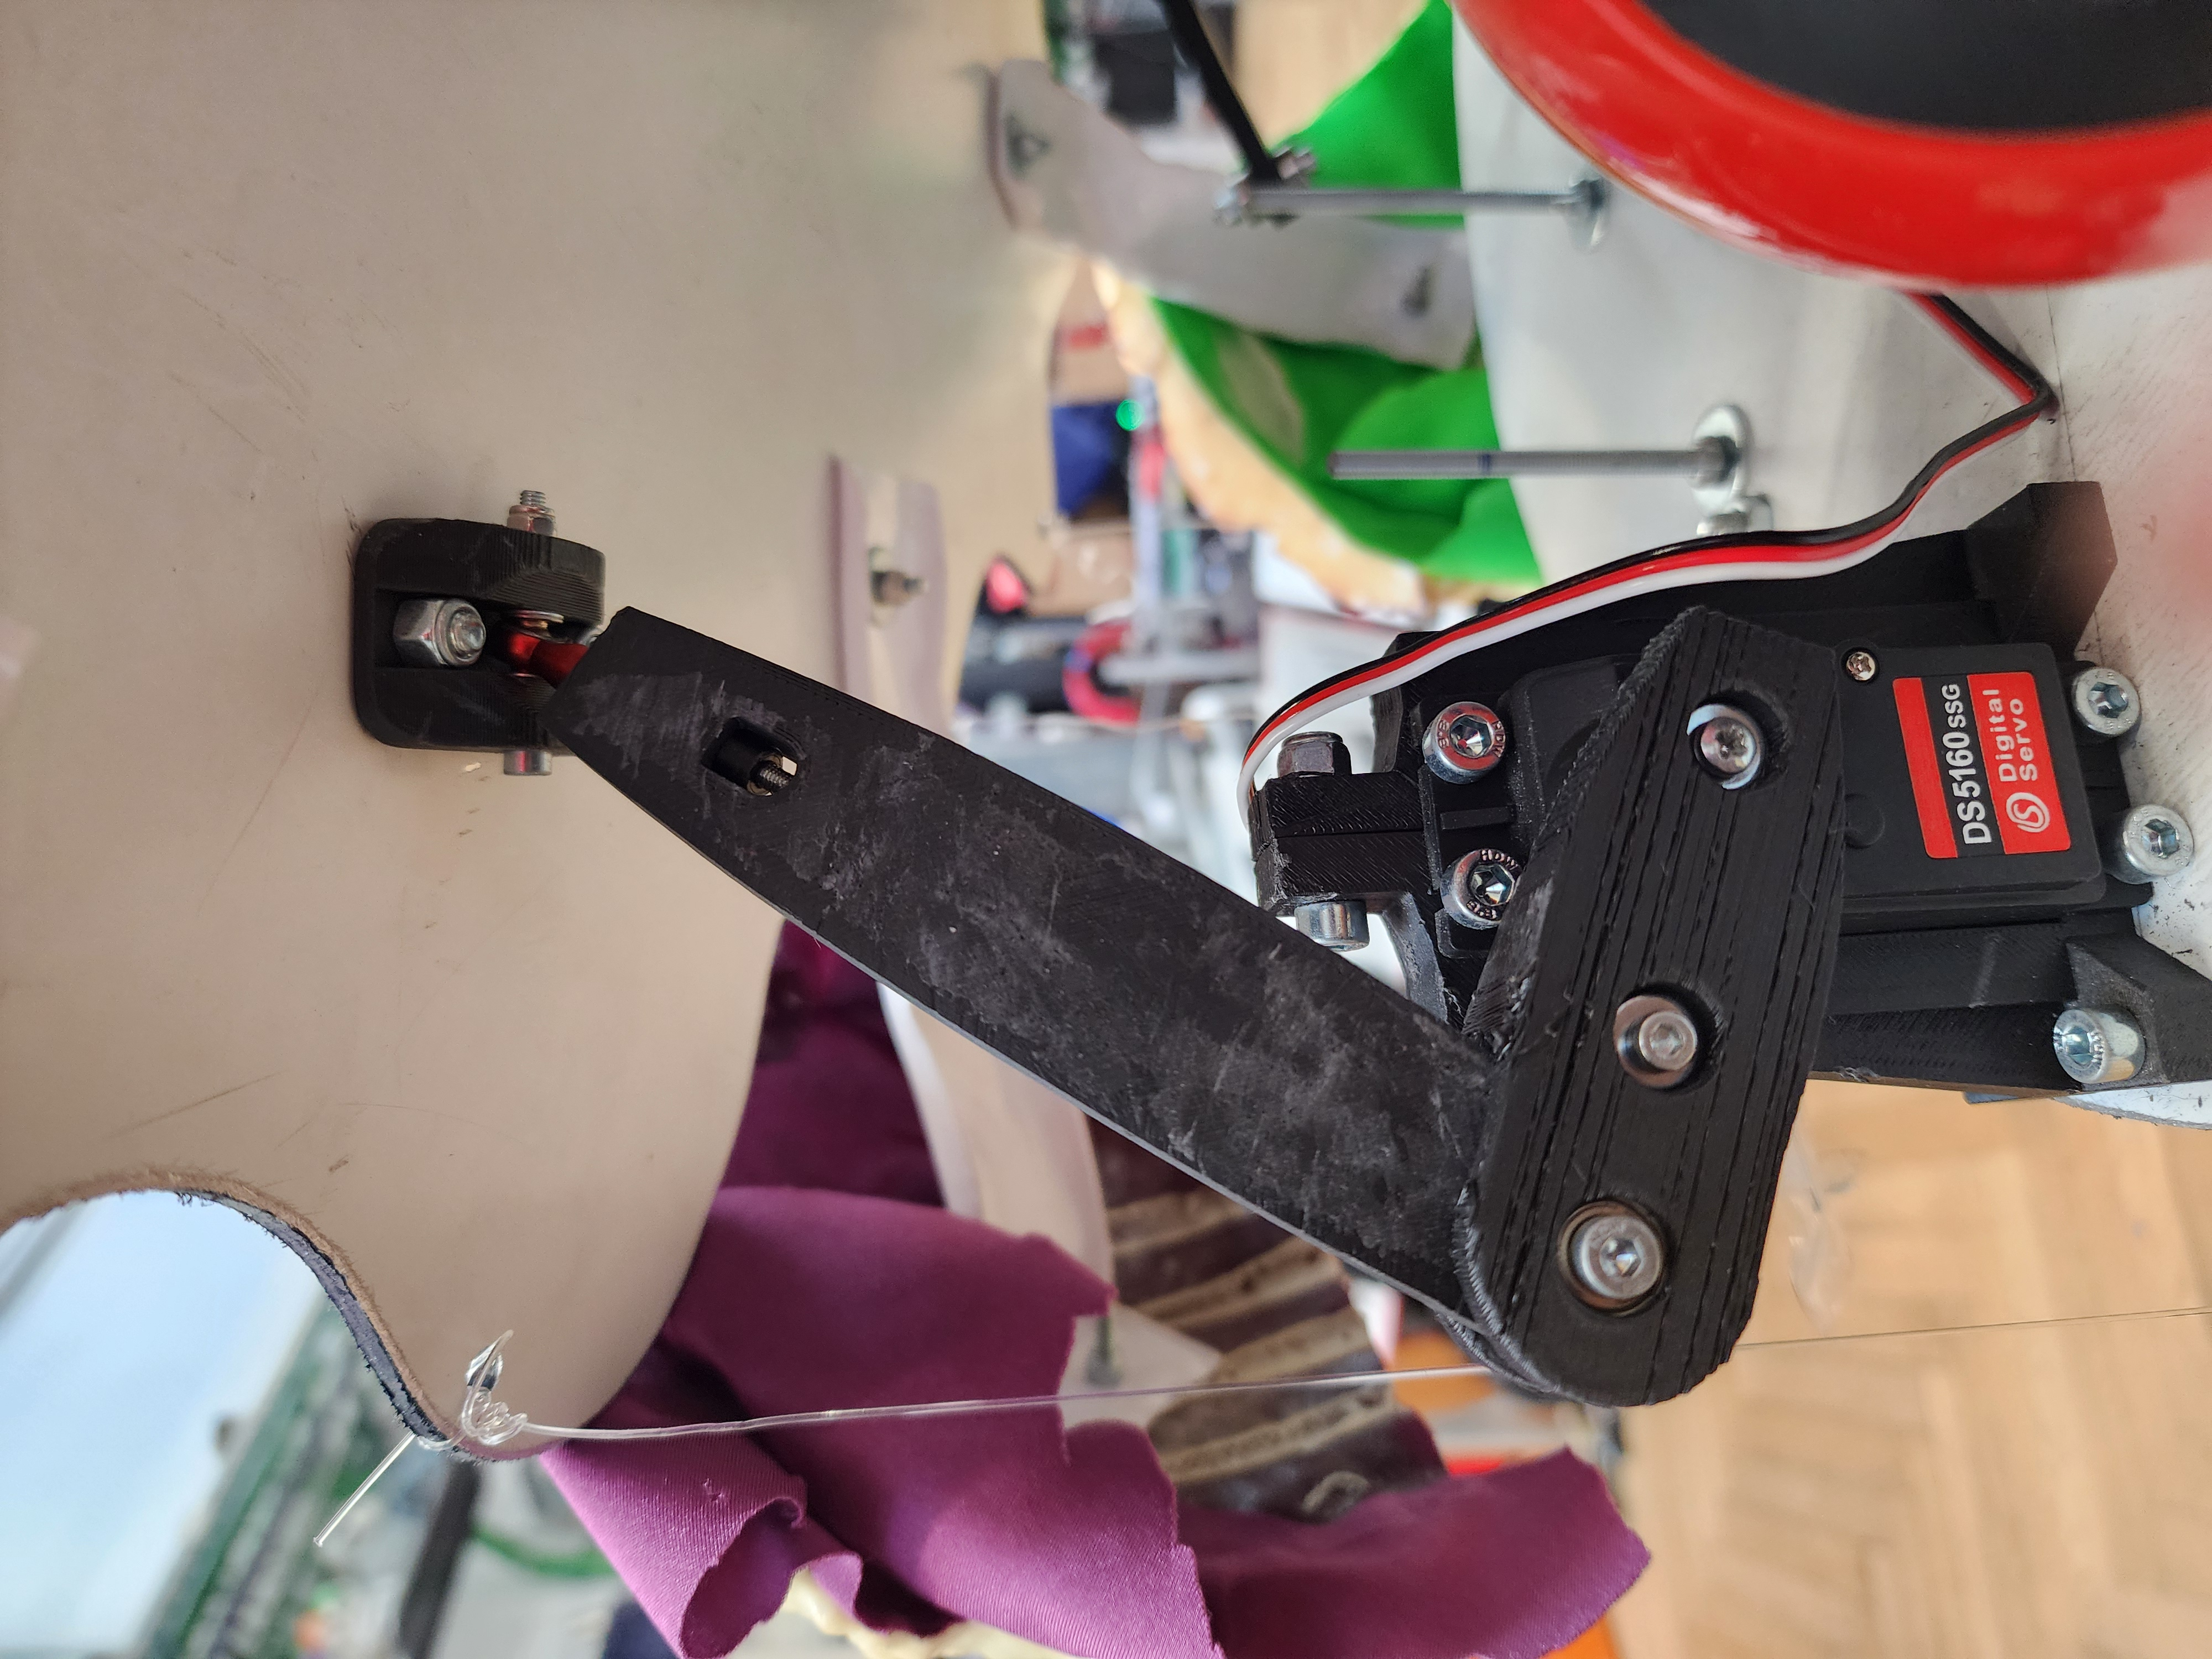
\includegraphics[height=6cm, angle=-90]{Images/HeadArmV2.jpg}
    \caption{Head Arm V1 Design}
    \label{fig:head_arm_v1}
\end{figure}

\subsubsection{Force Path Optimization}

The servo axis alignment improvement redirected head loads through the structural framework rather than servo mechanisms, reducing stress concentrations in servo internal components. Force analysis demonstrated significant reduction in lateral servo loading through proper geometric alignment.

Structural load distribution optimization utilized improved geometry to distribute head weight and movement forces across the Stewart platform structure. Load path analysis verified proper force transmission through structural components rather than servo mechanisms.

Performance evaluation demonstrated reduced servo stress indicators and improved movement precision, though structural flexibility issues remained due to the retained bearing connection system on the servo side of each arm.

\subsubsection{ 3D Printed Component Enhancement}

Enhanced PLA arm geometry provided improved load distribution through optimized cross-sectional design and stress concentration reduction. Geometric optimization utilized finite element analysis principles to identify optimal material distribution within manufacturing constraints.

Print orientation optimization aligned layer structure with primary stress directions to maximize strength characteristics within PLA material limitations. Layer orientation analysis demonstrated significant strength improvement through proper print setup procedures.

Initial performance testing showed improved reliability and reduced failure frequency, though continued structural flexibility limited overall system performance improvement. The partial solution validated the design approach while highlighting remaining system limitations.

\subsection{Persistent Flexibility Issues and Continued Arm Failures}

Despite the servo axis alignment improvements implemented in the first design iteration, the Stewart platform continued to experience significant structural flexibility problems that ultimately led to repeated arm failures during extended operational periods.

\begin{figure}[H]
    \centering
    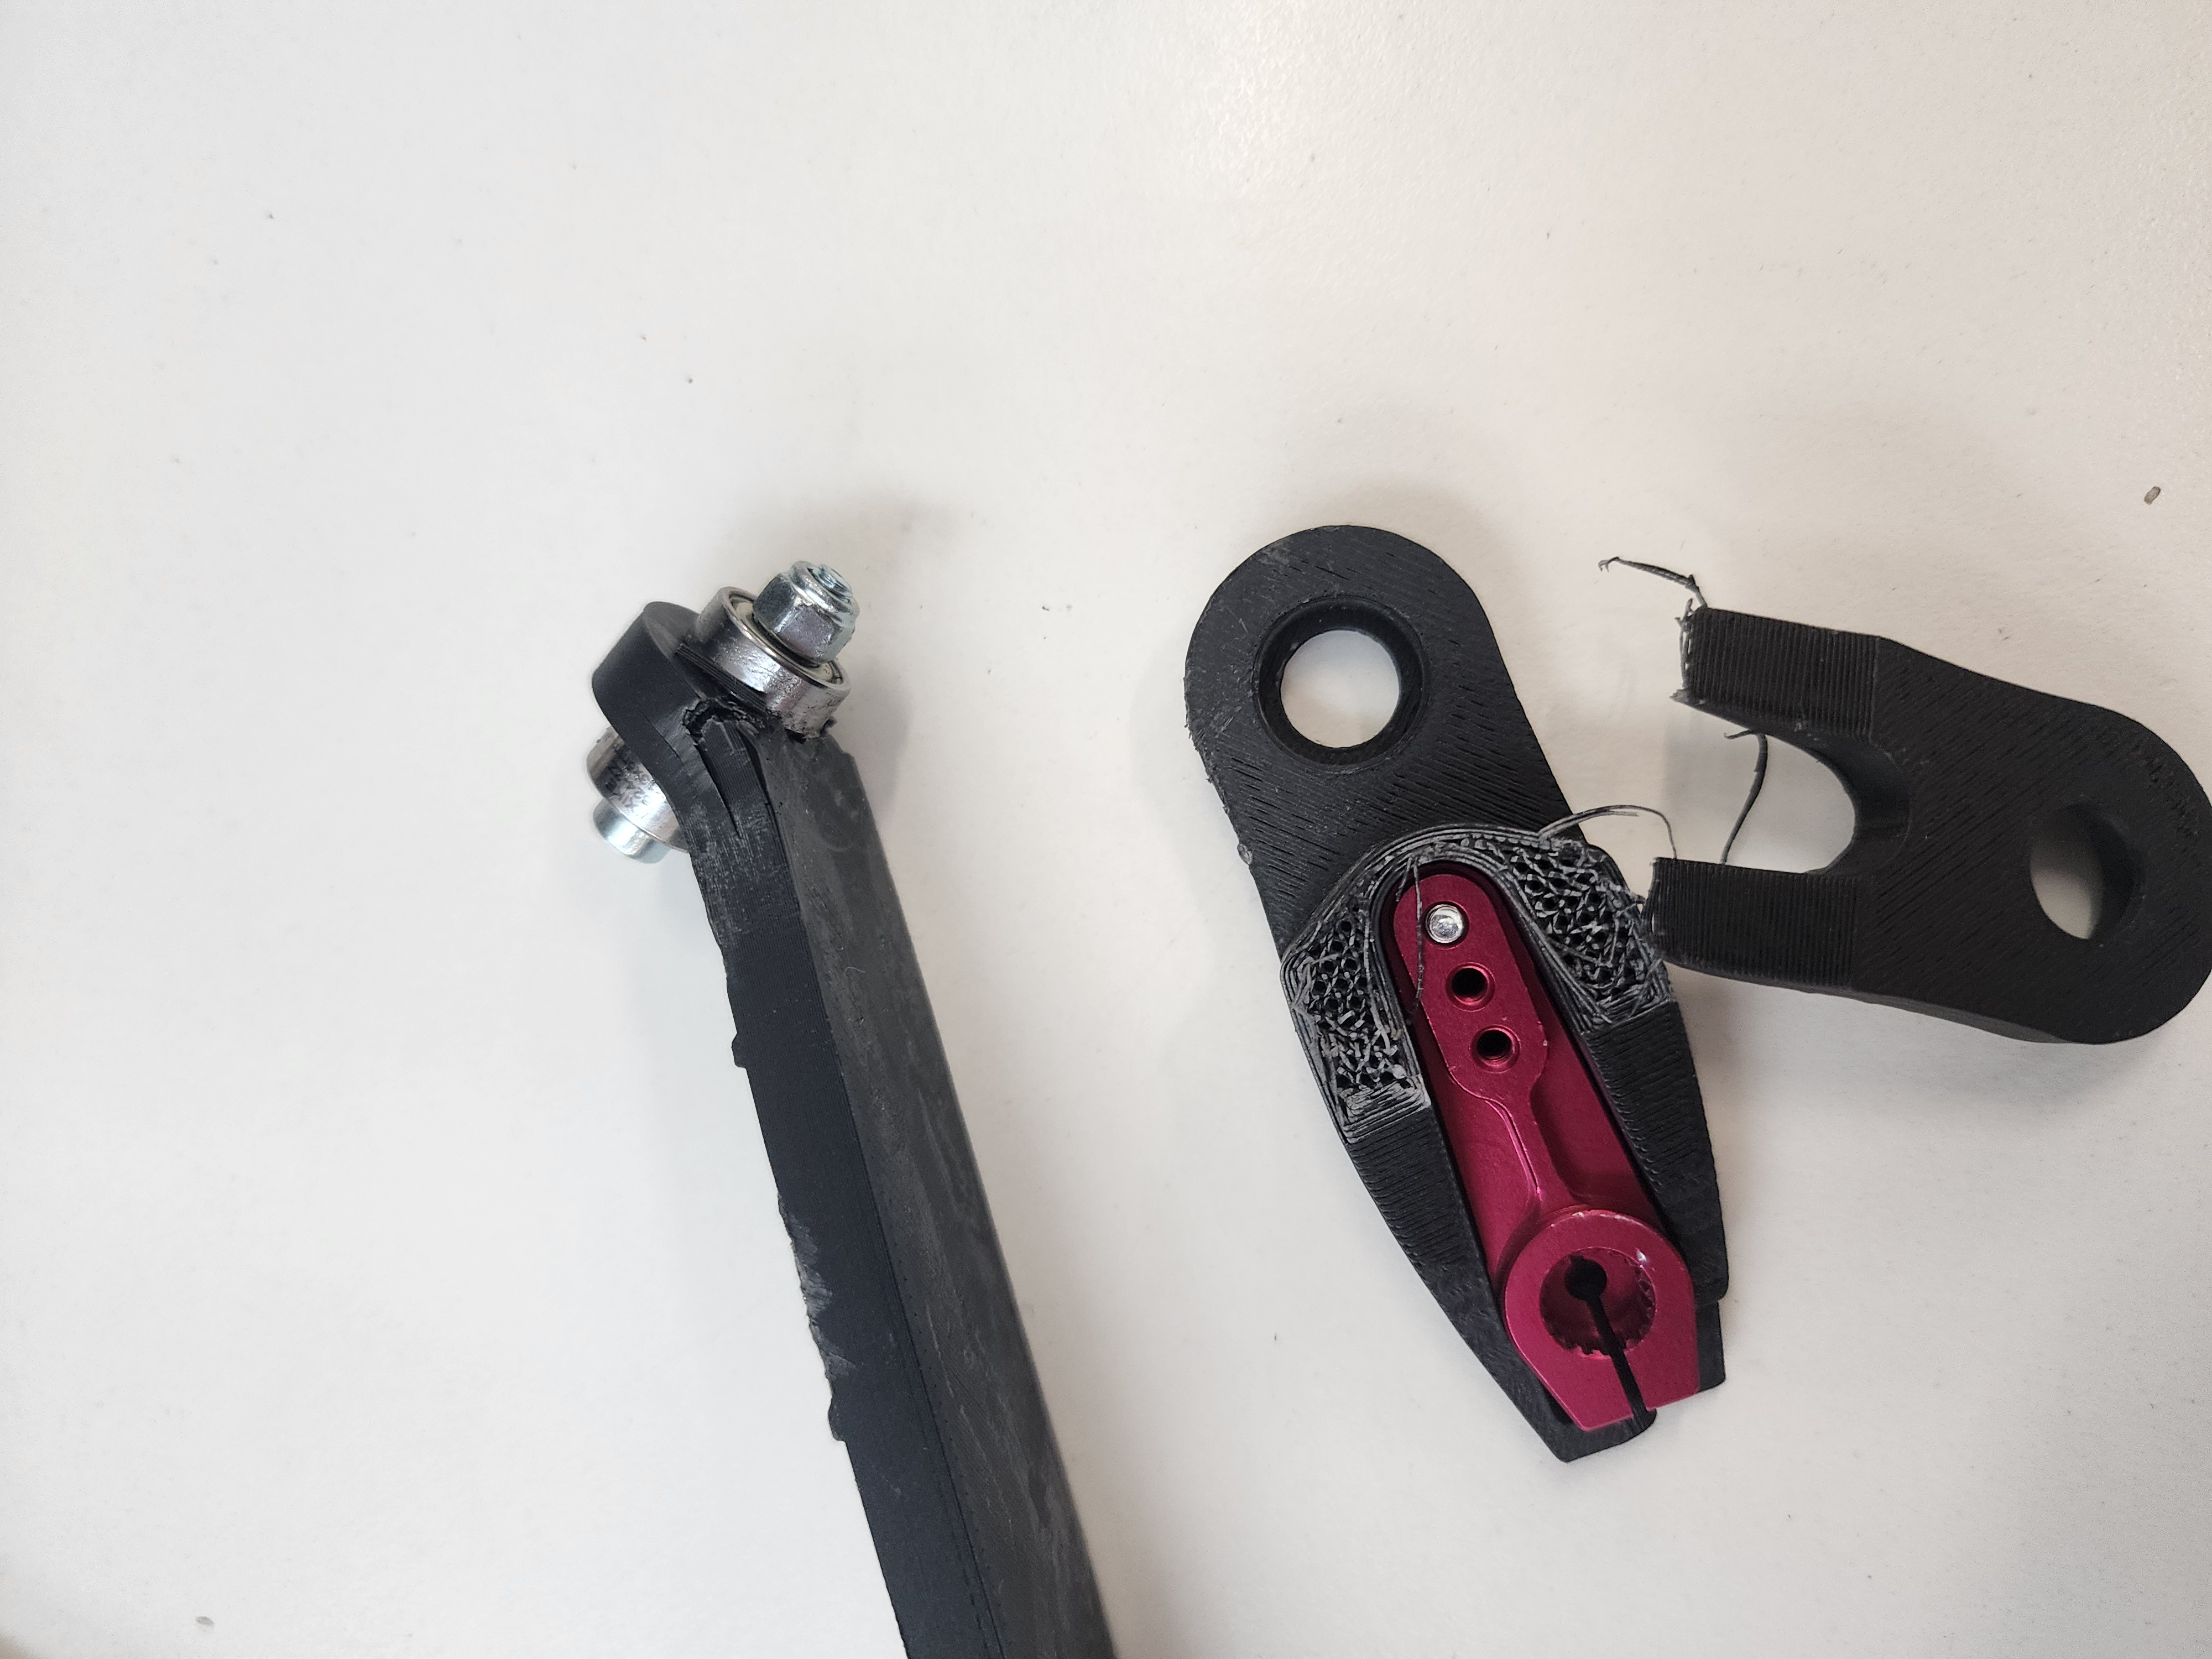
\includegraphics[height=6cm, angle=-90]{Images/HeadArmFailure (2).jpg}
    \caption{Head Arm Failure after Extended Use}
    \label{fig:head_arm_failure}
\end{figure}

\subsubsection{Bearing Connection System Limitations}

The retained bearing connection system on the servo side of each arm introduced excessive compliance that compromised head positioning precision and contributed to continued mechanical instability. The bearing housings, while providing smooth articulation, created weak points in the structural chain that allowed unwanted deflection under operational loads.

Failure analysis revealed that the 3D printed bearing housings could not adequately transfer forces between the improved servo connections and the head platform. The plastic bearing housing geometry, despite geometric optimization, remained insufficient to handle the combination of static head weight and dynamic movement forces encountered during typical social robot operation.

Repeated stress cycling during normal head movement operations caused progressive degradation of the bearing connection points, leading to increased play and eventual structural failure. The bearing system's inherent flexibility, while beneficial for smooth movement, created unacceptable structural compliance that compromised system reliability.

\begin{figure}[htbp]
    \centering
    \begin{minipage}{0.45\textwidth}
        \centering
        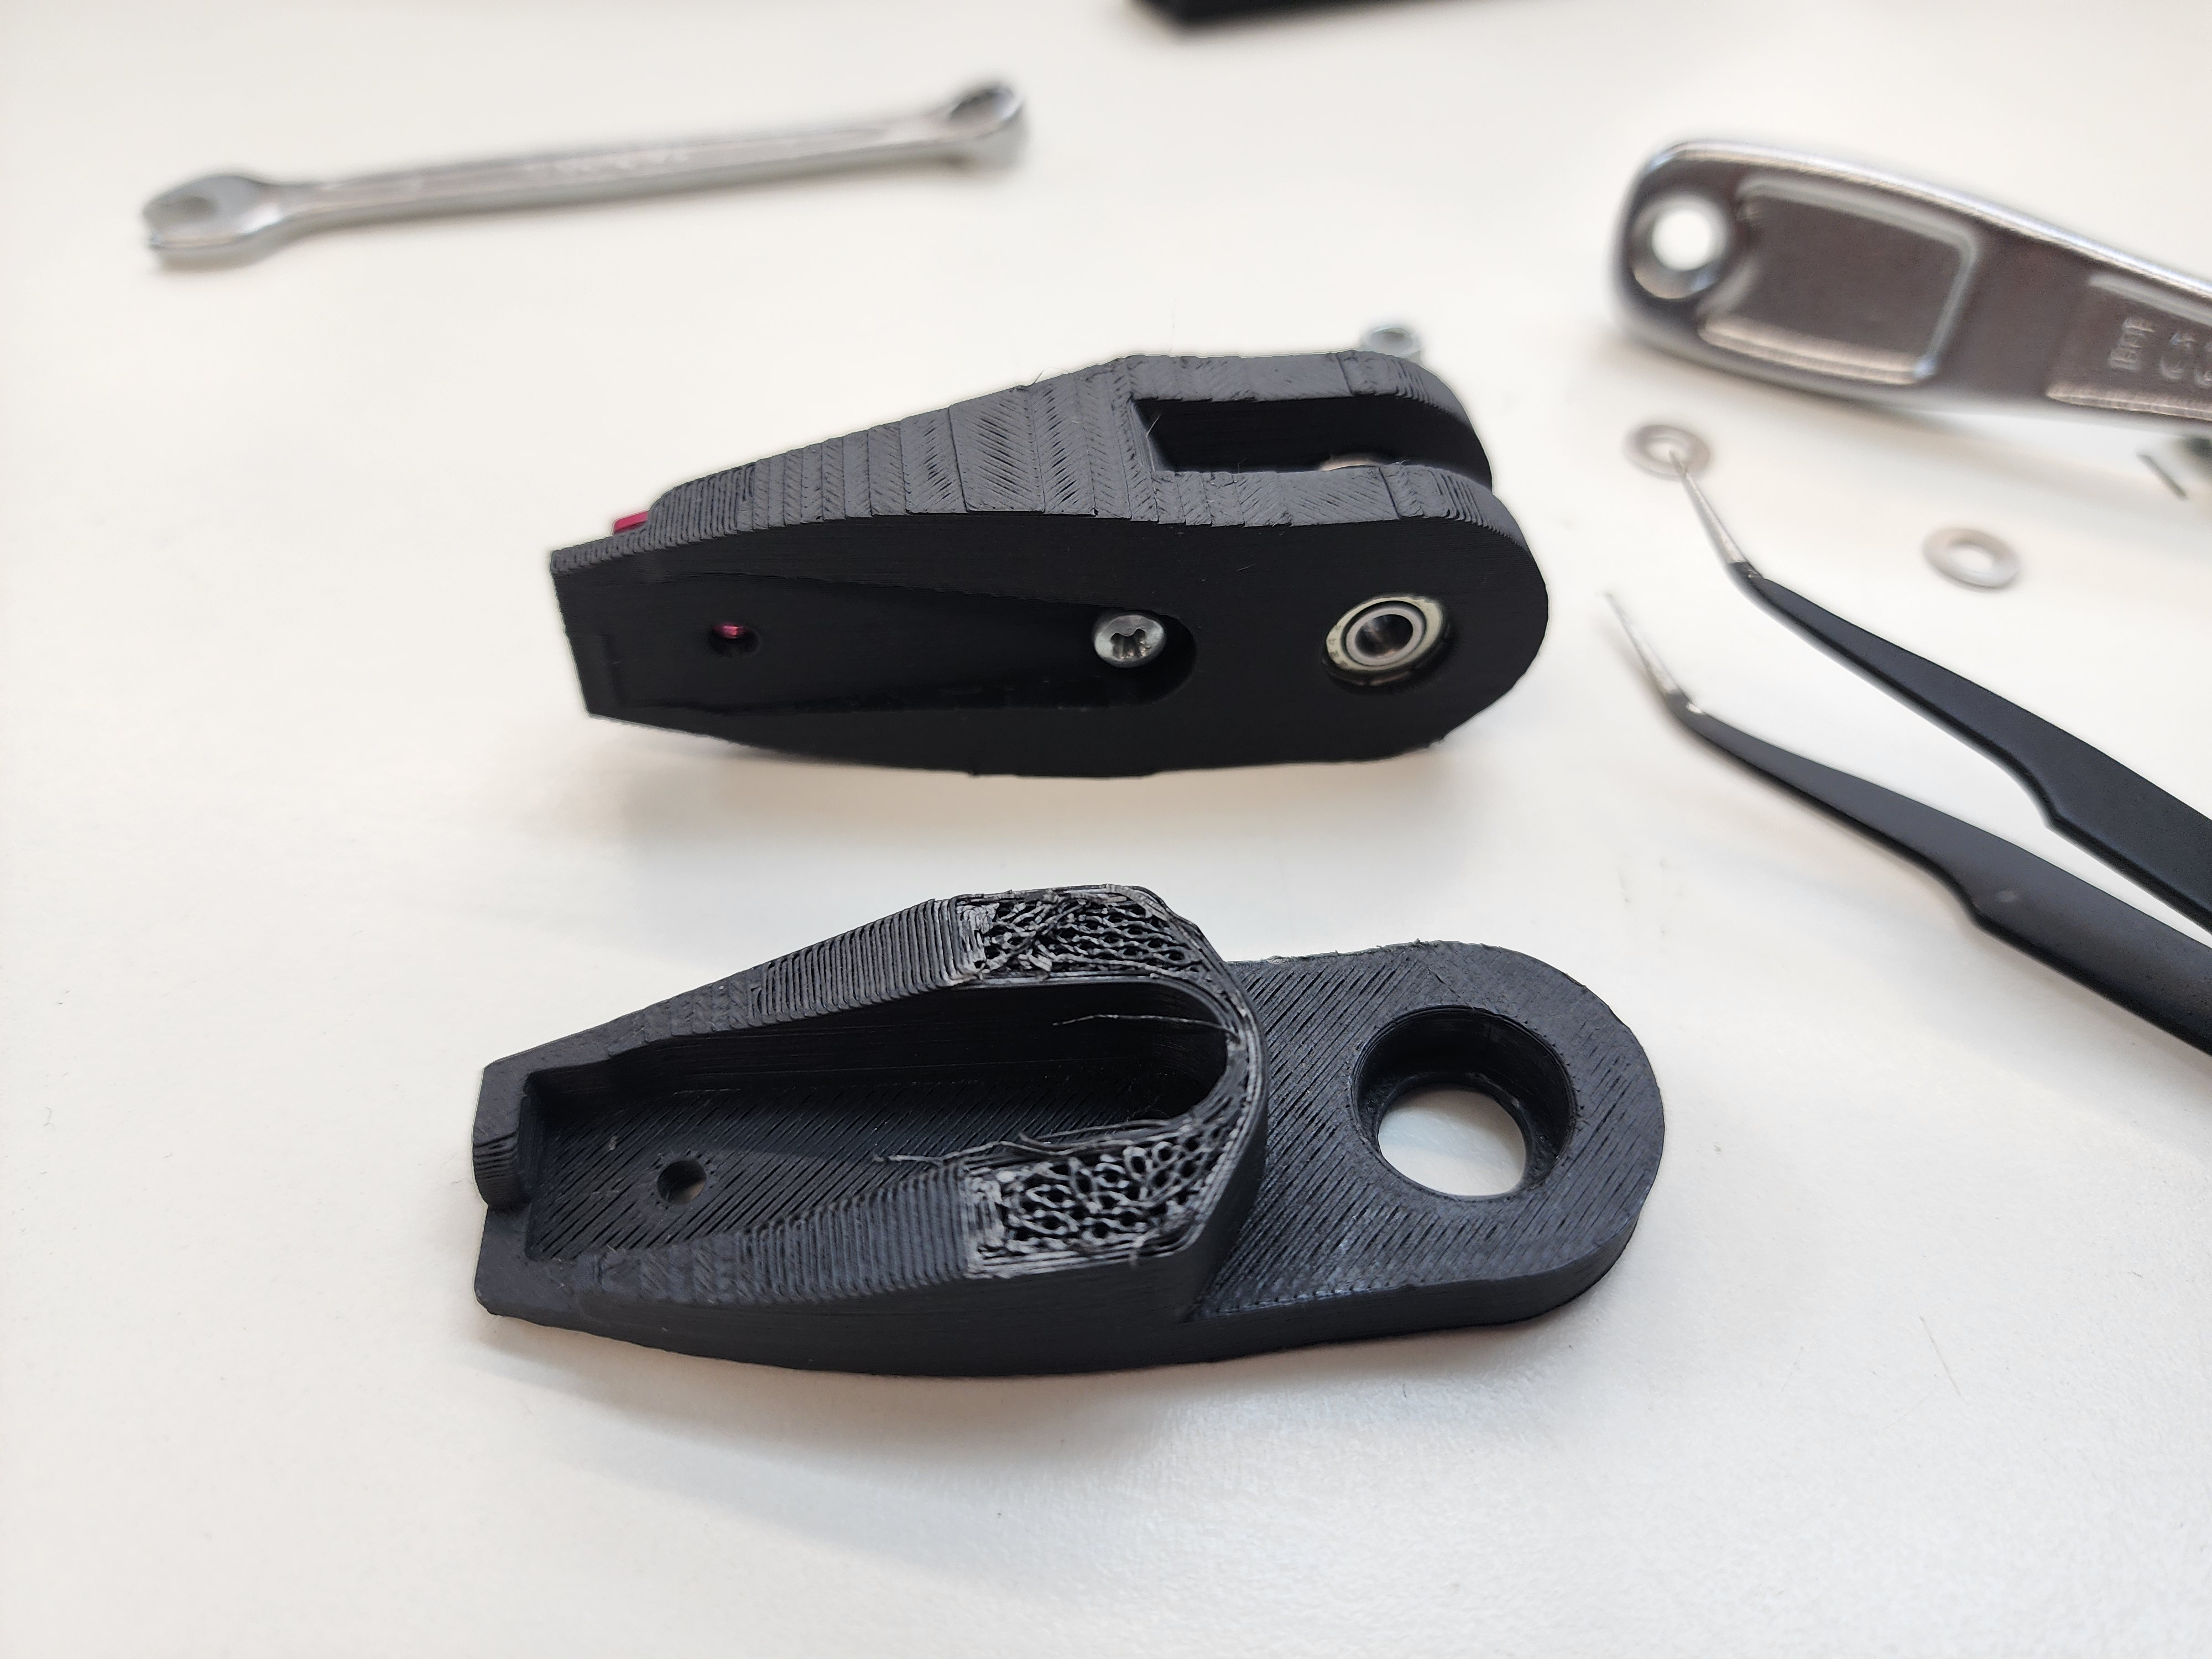
\includegraphics[width=\textwidth]{Images/HeadArmFailure (3).jpg}
        \caption{Servo Side Bearing Connection Failure}
        \label{fig:servo_bearing_failure}
    \end{minipage}
    \hfill
    \begin{minipage}{0.45\textwidth}
        \centering
        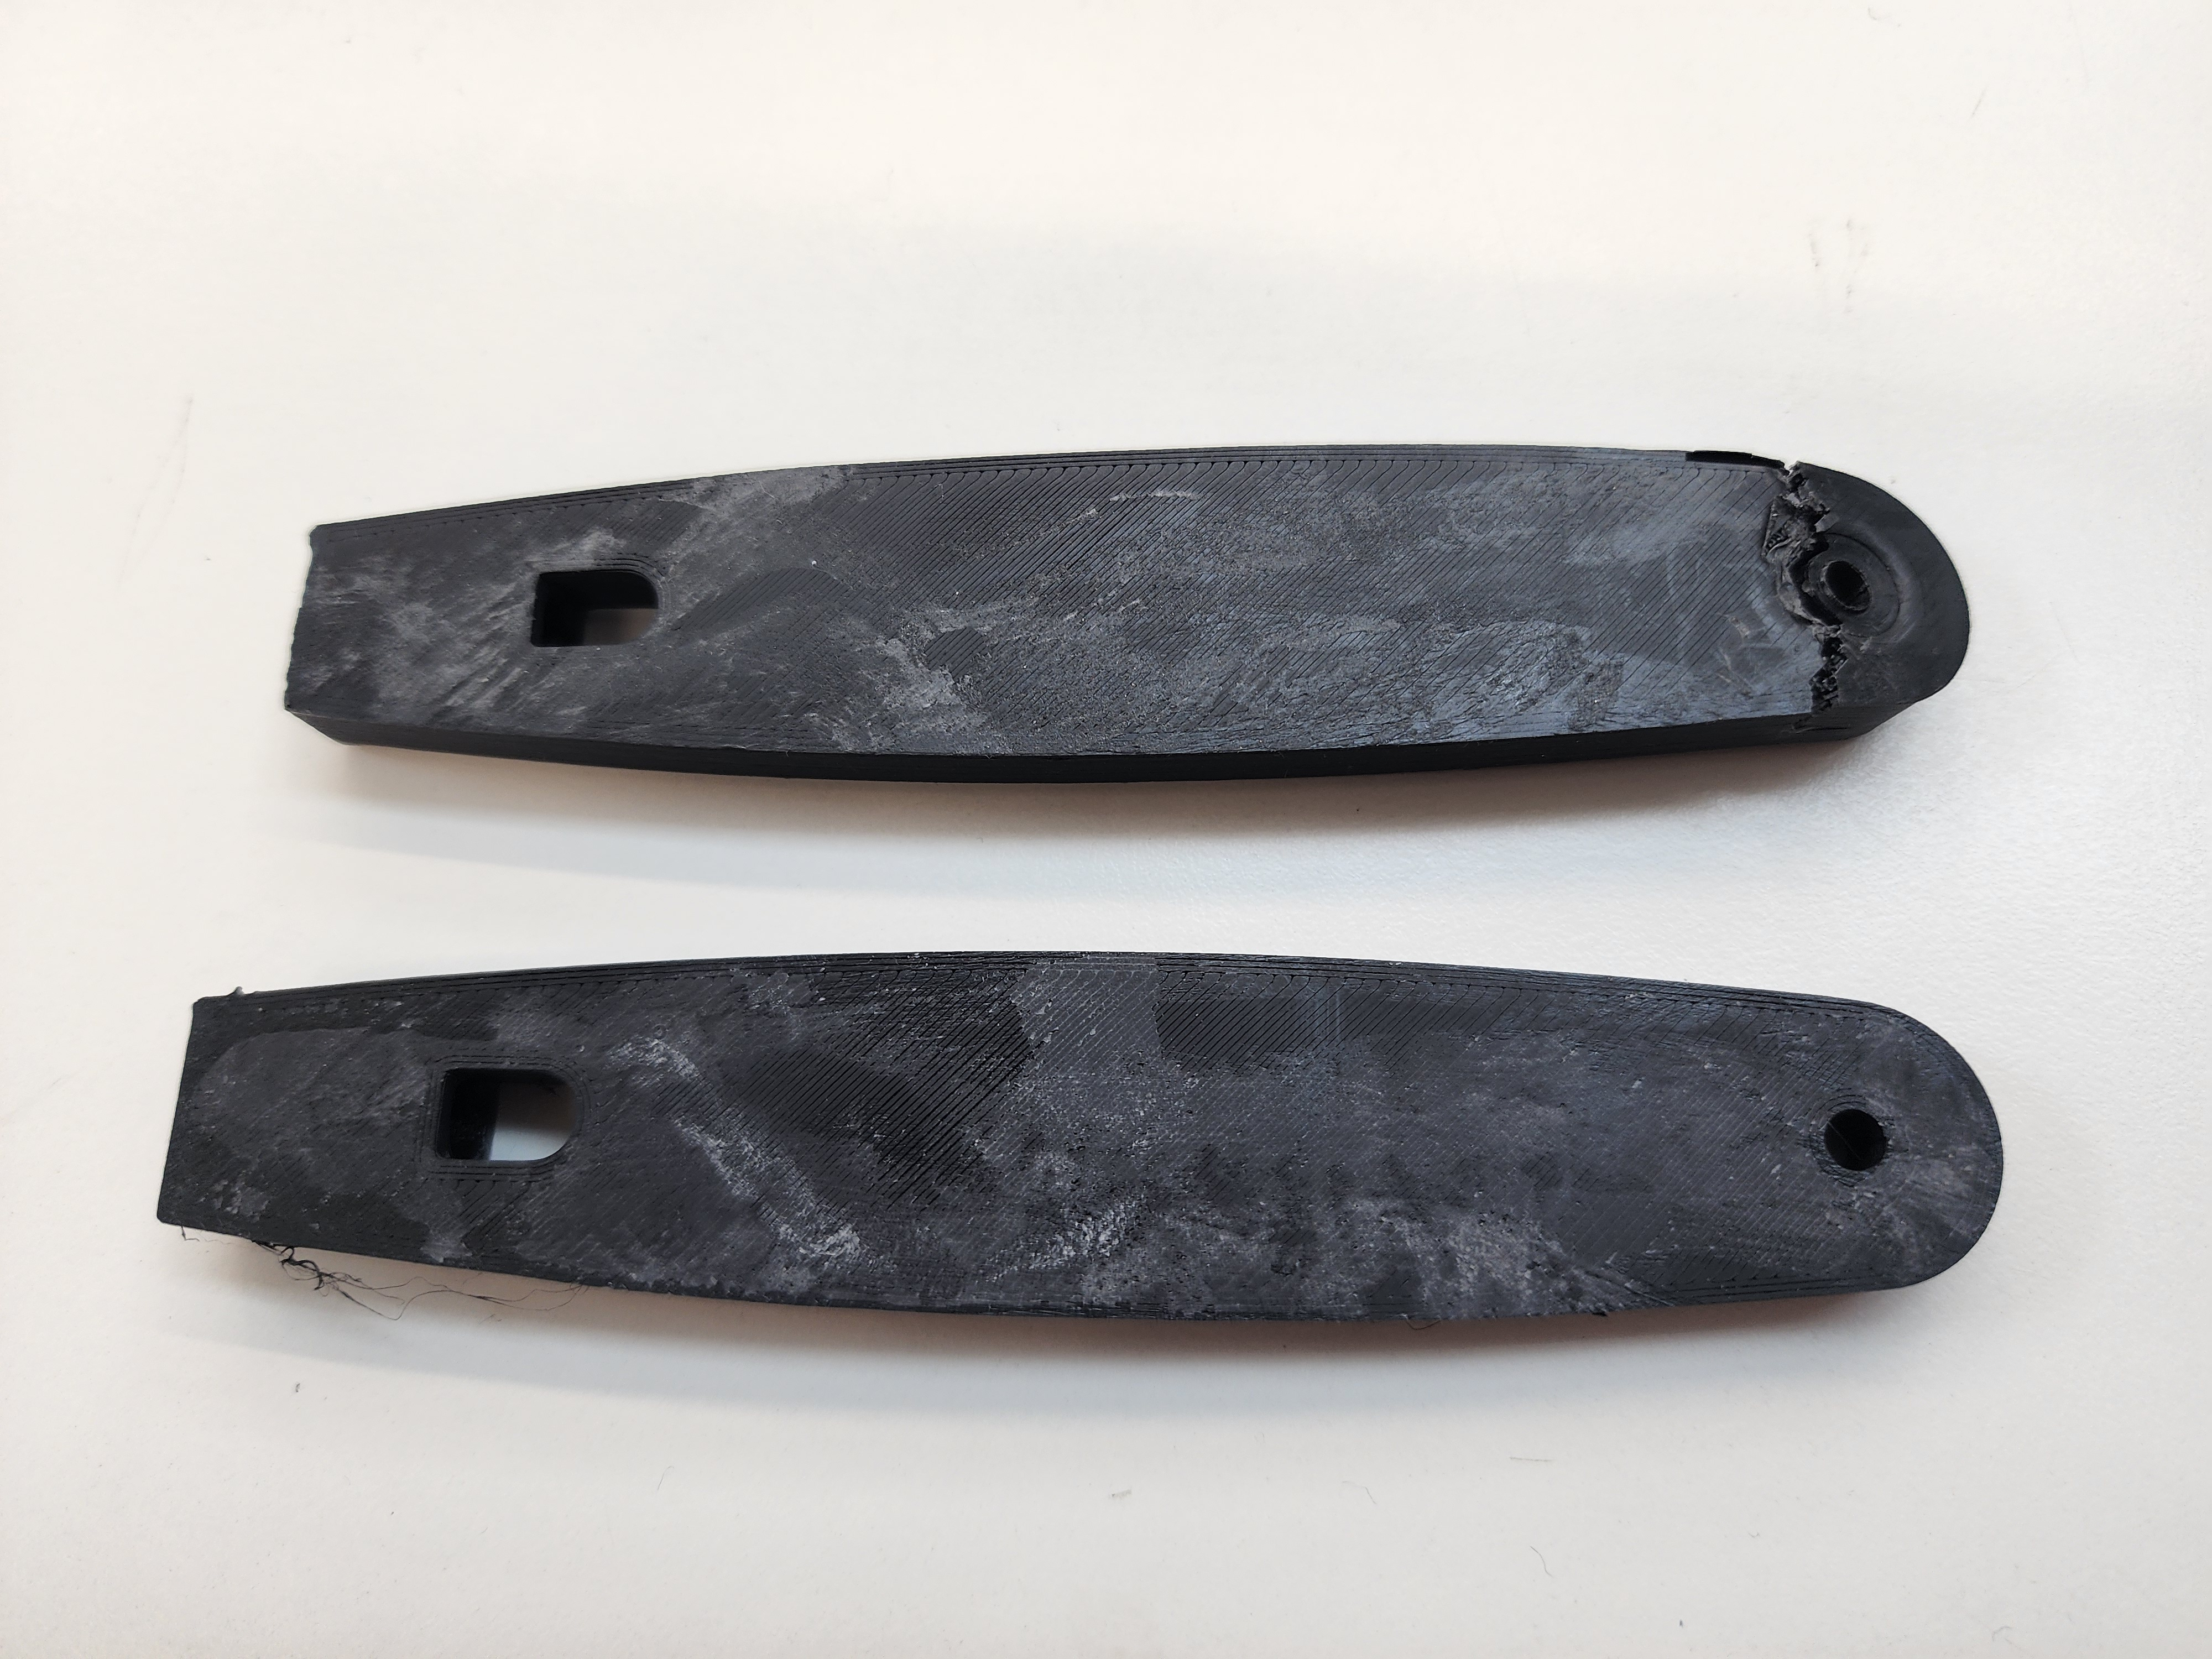
\includegraphics[width=\textwidth]{Images/HeadArmFailure.jpg}
        \caption{Head Arm Failure after Extended Use}
        \label{fig:head_arm_failure}
    \end{minipage}
\end{figure}

\subsubsection{Material and Design Constraint Analysis}

The fundamental limitation resided in the conflict between the need for smooth articulation and structural rigidity within the constraints of 3D printed PLA construction. PLA material properties, while adequate for static structural components, proved insufficient for dynamic load-bearing connections subjected to repeated stress cycles.

Print resolution limitations prevented the creation of bearing surfaces with sufficient precision and durability for sustained operation under Tino's operational loads. Layer adhesion characteristics in PLA created inherent weak points at stress concentration areas around bearing connection points.

The design iteration validated the servo alignment approach while conclusively demonstrating that bearing-based connections could not provide the structural integrity required for reliable long-term operation. These findings necessitated a fundamental redesign approach that would eliminate the problematic bearing connections entirely.

\subsection{Final Design Implementation: Rod End Integration}

The final design iteration addressed remaining flexibility issues through the adoption of rod end (heim joint) connections on both ends of each Stewart platform arm.

\begin{figure}[H]
    \centering
    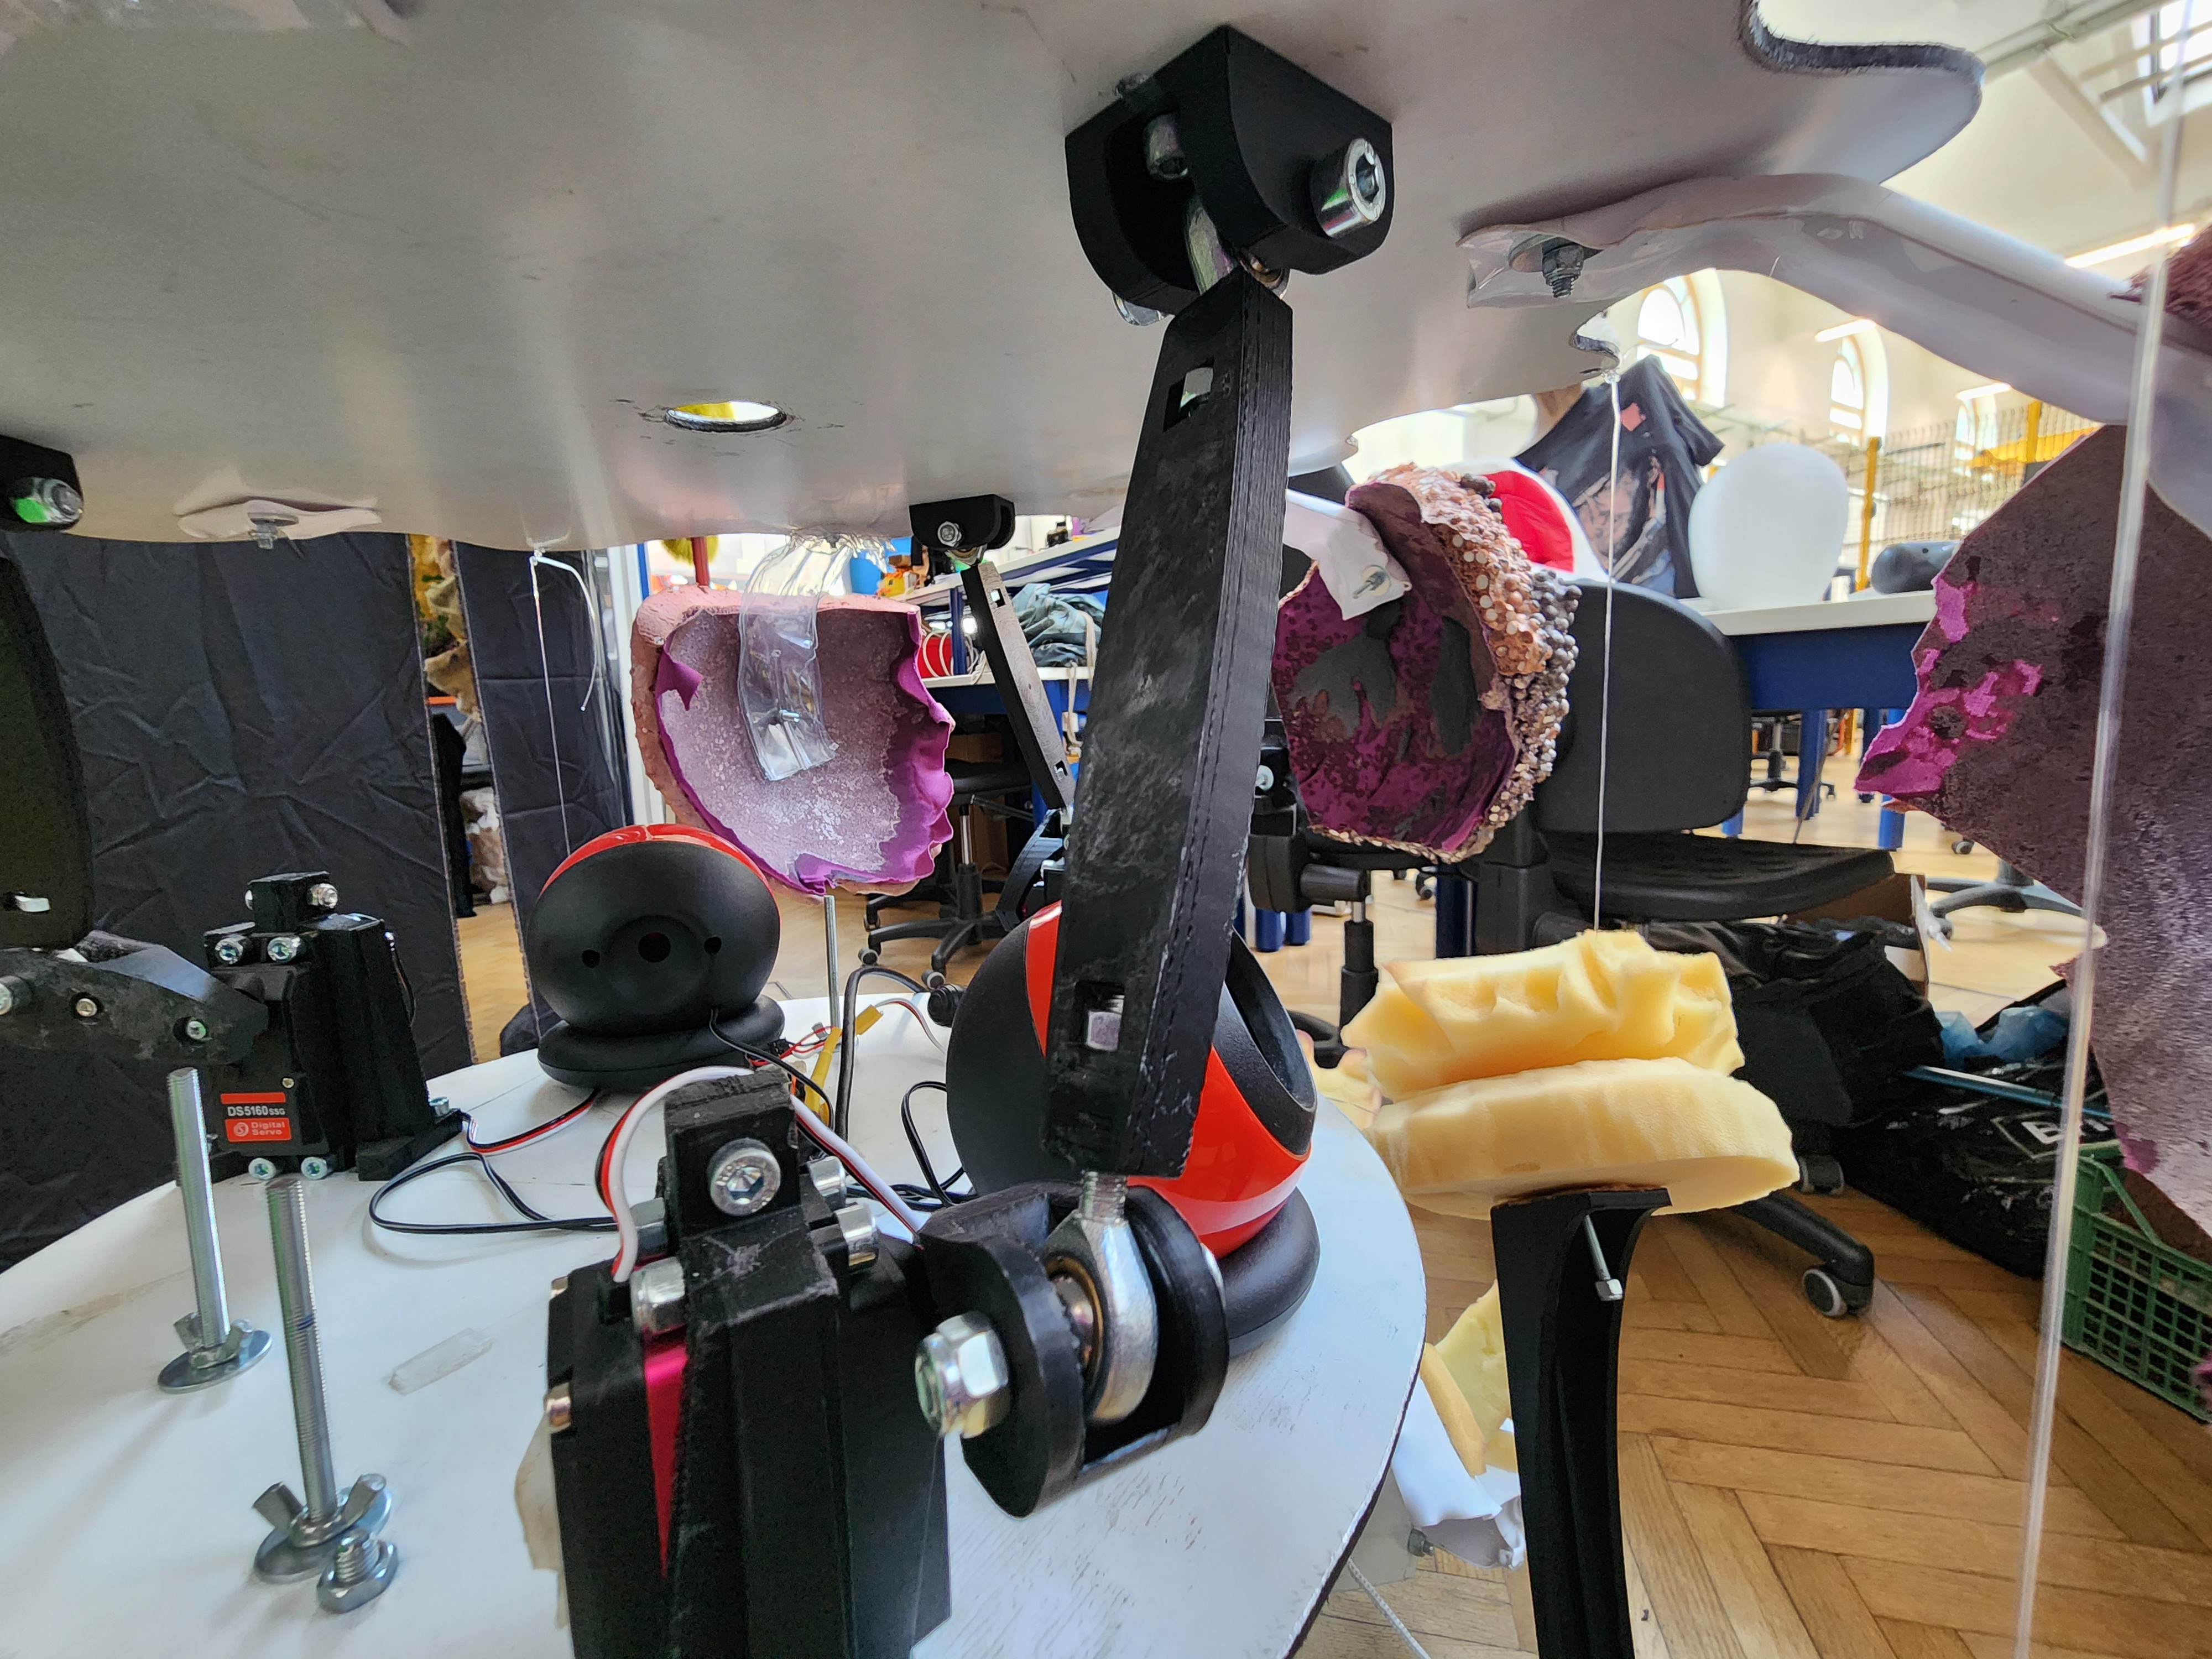
\includegraphics[height=6cm]{Images/NewHeadDoubleJoint (4).jpg}
    \caption{Head Arm V2 Design with Rod Ends}
    \label{fig:head_arm_v2}
\end{figure}

\subsubsection{Rod End Selection and Implementation}

Research into Stewart platform best practices identified rod end connections as the standard solution for eliminating binding while allowing proper articulation throughout the movement range. Rod end selection prioritized load capacity, articulation range, and integration with existing servo and head mounting points.

The rod end implementation utilizes metal heim joints that provide superior strength and durability compared to the original bearing system that used metal bearings encased within 3D printed components. Metal construction eliminates the brittleness and wear issues encountered with the printed bearing housings.

Joint articulation characteristics enable free rotation in all necessary axes while providing positive mechanical connection between arm segments. The rod end design eliminates binding forces that contributed to servo stress and movement precision issues.

\subsubsection{Mechanical Trade-offs and Performance Characteristics}

The rod end implementation introduces acceptable head wobble during stationary periods due to the free articulation provided by the heim joints. Analysis indicates this wobble may actually enhance Tino's expressive capabilities by providing natural movement characteristics.

\begin{figure}[H]
    \centering
    \begin{minipage}{0.45\textwidth}
        \centering
        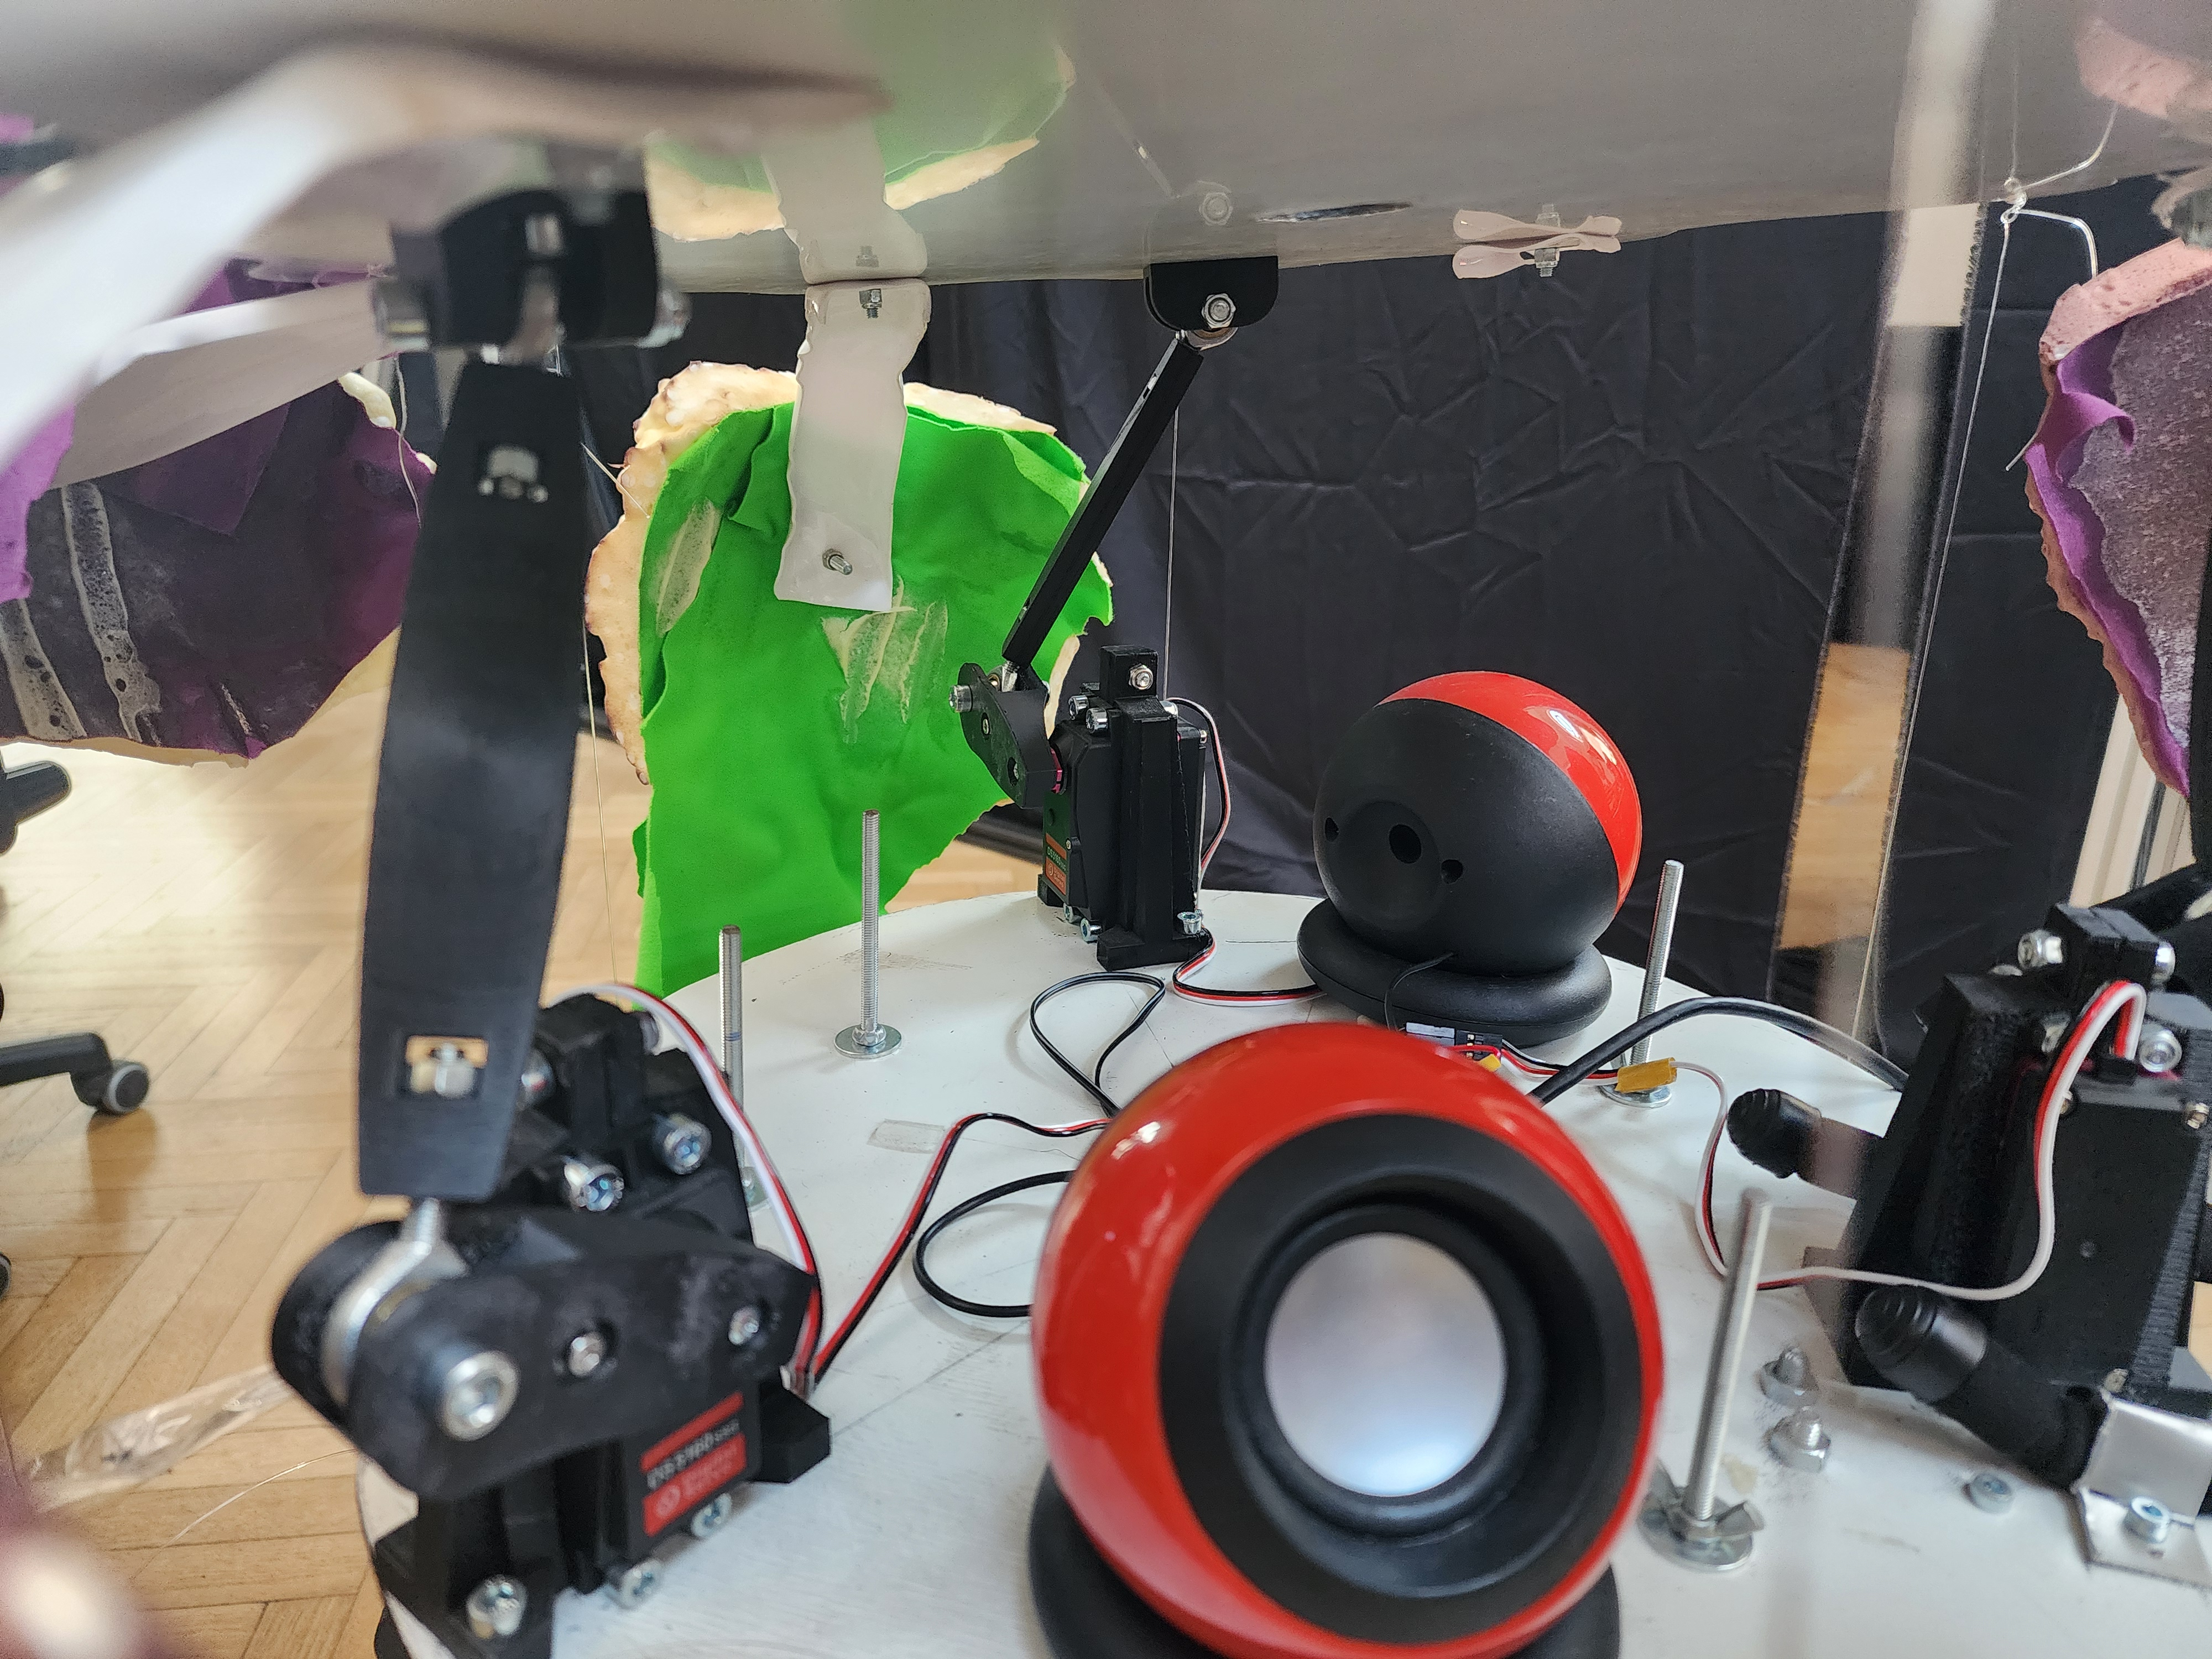
\includegraphics[width=\textwidth]{Images/NewHeadDoubleJoint (6).jpg}
        \caption{Head Arm with Rod Ends (Sway to right)}
        \label{fig:head_arm_rod_end_right}
    \end{minipage}
    \hfill
    \begin{minipage}{0.45\textwidth}
        \centering
        \includegraphics[width=\textwidth]{Images/NewHeadDoubleJoint (2).jpg}
        \caption{Head Arm with Rod Ends (Sway to left)}
        \label{fig:head_arm_rod_end_left}
    \end{minipage}
\end{figure}

Structural strength analysis demonstrates significant improvement in mechanical robustness and load-bearing capability while accepting reduced precision during stationary periods due to joint flexibility. The trade-off provides enhanced durability and operational reliability for social robot applications.

Load capacity testing validates the enhanced design's capability to handle operational loads without component failure or excessive wear. Longevity testing demonstrates sustained performance under extended operational scenarios typical of social robot research applications, though some plastic degradation becomes visible over extended periods while maintaining functional operation.

\subsection{Hybrid Construction Approach}

The final implementation combines 3D printed structural components with metal heim joints to achieve optimal balance between cost, performance, and maintainability.

\subsubsection{Material Selection and Integration}

The hybrid approach utilizes 3D printed PLA components for structural framework elements where weight and cost optimization provide system benefits. Metal heim joints provide superior performance at critical articulation points where durability and precision requirements exceed plastic capabilities.

Integration methodology ensures proper mechanical connection between printed and metal components through threaded interfaces and proper mechanical attachment techniques. Interface design accommodates thermal expansion differences and provides secure long-term connection.

Cost optimization through selective material usage maintains reasonable component costs while providing enhanced performance where critical to system operation. The approach enables high-performance characteristics without excessive cost impact on the overall system.

\section{Camera Integration and Mounting Solutions}

The camera integration system addresses the unique challenges of mounting sophisticated sensing equipment within Tino's soft fabric structure while maintaining the robot's aesthetic appeal and operational capabilities.

\begin{figure}[H]
    \centering
    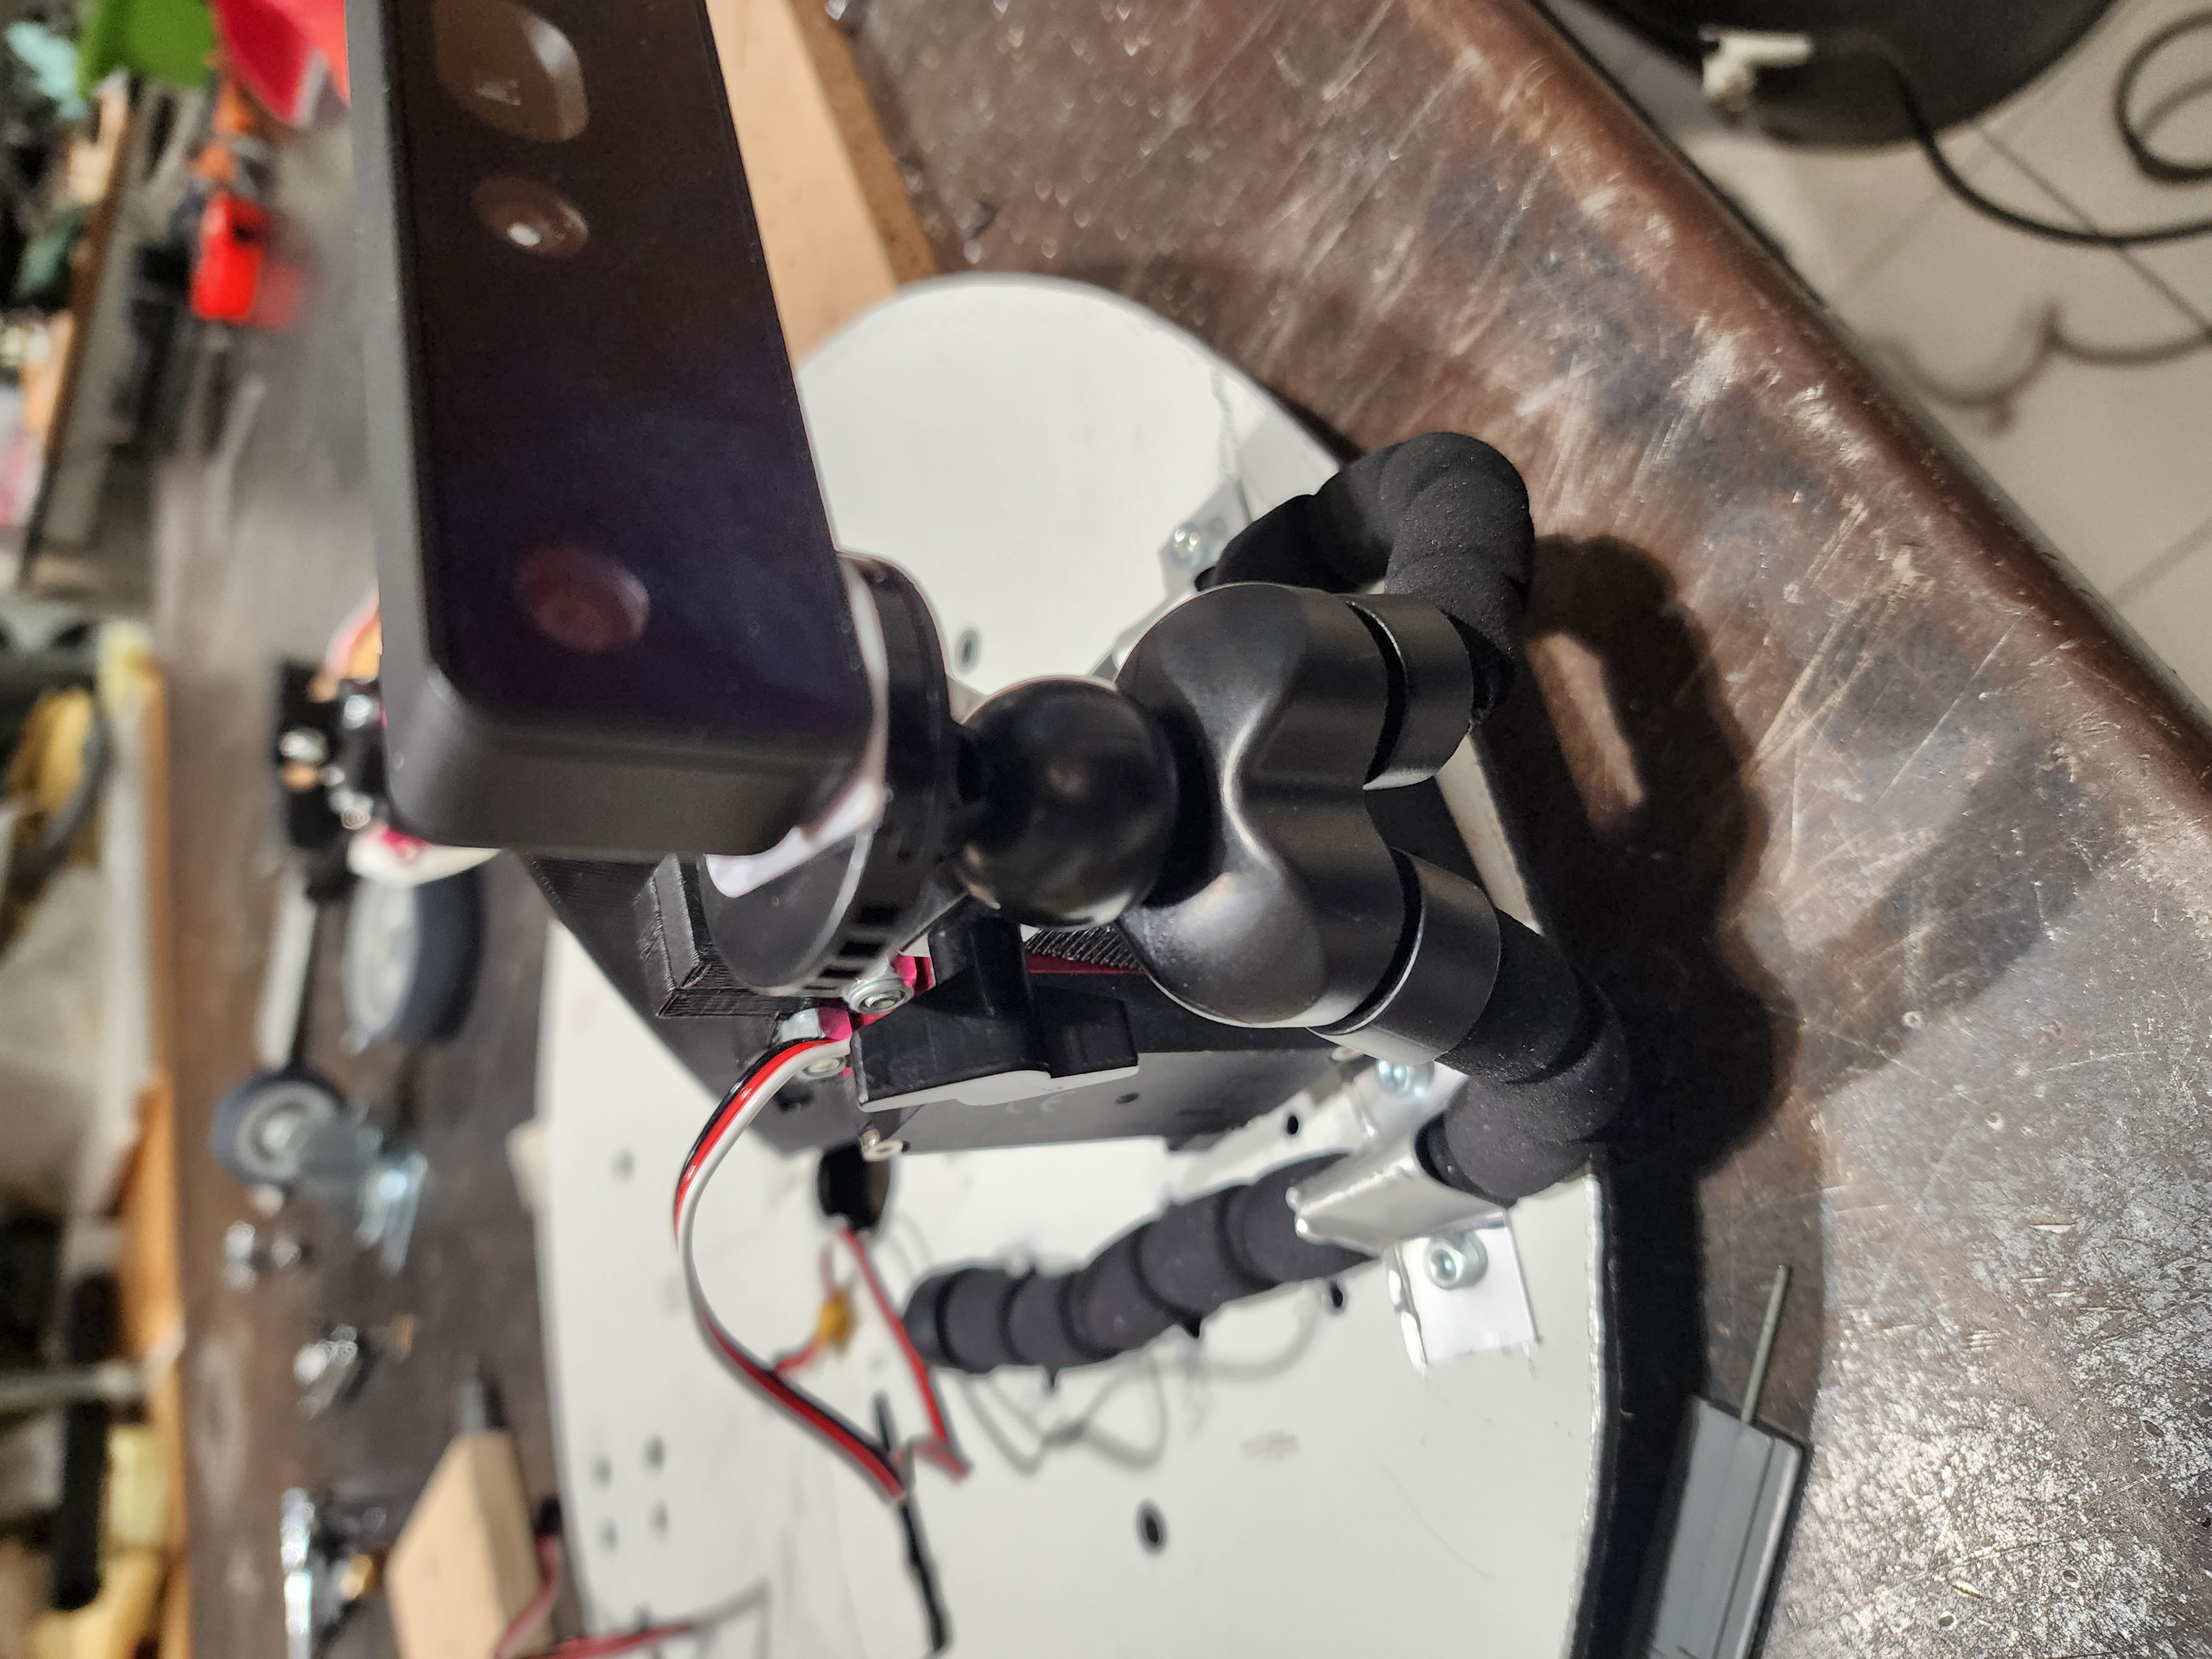
\includegraphics[width=0.6\textwidth, angle=-90]{Images/TripodOnHeadCamera.jpg}
    \caption{Oak-D Pro Camera Mounted on Tripod System}
    \label{fig:tripod_camera_mount}
\end{figure}

\subsection{Mounting System Design and Mechanical Integration}

The camera mounting system provides stable support for the Oak-D Pro camera while integrating with Tino's existing Stewart platform head mechanism and fabric covering system.

\subsubsection{Tripod-Based Support System Development}

The tripod mounting system utilizes simple brackets to create a fixed and stable camera support that eliminates the flexibility and vibration issues encountered with the original Raspberry Pi camera mount. Bracket design prioritizes rigidity while maintaining compatibility with the existing servo head structure.

Mechanical stability analysis demonstrates significant improvement in camera positioning stability compared to the flexible original mount that exhibited excessive movement during robot operation. Static deflection testing validates adequate stiffness for high-quality image acquisition during movement.

The camera mounting system operates independently from the Stewart platform head mechanism, providing dedicated stable positioning for the Oak-D Pro camera without mechanical coupling to head movements. This independent mounting ensures camera stability regardless of head articulation.

\begin{figure}[H]
    \centering
    \begin{minipage}{0.45\textwidth}
        \centering
        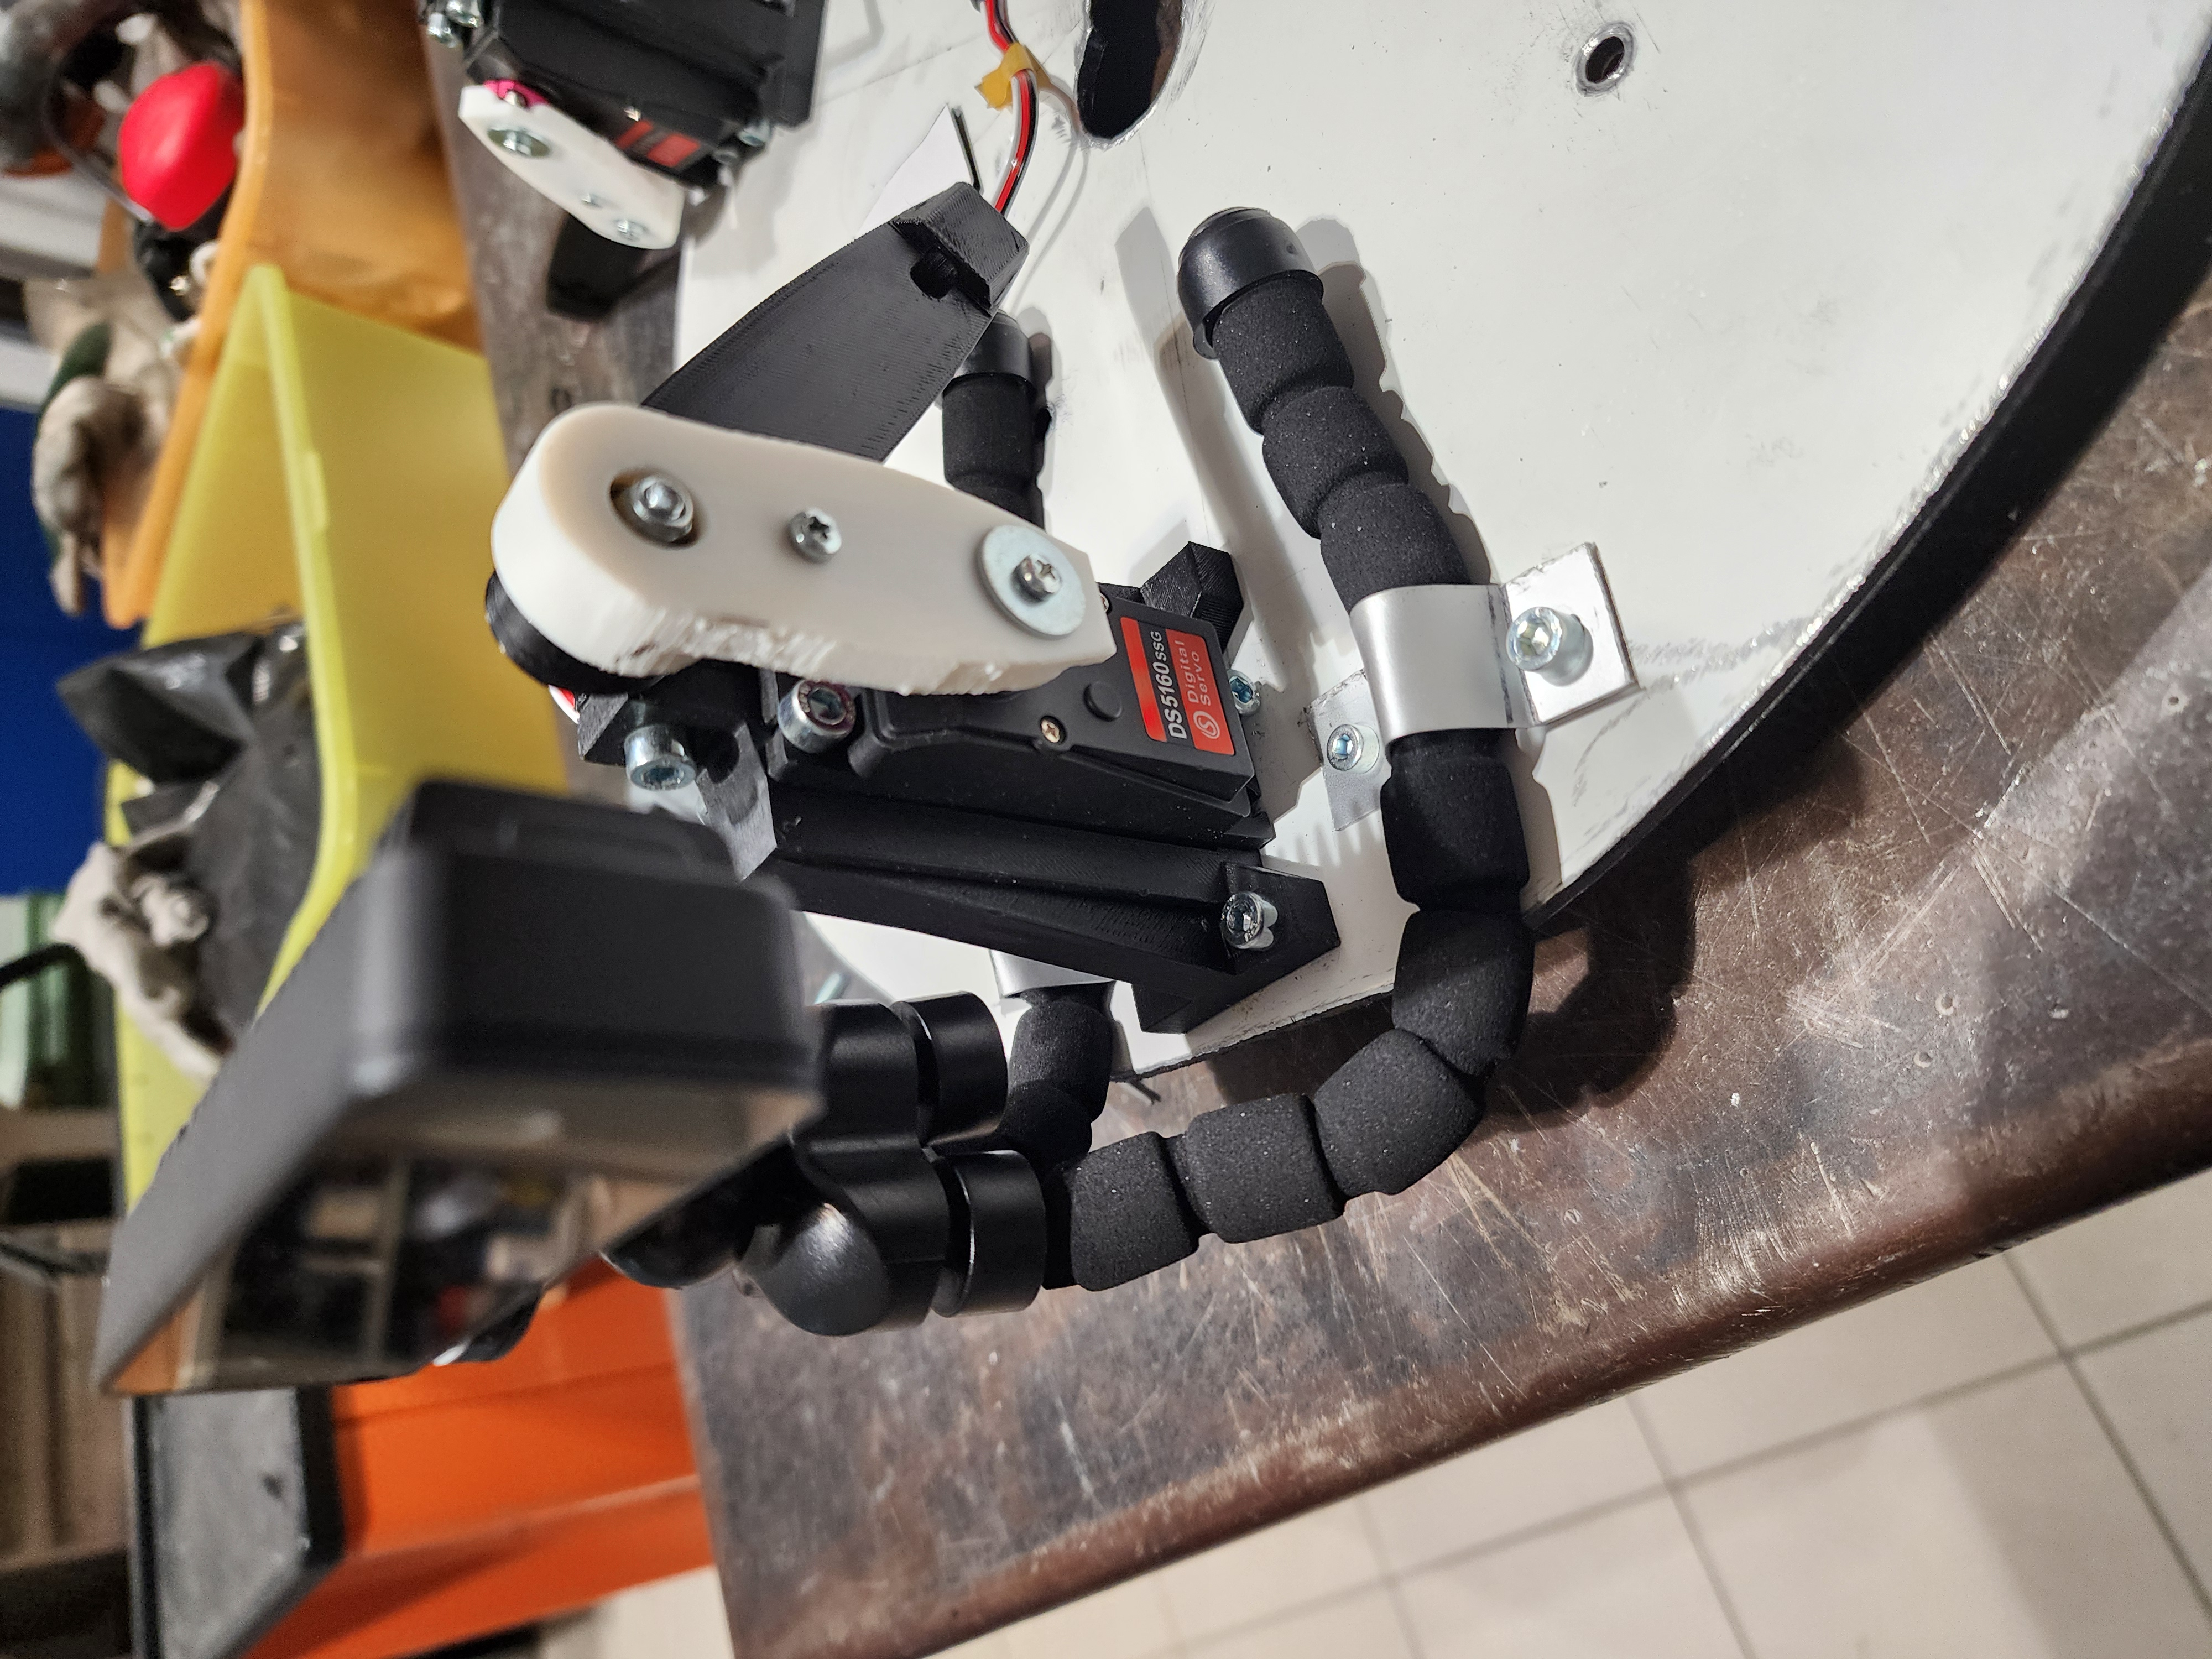
\includegraphics[width=\textwidth, angle=-90]{Images/TripodOnHeadCamera (3).jpg}
        \caption{Oak-D Pro Camera Mounted on Tripod System (Side View)}
        \label{fig:tripod_camera_mount_side}
    \end{minipage}
    \hfill
    \begin{minipage}{0.45\textwidth}
        \centering
        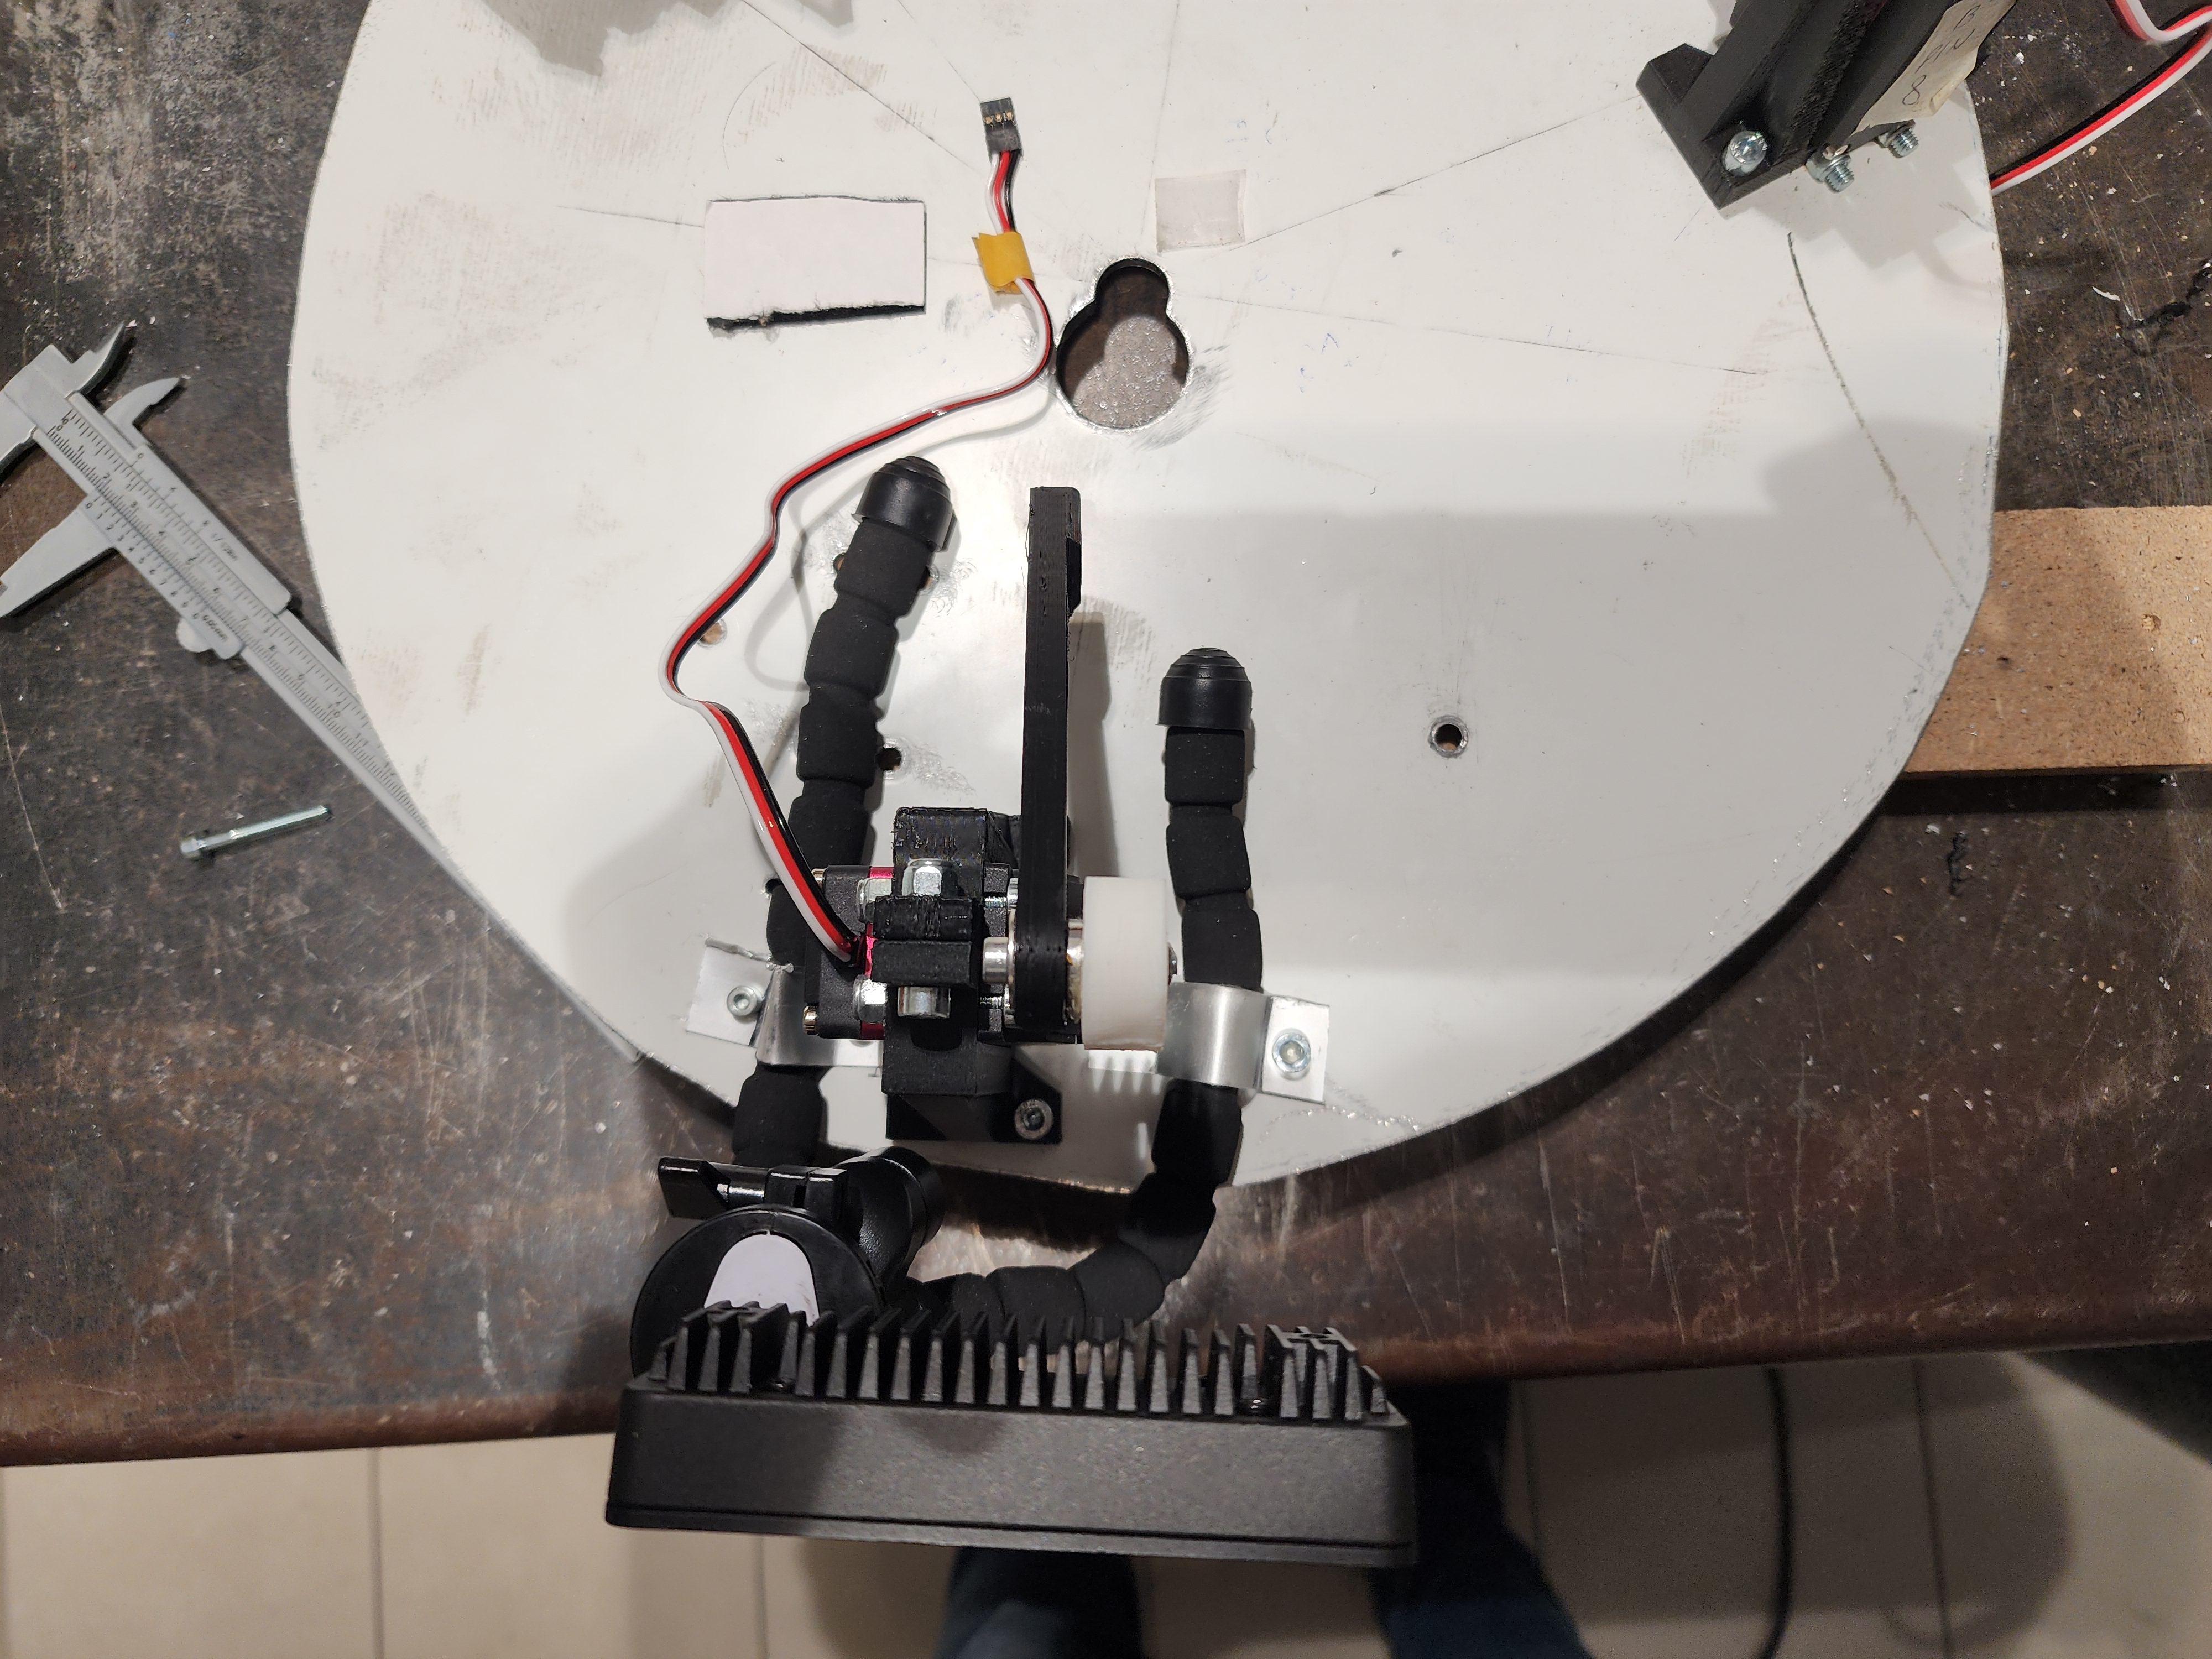
\includegraphics[width=\textwidth]{Images/TripodOnHeadCamera (2).jpg}
        \caption{Oak-D Pro Camera Mounted on Tripod System (Top View)}
        \label{fig:tripod_camera_mount_top}
    \end{minipage}
\end{figure}

\subsubsection{Structural Compatibility and Integration Challenges}

The mounting system accommodates the existing servo head geometry while providing secure attachment points for the Oak-D Pro camera. Geometric constraints required custom bracket design that works within the available space while providing adequate support.

Weight distribution analysis ensures that camera addition does not compromise Stewart platform performance or exceed servo motor capabilities. Camera weight integration maintains head balance characteristics while providing enhanced sensing capabilities.

Mechanical interfaces utilize standard mounting hardware that enables camera removal for maintenance or upgrade without requiring bracket system modification. Modular approach provides flexibility for future system enhancement while maintaining operational reliability.

\subsection{Fabric Integration and Visibility Solutions}

The fabric integration system addresses the fundamental challenge of maintaining camera visibility while preserving Tino's fabric aesthetic and protecting sensitive camera components.
\begin{figure}[H]
    \centering
    \begin{minipage}{0.45\textwidth}
        \centering
        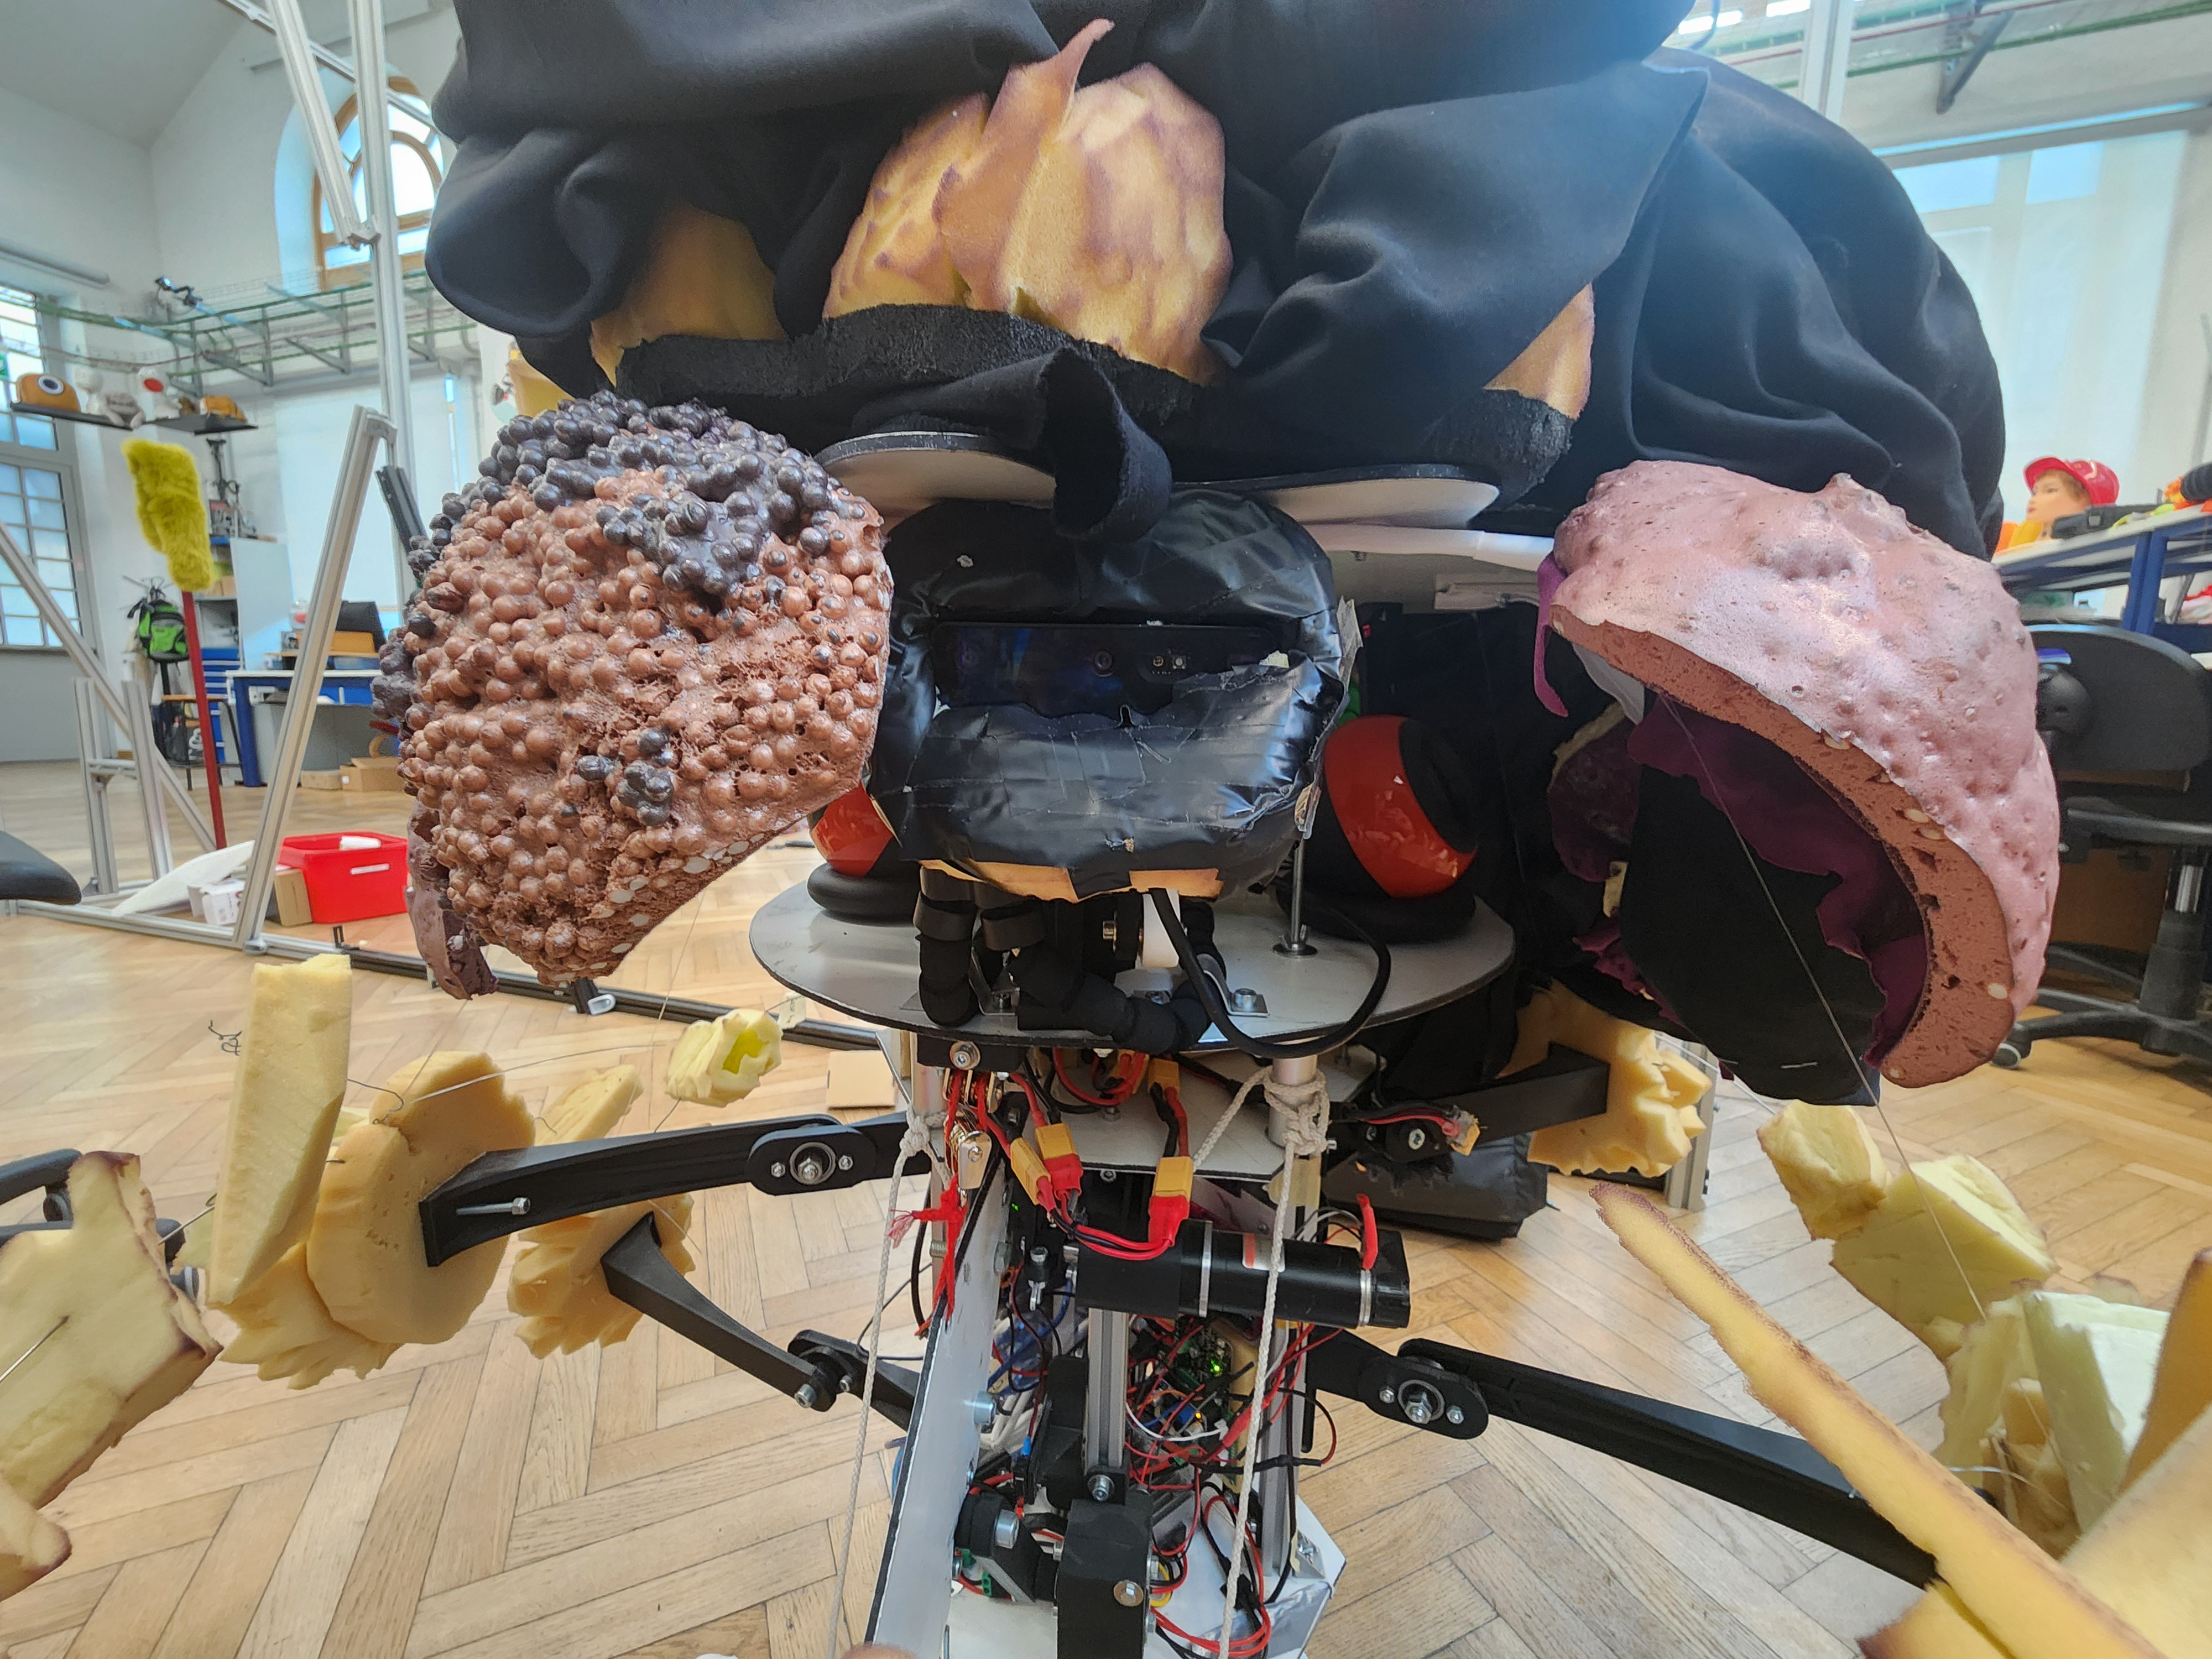
\includegraphics[width=\textwidth]{Images/FirstTryCameraHiding.jpg}
        \caption{Initial Camera Concealment Attempt (Front View)}
        \label{fig:first_try_camera_hiding}
    \end{minipage}
    \hfill
    \begin{minipage}{0.45\textwidth}
        \centering
        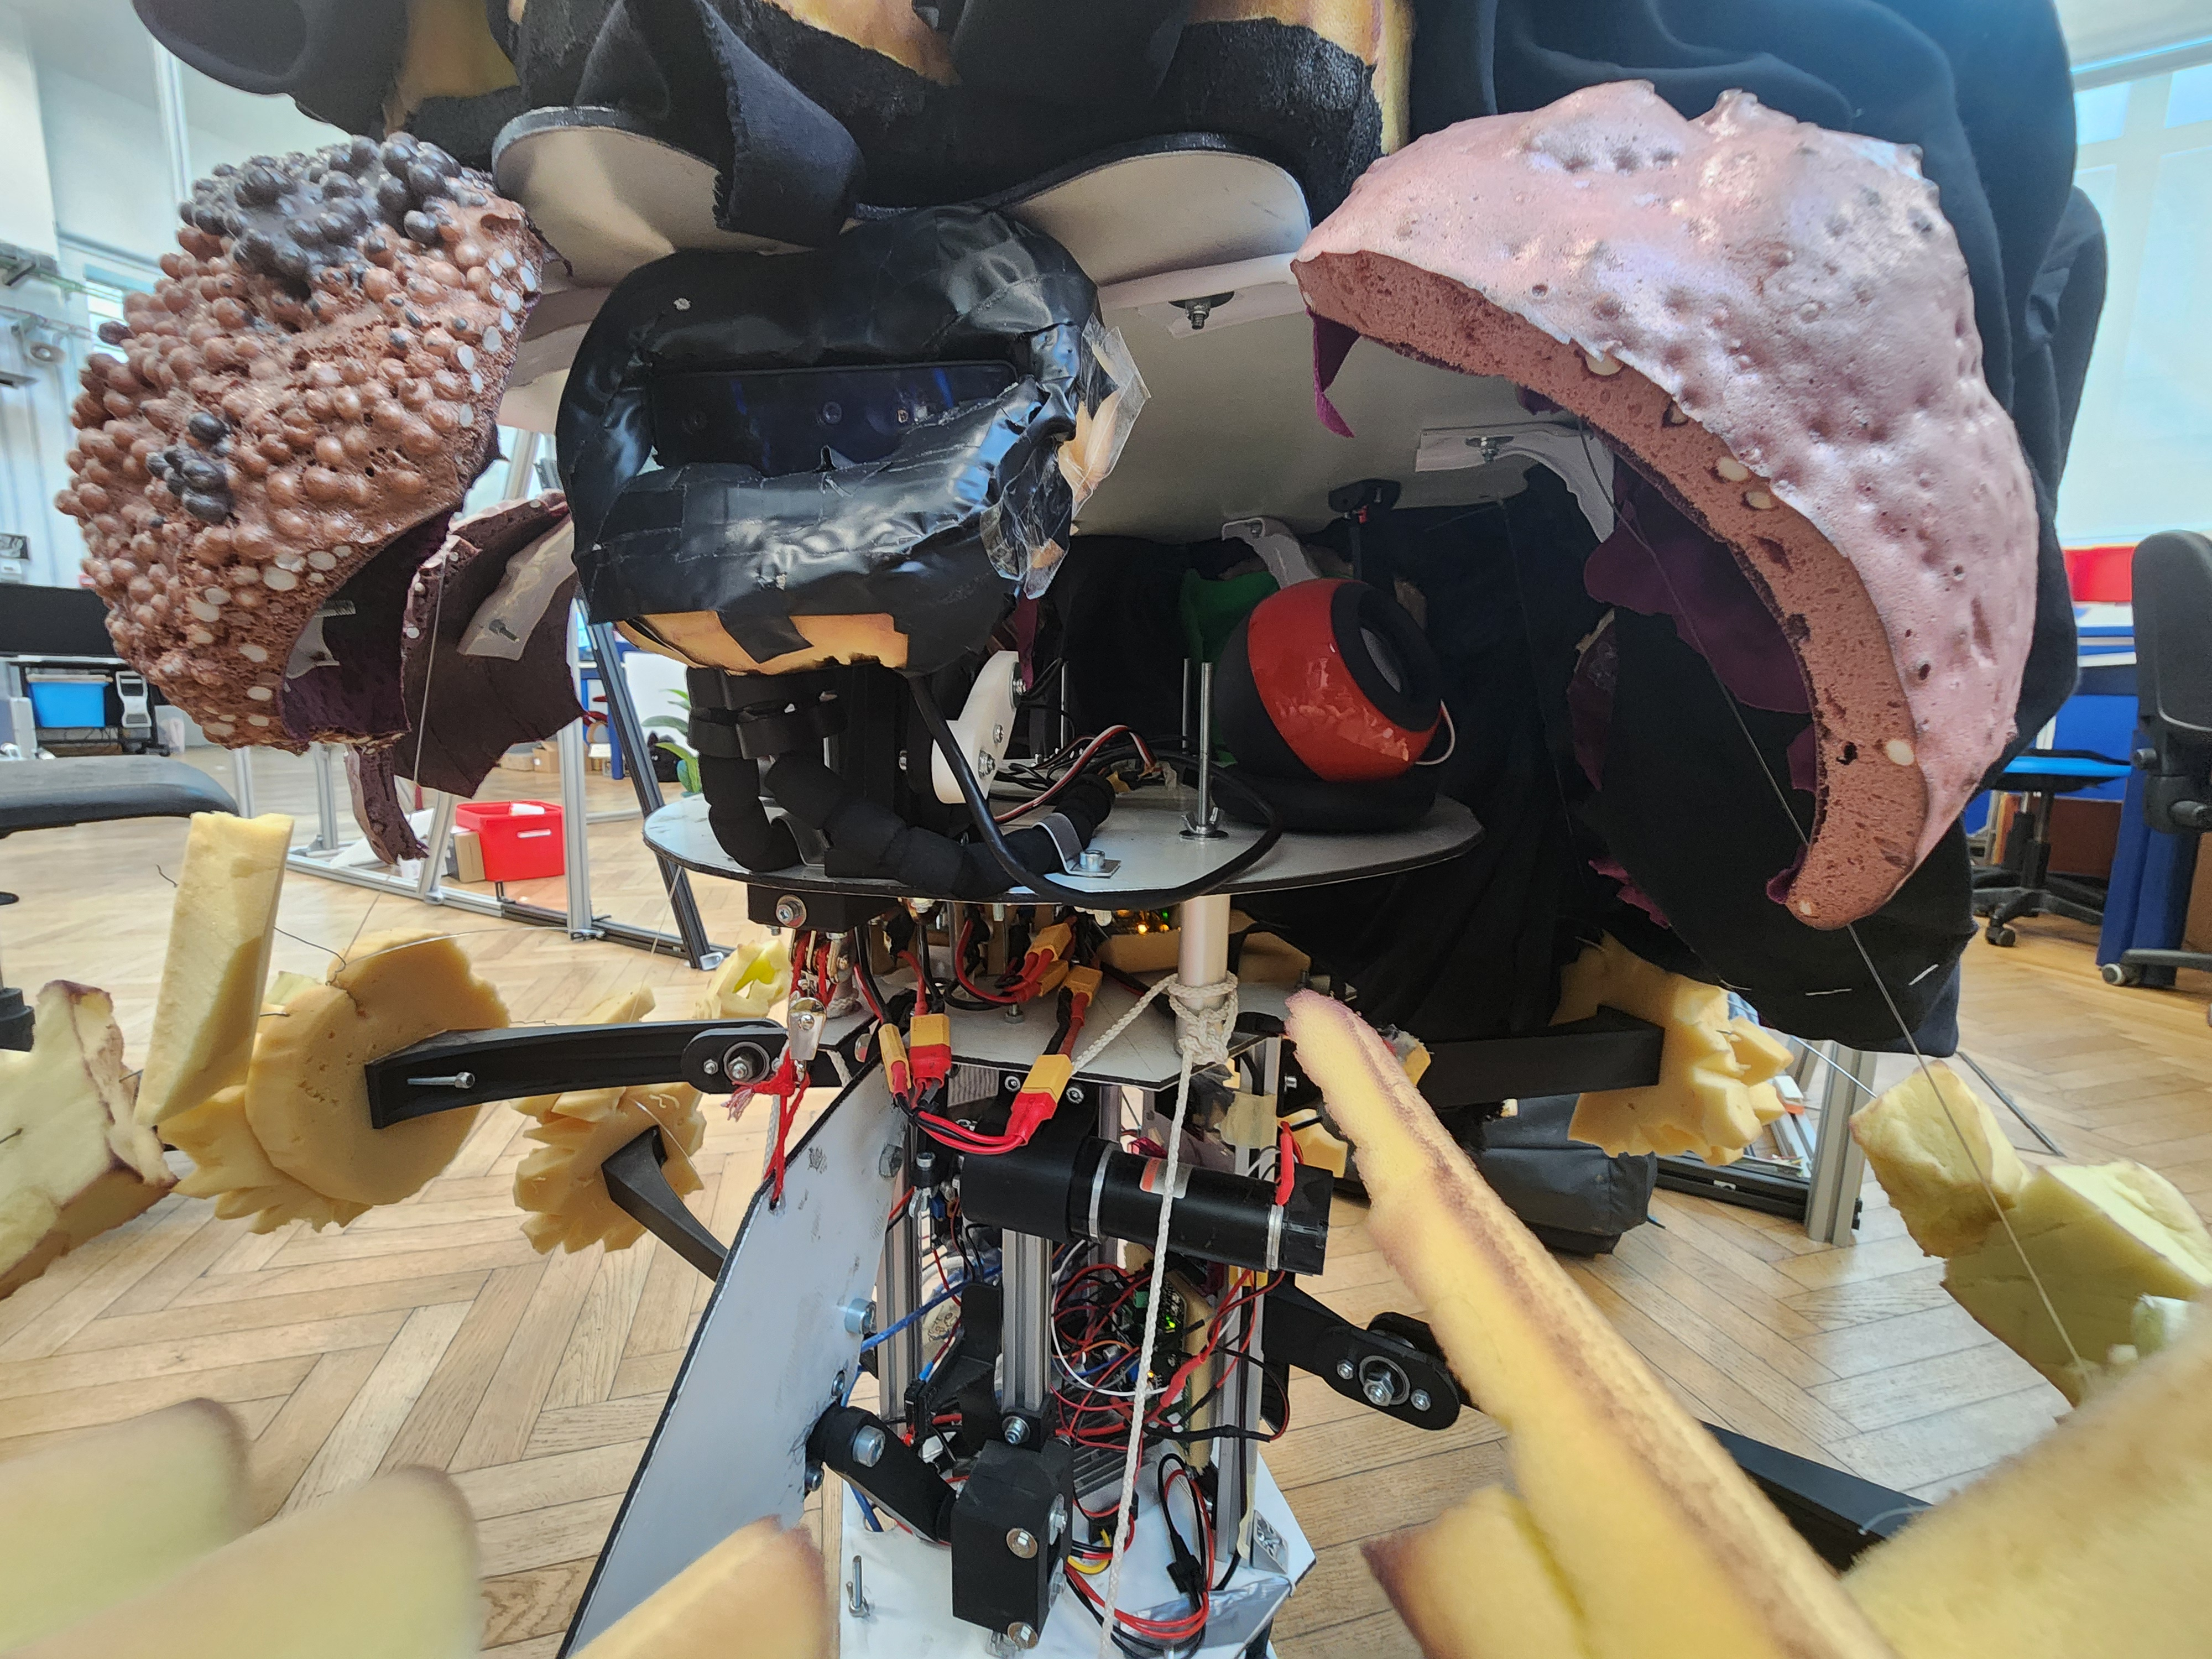
\includegraphics[width=\textwidth]{Images/FirstTryCameraHiding (3).jpg}
        \caption{Initial Camera Concealment Attempt (Side View)}
        \label{fig:camera_hiding_mesh}
    \end{minipage}
\end{figure}

\subsubsection{Fabric Modification and Positioning Strategies}

Fabric positioning strategies prevent interference with camera sensing while maintaining the robot's aesthetic integrity. Positioning solutions accommodate fabric movement during robot operation without compromising camera field of view or image quality.

Velcro attachment systems provide secure fabric positioning that prevents fabric drift into camera field of view during operational periods. Attachment point selection utilizes strategic locations that maintain fabric appearance while providing reliable position control.

Testing procedures validate fabric positioning effectiveness under various operational scenarios including head movement, robot locomotion, and extended operational periods. Validation testing ensures consistent camera performance throughout typical social interaction scenarios.

\subsubsection{Camera Protection and Environmental Considerations}

Protection requirements address both physical protection from impact during social interaction and environmental protection from dust and moisture that could compromise camera operation. Protection solutions maintain camera accessibility for maintenance while providing adequate operational protection.

The protective approach balances camera protection needs against heat dissipation requirements and optical performance considerations. Protection system design ensures adequate camera cooling while preventing environmental contamination that could affect image quality.

Integration testing validates protection effectiveness while confirming maintained camera performance under operational conditions. Testing includes thermal performance evaluation and optical quality assessment under various environmental conditions.

\subsection{Camera Shell Development and Implementation}

The camera shell system provides comprehensive protection and fabric integration while maintaining optimal camera performance and heat dissipation characteristics.

\begin{figure}[H]
    \centering
    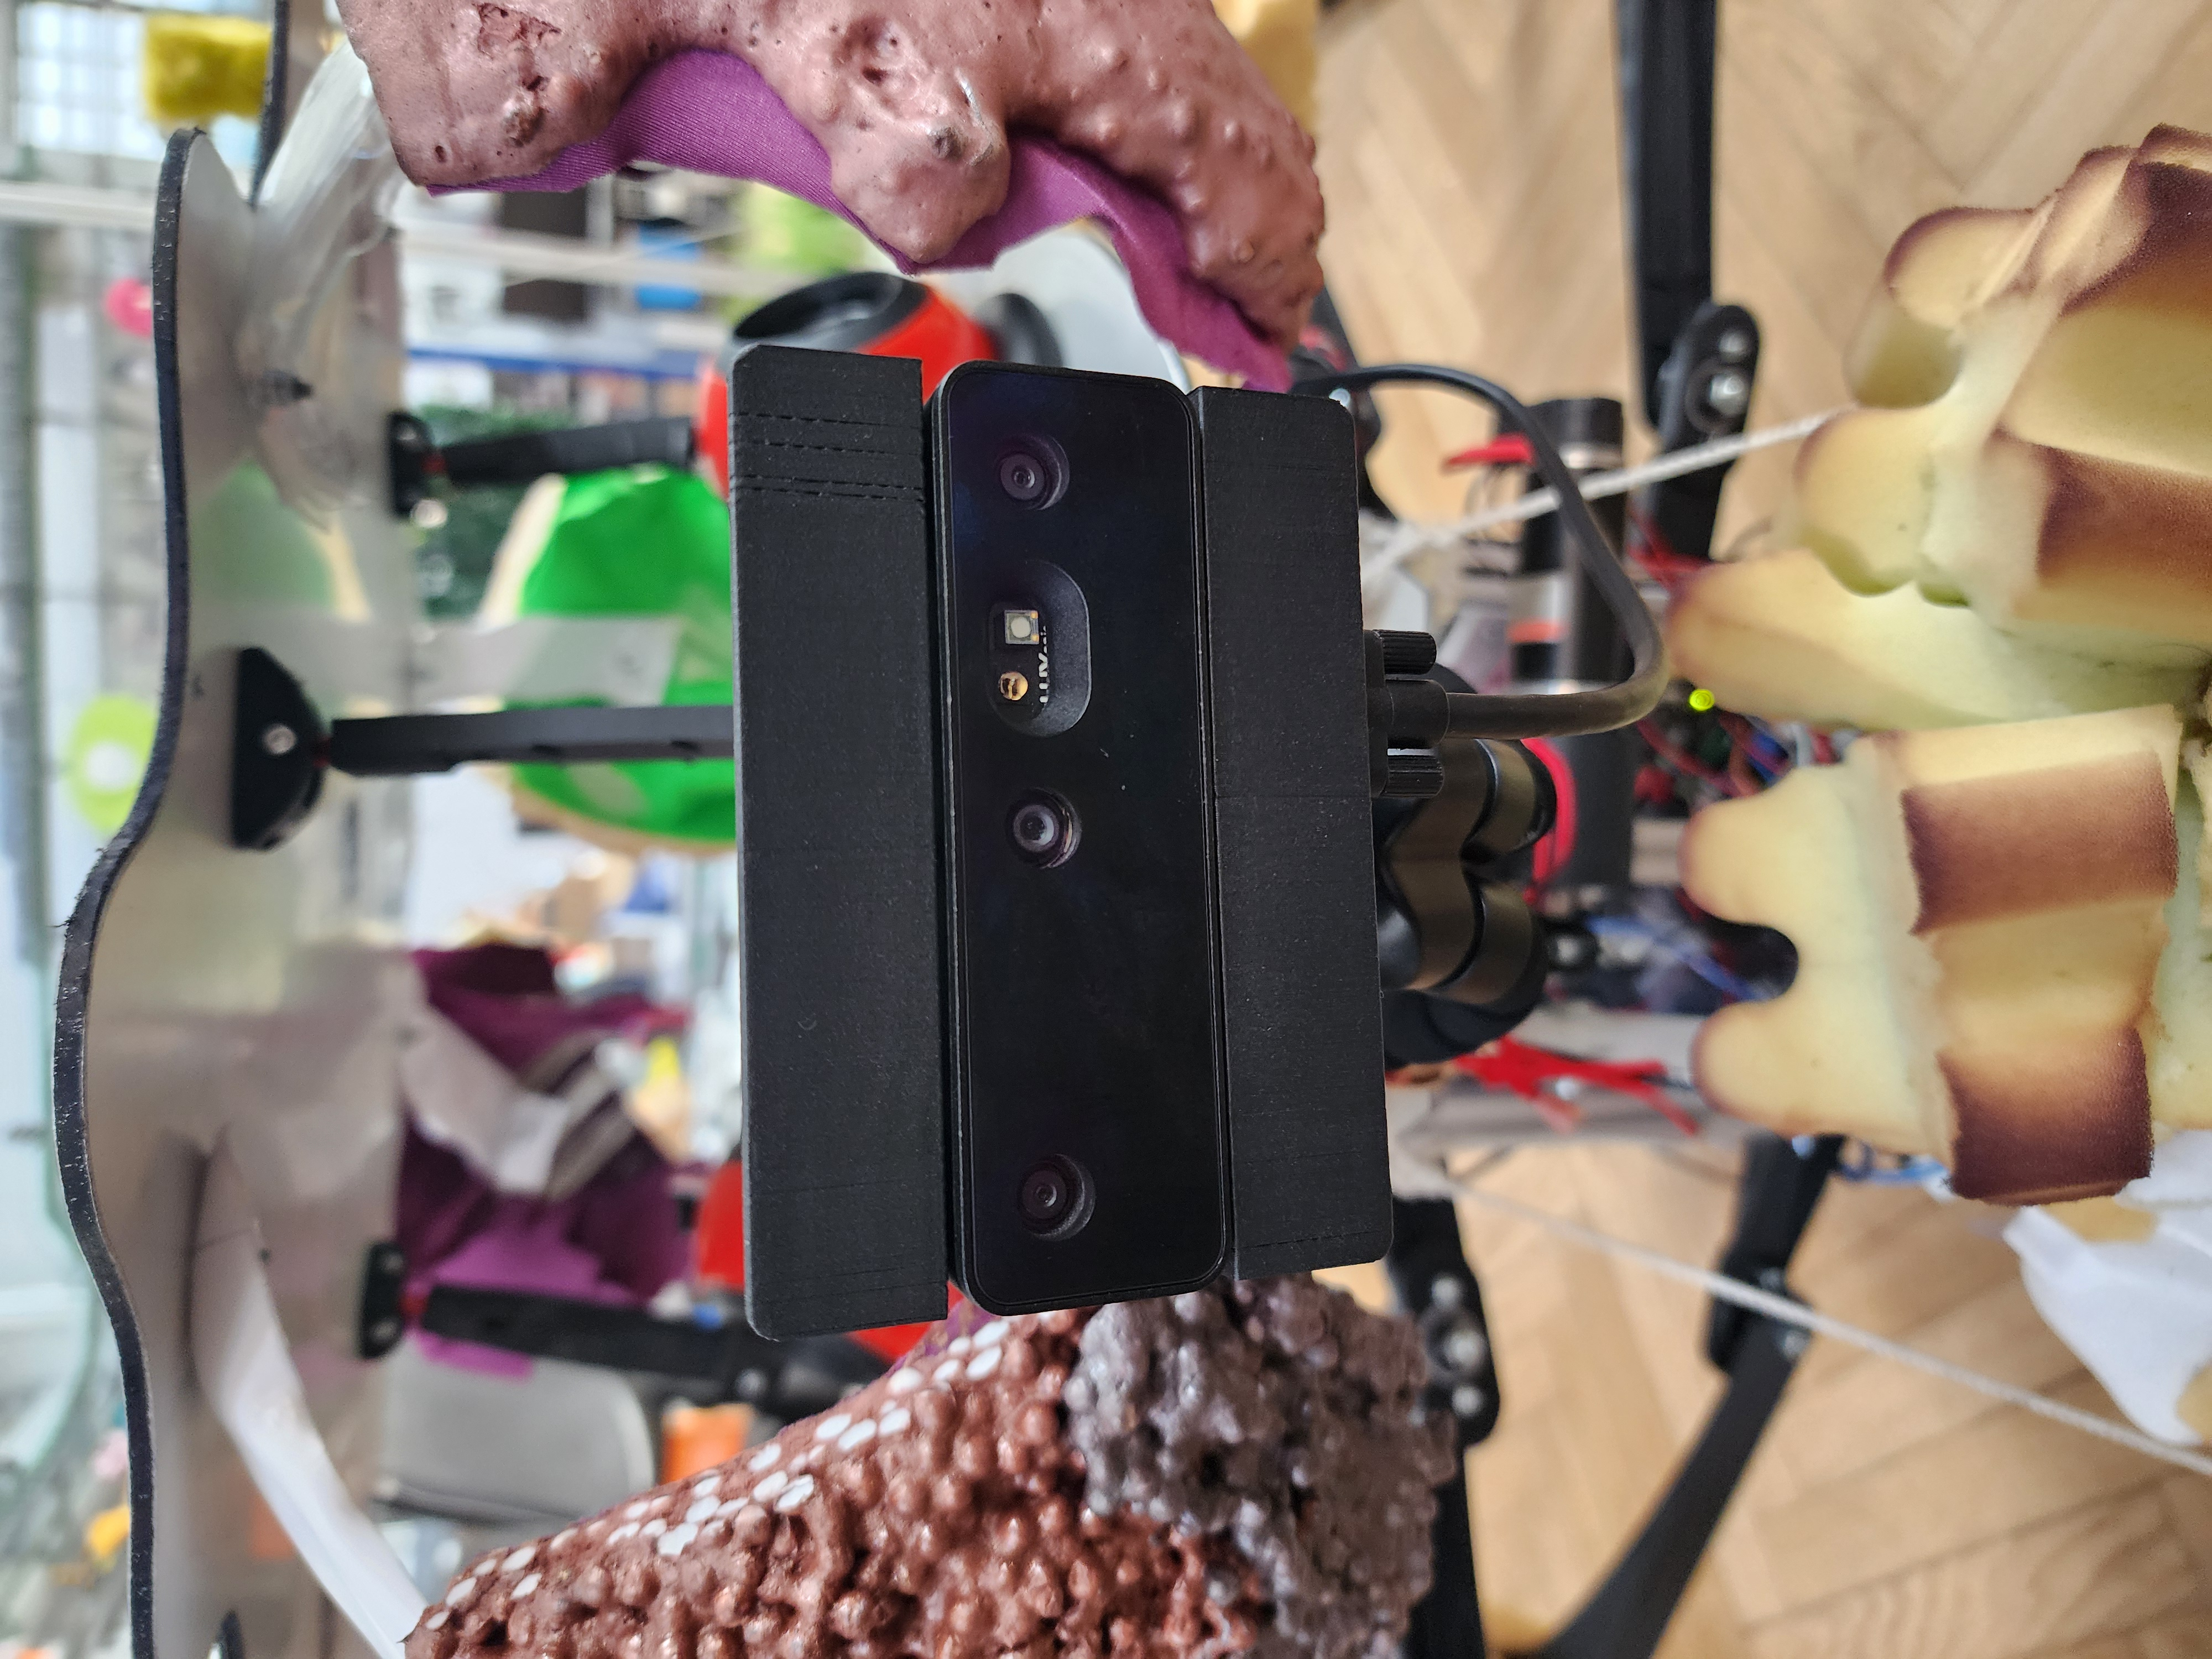
\includegraphics[height=8cm, angle=-90]{Images/CameraCasingNoMesh.jpg}
    \caption{Camera Casing without Mesh Covering}
    \label{fig:camera_casing_no_mesh}
\end{figure}

\subsubsection{Custom Enclosure Design and Functionality}

The custom shell design provides camera protection while maintaining cooling airflow through strategic ventilation openings that enable heat dissipation without compromising environmental protection. Shell geometry optimizes airflow characteristics while minimizing dust ingress.

\begin{figure}[H]
    \centering
    \begin{minipage}{0.45\textwidth}
        \centering
        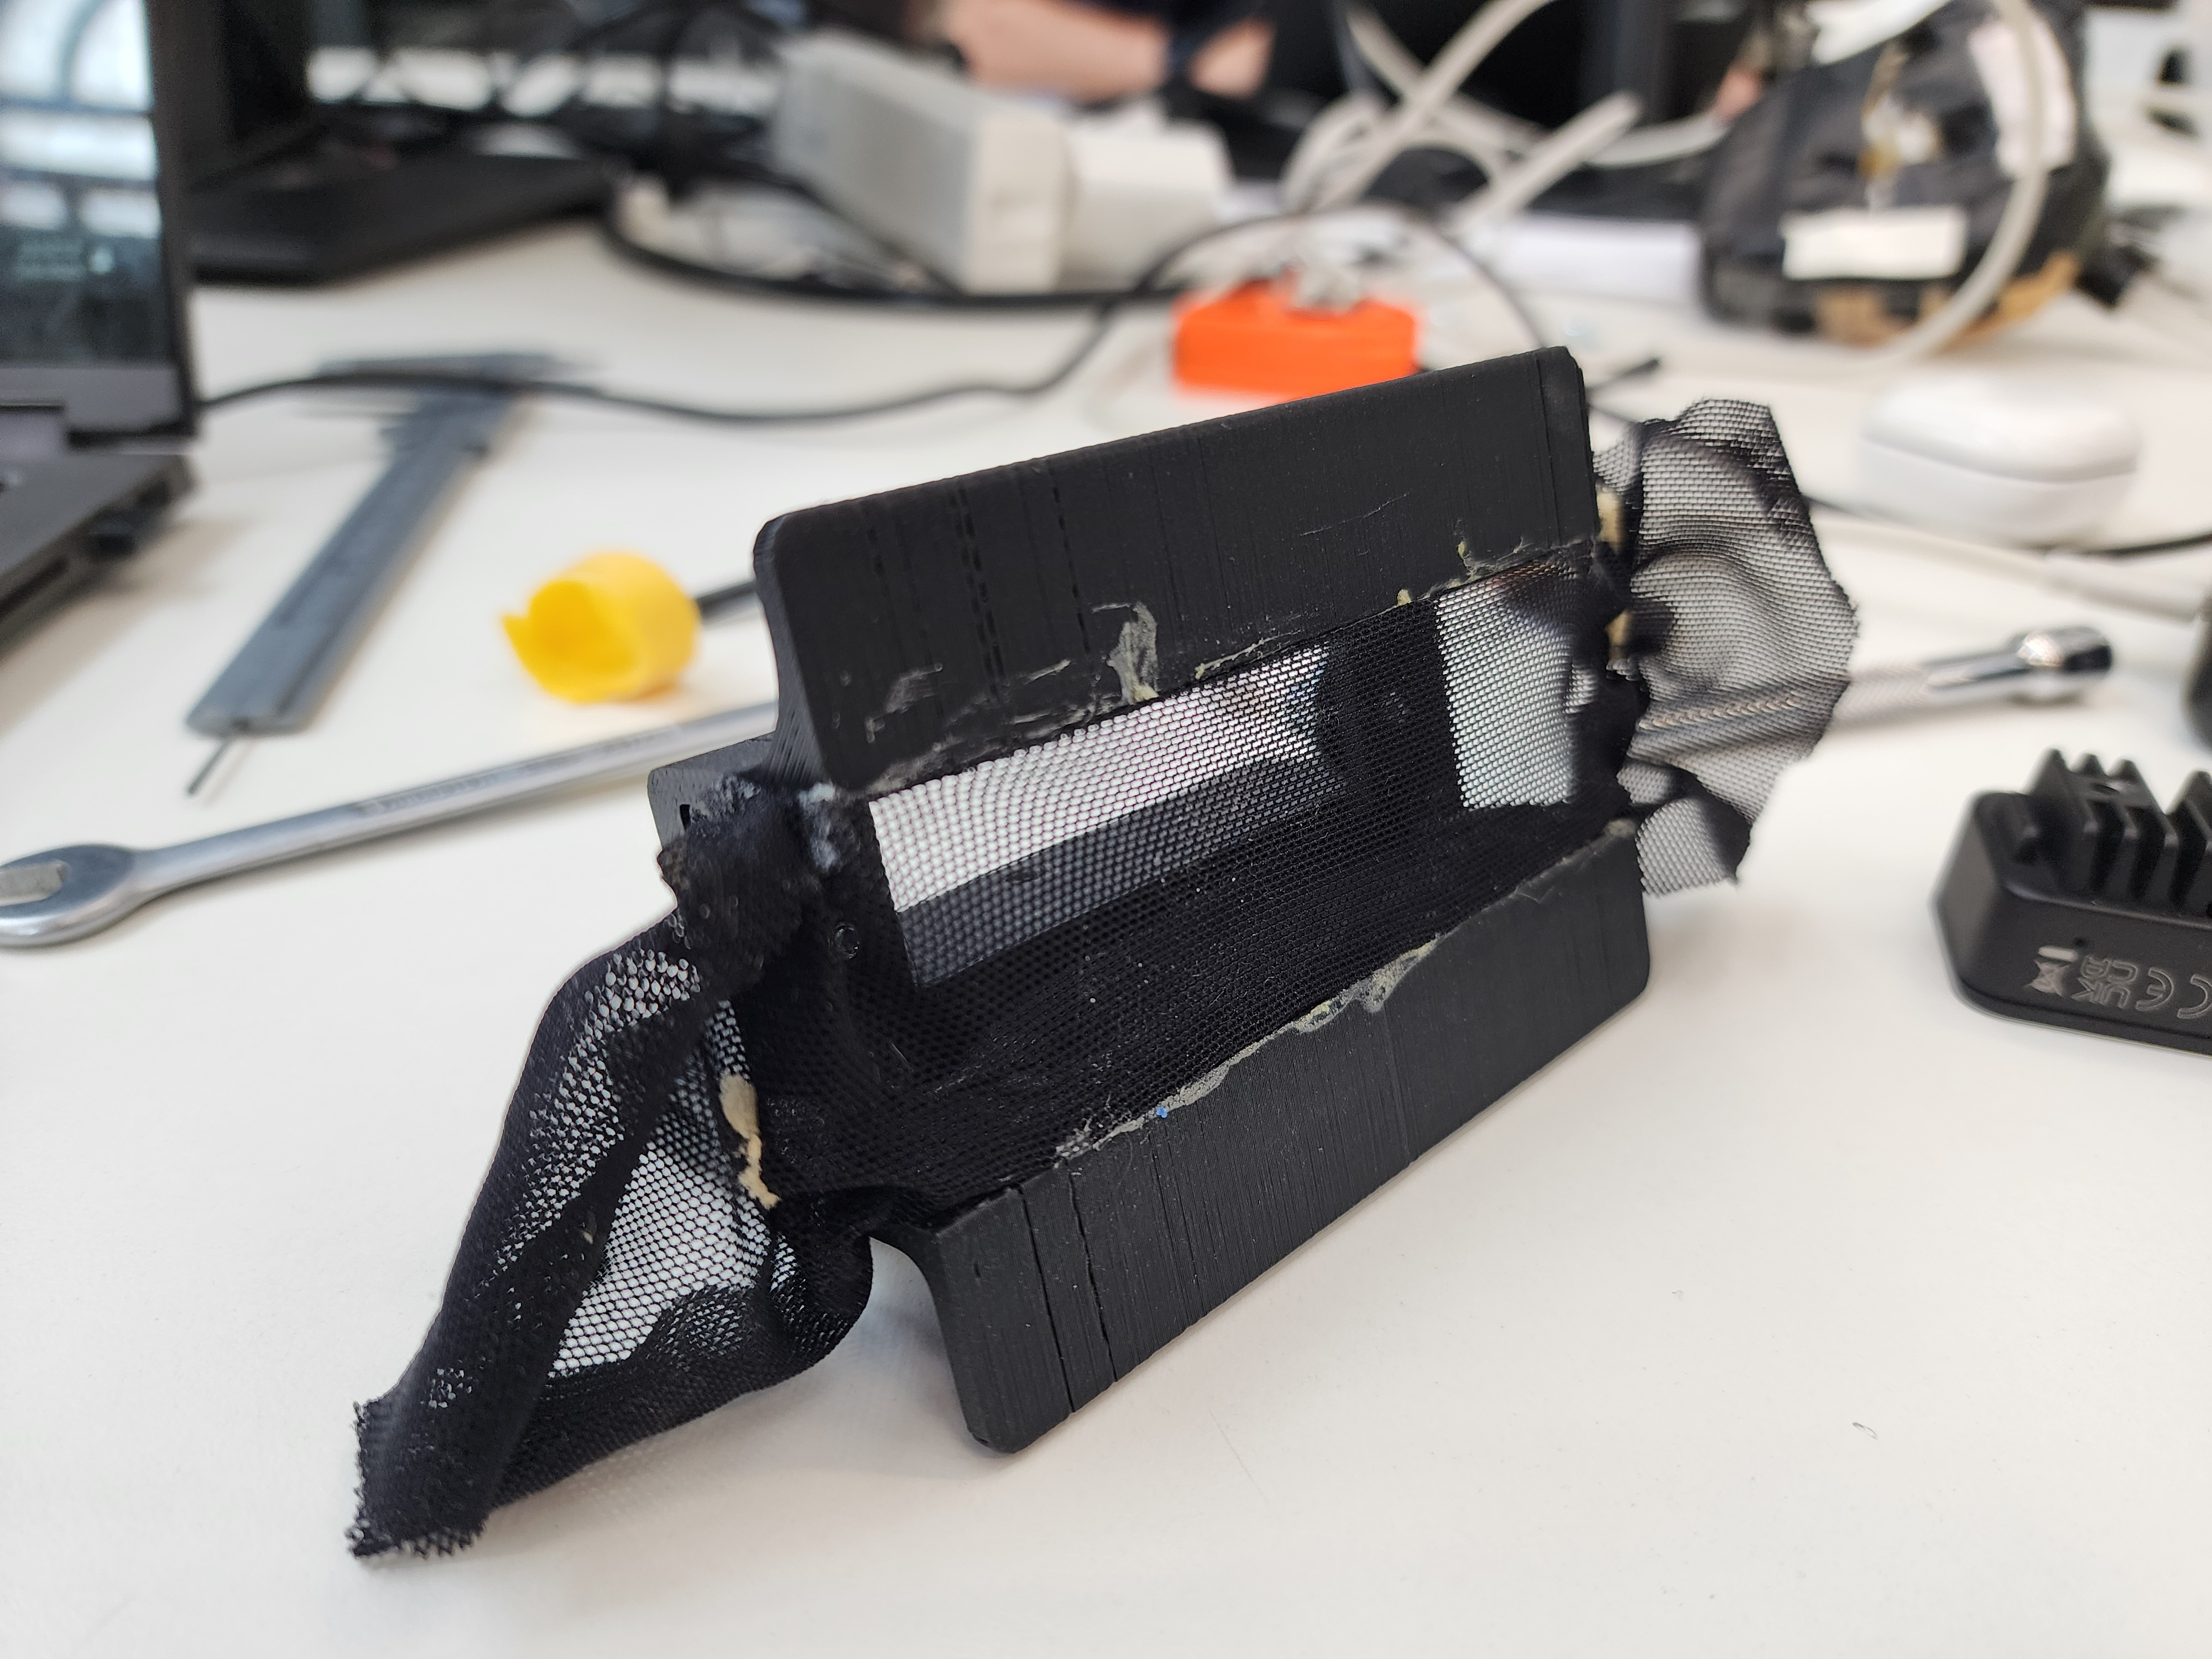
\includegraphics[width=0.8\textwidth]{Images/CameraCasingMesh.jpg}
        \caption{Camera Casing with Mesh Covering (No camera)} 
        \label{fig:camera_casing_mesh}
    \end{minipage}
    \hfill
    \begin{minipage}{0.45\textwidth}
        \centering
        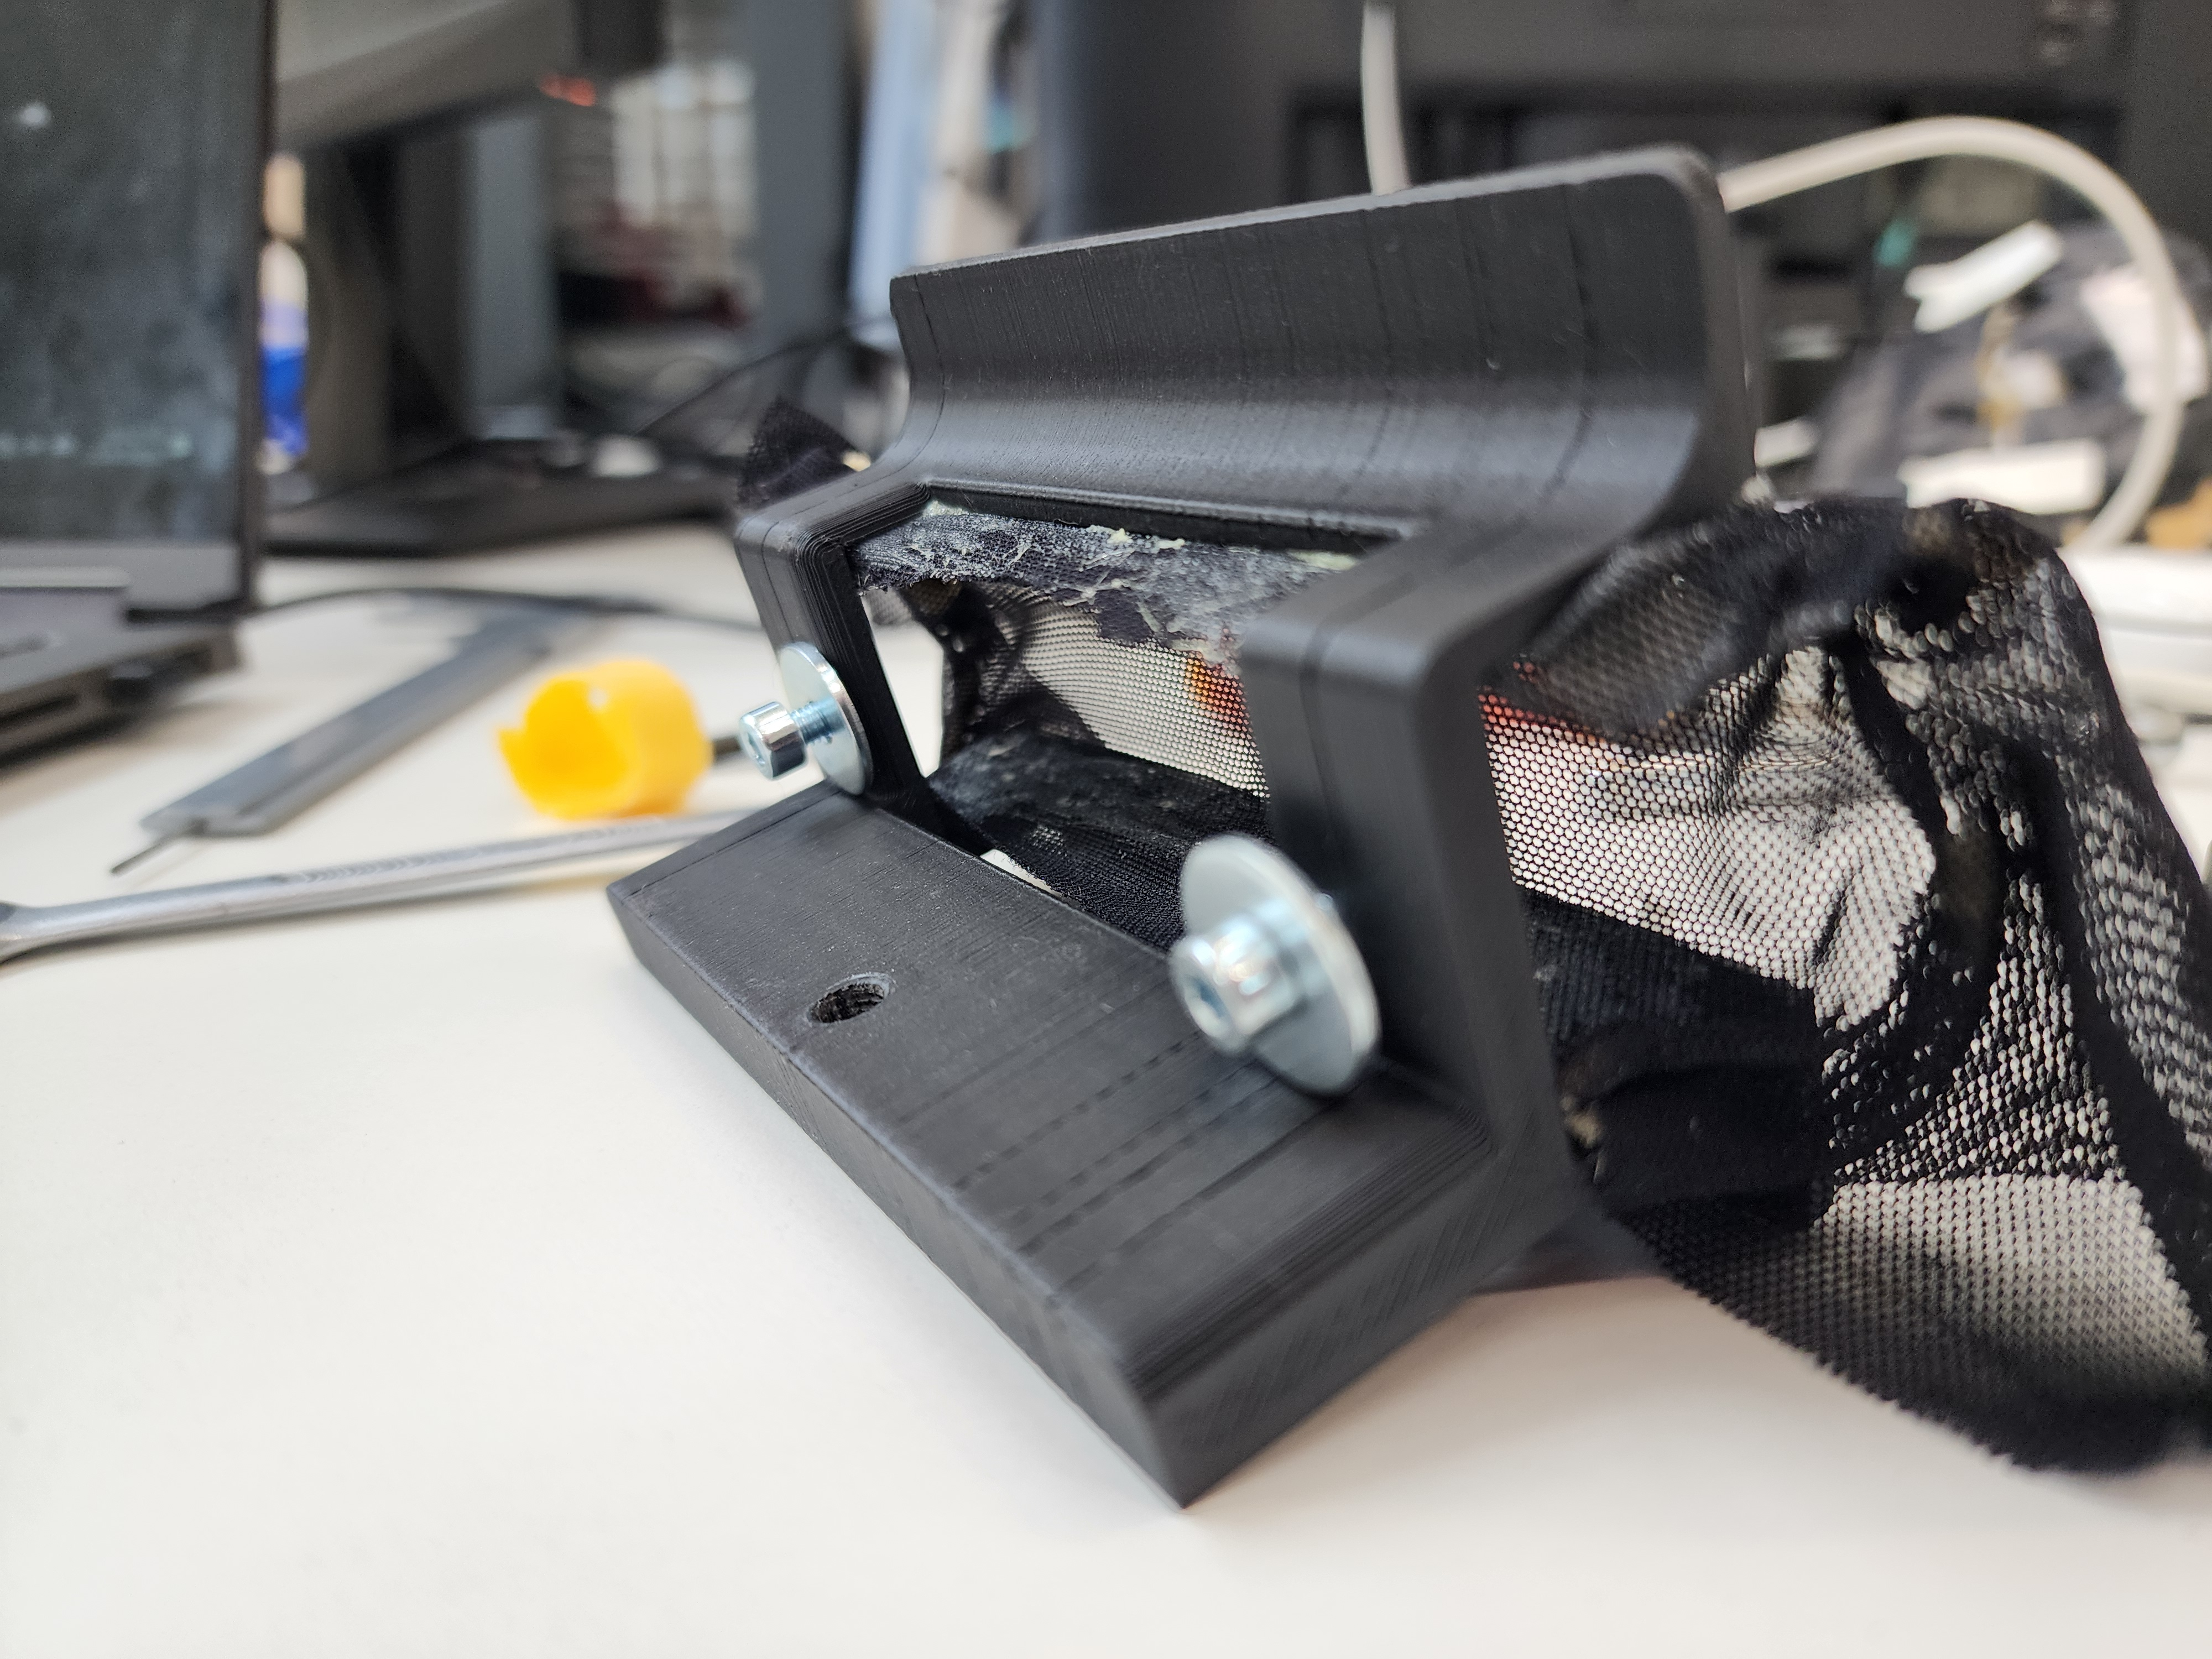
\includegraphics[width=0.8\textwidth]{Images/CameraCasingMesh (2).jpg}
        \caption{Camera Casing with Mesh Covering (No camera)}
        \label{fig:camera_casing_mesh_back}
    \end{minipage}
\end{figure}

Attachment integration with the tripod mounting system provides secure shell mounting that enables camera access for maintenance while providing operational protection. Mounting system design enables shell removal without disturbing camera alignment or calibration.

Thermal management considerations ensure adequate heat dissipation during extended operation periods, particularly during high-resolution stereo processing that generates significant thermal loads. Thermal testing validates adequate cooling under maximum operational loads.

\begin{figure}[H]
    \centering
    \begin{minipage}{0.45\textwidth}
        \centering
        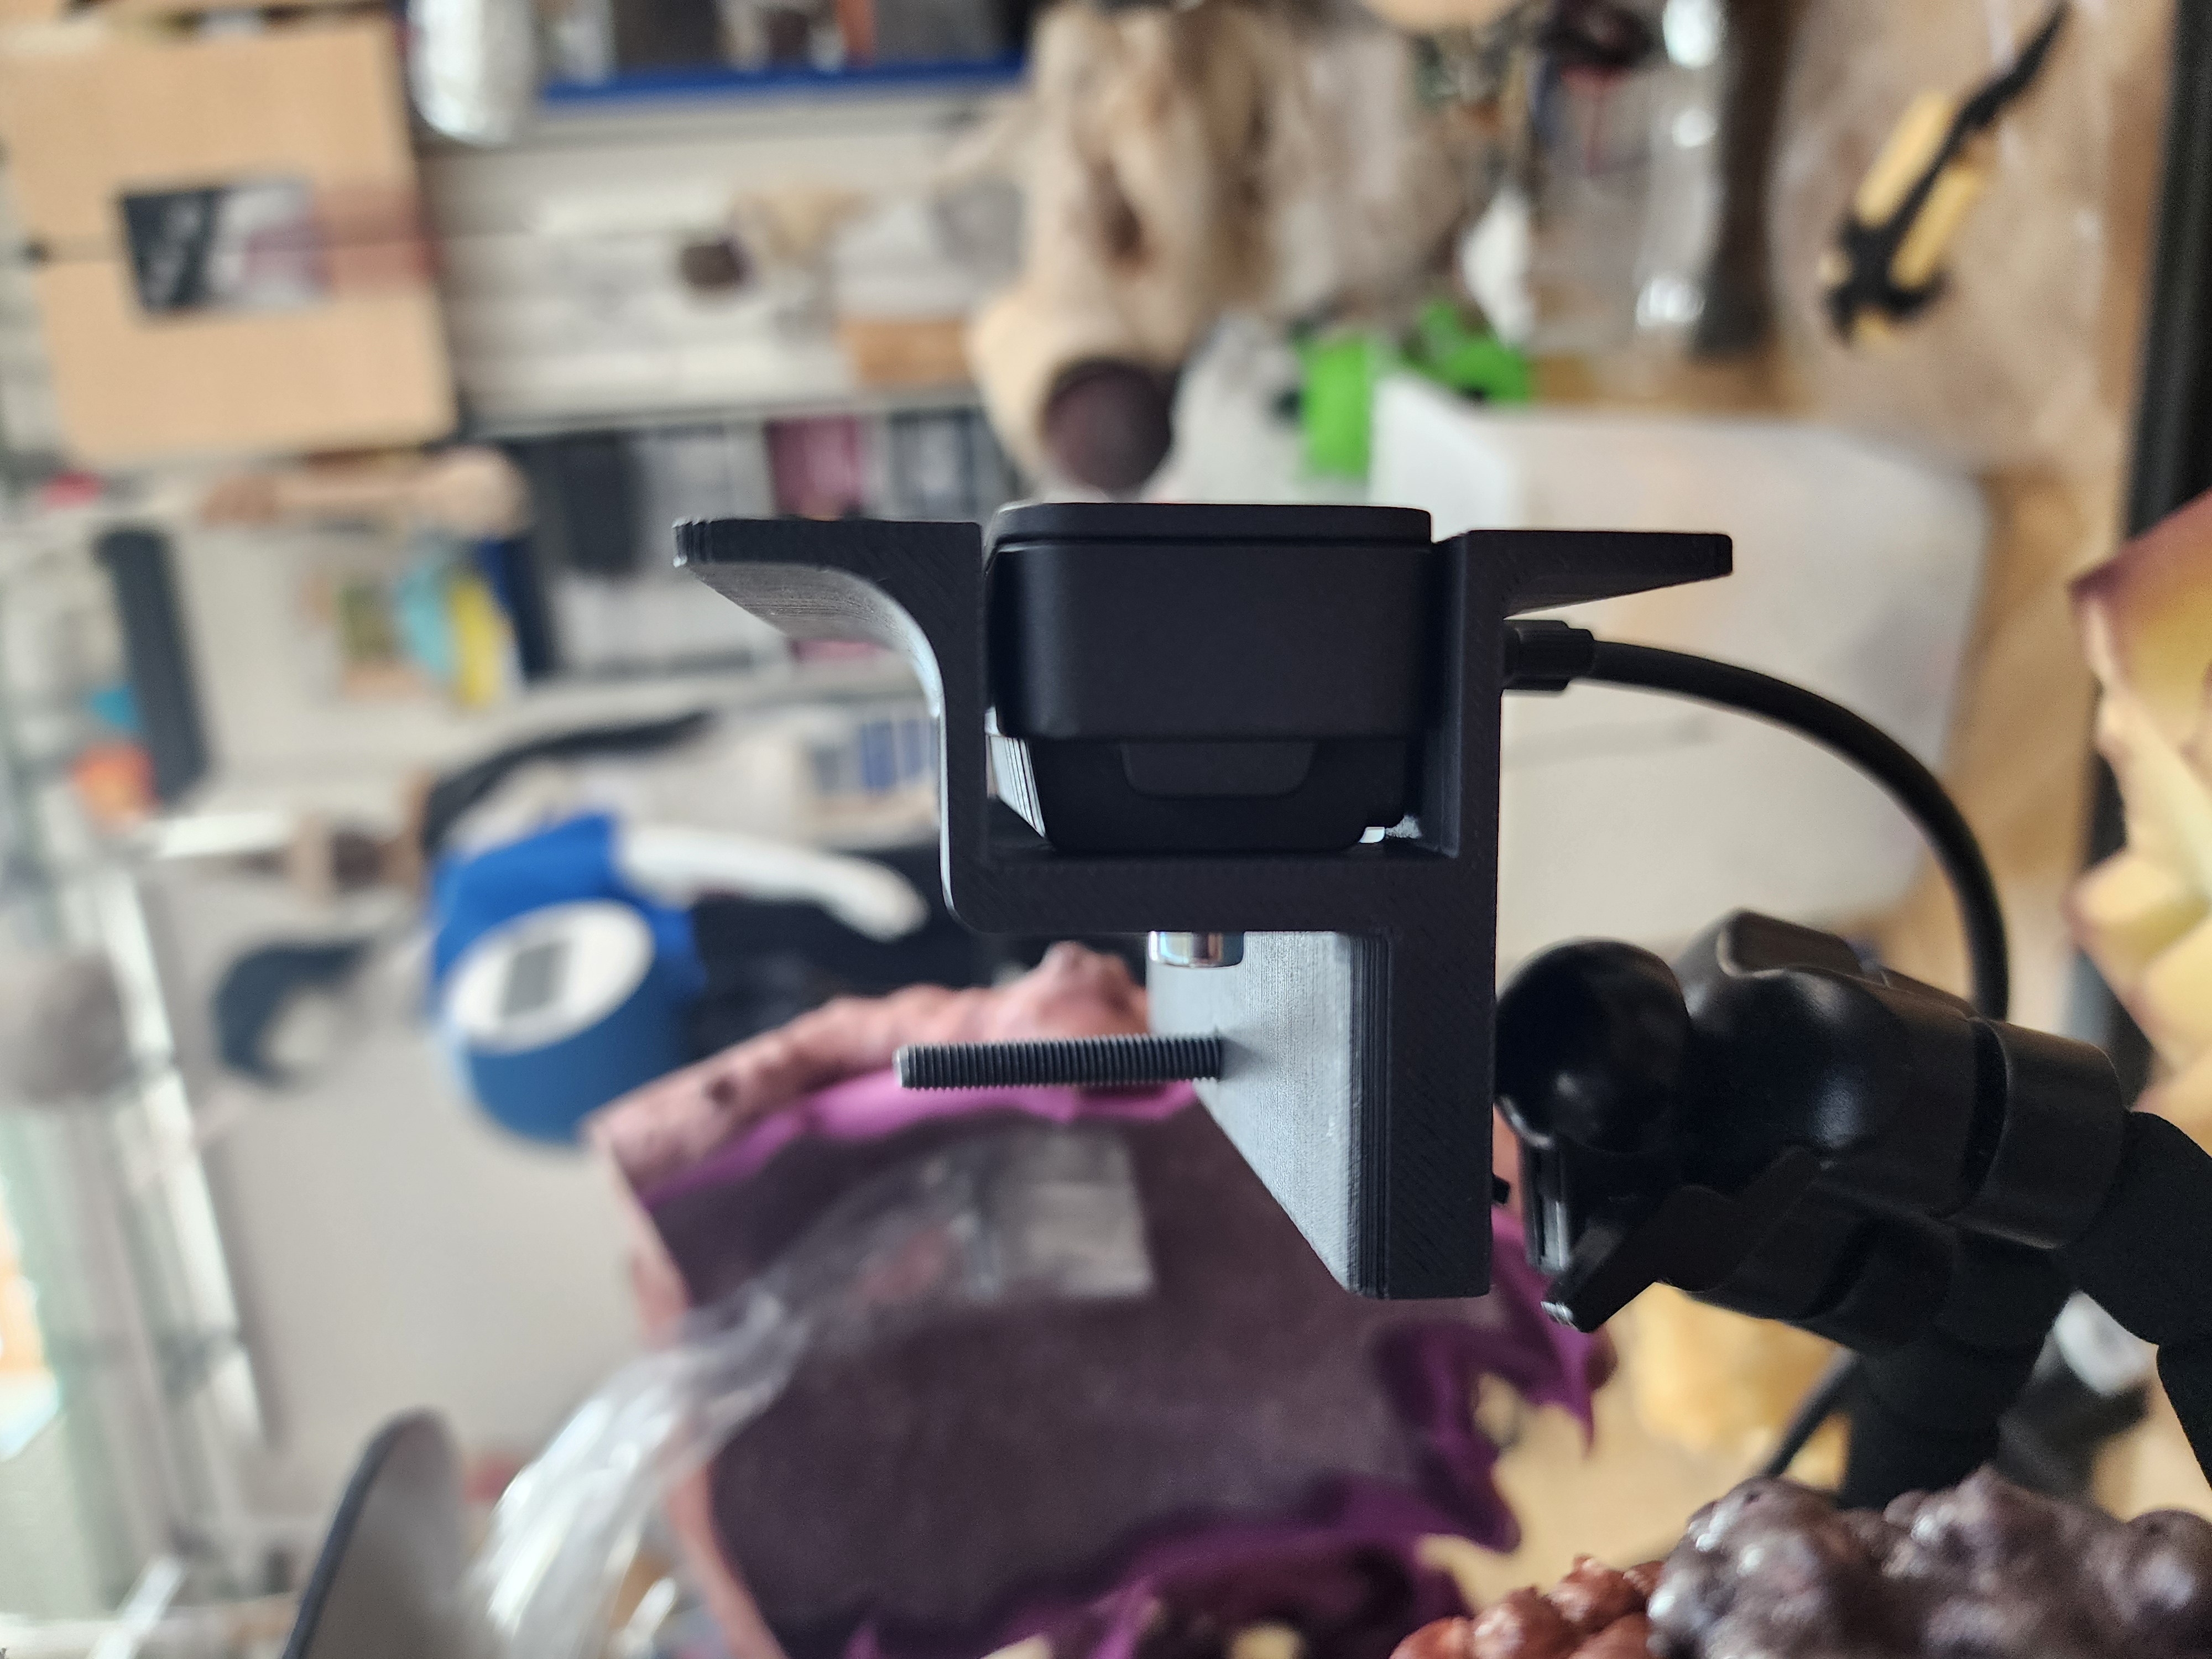
\includegraphics[width=\textwidth, angle=-90]{Images/CameraCasingNoMesh (4).jpg}
        \caption{Camera Casing without Mesh Covering (Side View)}
        \label{fig:camera_casing_no_mesh_side}
    \end{minipage}
    \hfill
    \begin{minipage}{0.45\textwidth}
        \centering
        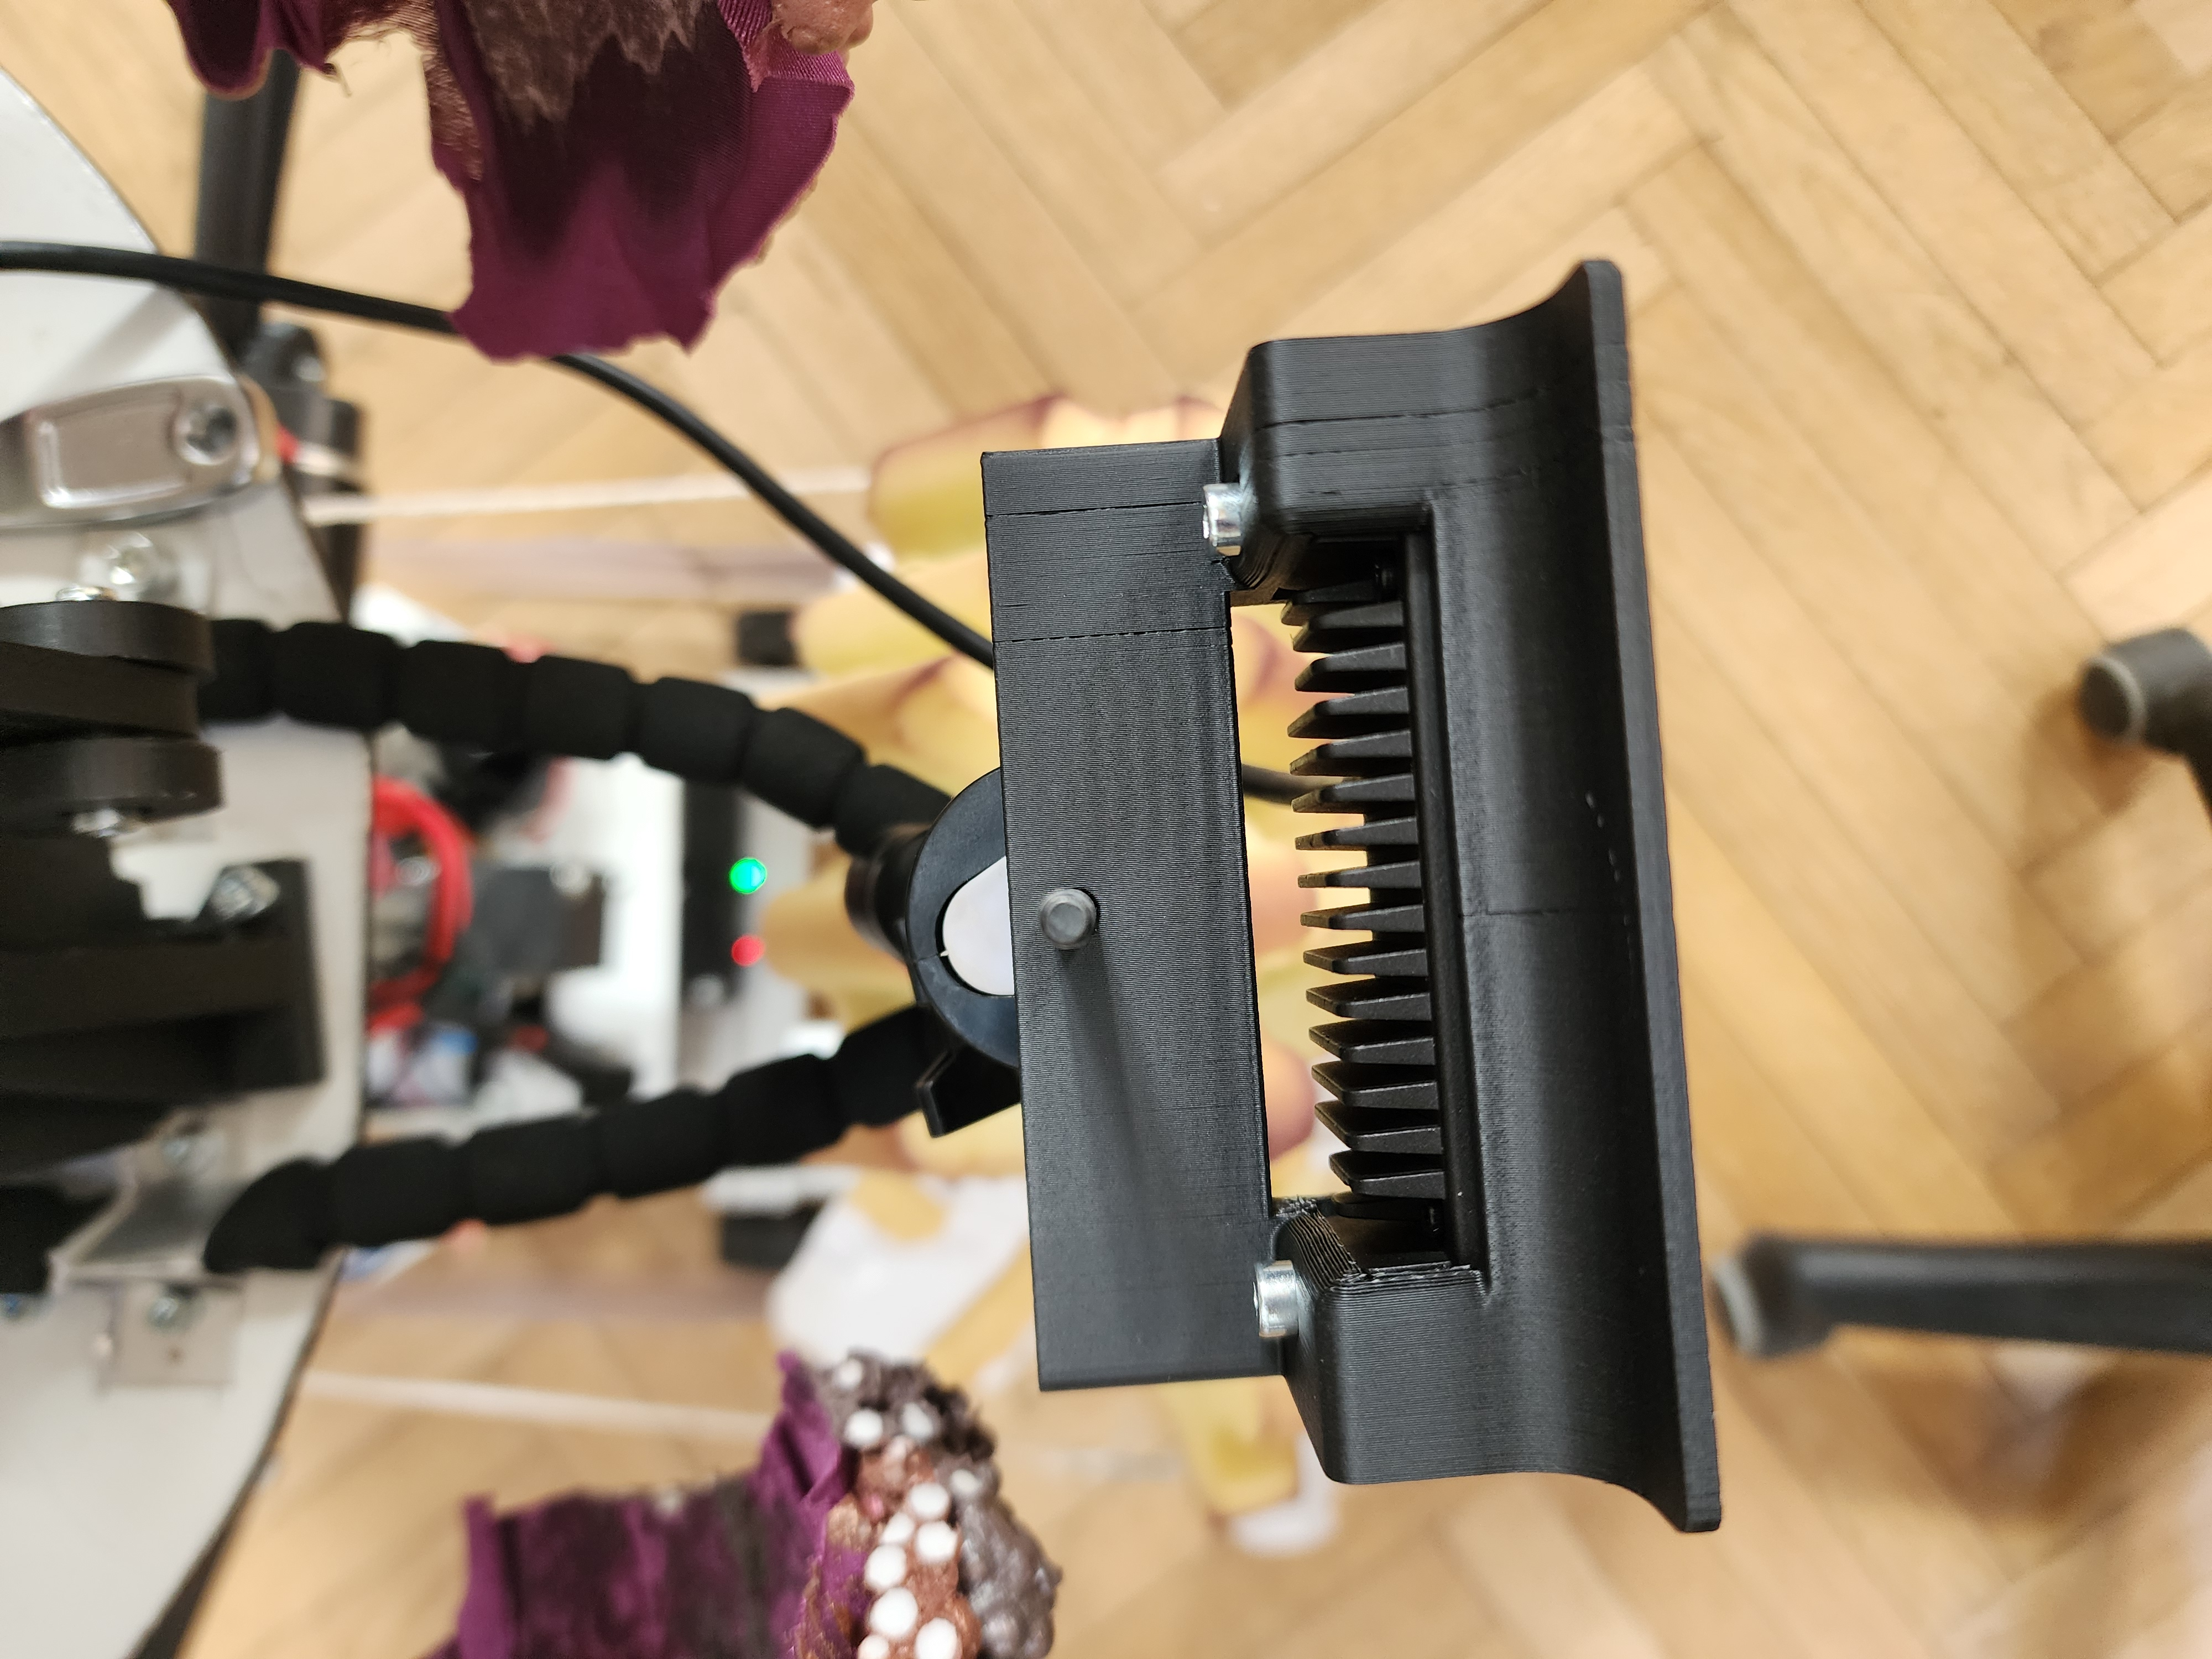
\includegraphics[width=\textwidth, angle=-90]{Images/CameraCasingNoMesh (3).jpg}
        \caption{Camera Casing without Mesh Covering (Top View)}
        \label{fig:camera_casing_no_mesh_top}
    \end{minipage}
\end{figure}

\subsubsection{Velcro Fabric Control System}

The fabric control system utilizes velcro attachments integrated with shell flaps to provide positive fabric positioning control. Flap design provides secure attachment points while maintaining fabric flexibility during robot movement.

Velcro implementation includes both shell-mounted components and fabric-sewn counterparts that provide reliable attachment while enabling fabric removal for maintenance. Attachment strength optimization provides secure positioning without excessive fabric stress.

Field testing validates velcro system effectiveness during extended operational periods including various robot movements and interaction scenarios. Testing confirms reliable fabric positioning without attachment failure or fabric damage.

\subsection{Optical Performance Optimization}

The camera integration system maintains optimal optical performance while addressing the unique challenges of fabric-integrated sensing systems.

\subsubsection{Field of View Protection and Optimization}

Field of view protection strategies ensure consistent camera visibility throughout robot operational ranges while accommodating fabric movement and positioning variations. Protection effectiveness validation includes testing under various lighting conditions and robot orientations.

Mesh covering implementation conceals camera presence from casual observation while maintaining full optical transmission characteristics. Mesh selection balances concealment effectiveness against optical performance impact, ensuring minimal image quality degradation.

Optical testing validates maintained image quality and depth sensing performance through the concealment system. Testing includes calibration verification and performance comparison against uncovered camera operation to ensure minimal performance impact.

\subsubsection{Heat Management and Sustained Operation}

Heat dissipation optimization addresses the Oak-D Pro camera's thermal requirements during sustained operation, particularly during high computational load scenarios including simultaneous SLAM processing and human detection.

Cooling system design utilizes strategic airflow management that enables heat dissipation while maintaining environmental protection. Thermal testing validates sustained operation capability under maximum computational loads without thermal throttling.

\section{Audio System Integration}

The audio system integration enables comprehensive bidirectional communication capabilities for VR integration and enhanced human-robot interaction through carefully designed hardware implementation and dynamic audio processing.

\subsection{Hardware Component Selection and Specifications}

The audio hardware selection prioritizes high-quality bidirectional communication capability while maintaining integration compatibility with Tino's existing system architecture and space constraints.

\subsubsection{iTalk-01 Omnidirectional Microphone Integration}

The iTalk-01 omnidirectional microphone provides 360-degree audio capture capability suitable for social robot interaction scenarios where human positioning relative to the robot varies continuously. Microphone specification analysis demonstrates adequate sensitivity and frequency response for speech capture and environmental audio monitoring.

Mounting considerations address the unique challenges of integrating audio capture equipment within Tino's fabric head structure while maintaining acoustic performance and physical protection. Microphone positioning optimization balances audio quality against mechanical protection and aesthetic integration requirements.

Fabric integration methodology enables microphone mounting through strategic fabric modifications that provide audio access without compromising Tino's visual appearance. Integration techniques utilize fabric properties to provide acoustic coupling while maintaining environmental protection for sensitive electronic components.

\subsubsection{Speaker System Selection and Placement}

The speaker system selection prioritizes clear audio reproduction capability within the geometric and weight constraints of Tino's head assembly. Speaker placement within the servo head maximizes available space utilization while providing optimal acoustic coupling for human interaction scenarios.

Acoustic performance optimization addresses the challenges of speaker operation within a constrained and partially enclosed environment. Speaker mounting utilizes available space within the servo head structure while ensuring adequate acoustic coupling and preventing mechanical interference with head movement systems.

Integration with existing head systems ensures speaker mounting does not interfere with Stewart platform operation, camera mounting, or other head-mounted systems. Geometric optimization provides secure speaker mounting while maintaining system accessibility for maintenance and adjustment.
\begin{figure}[H]
    \centering
    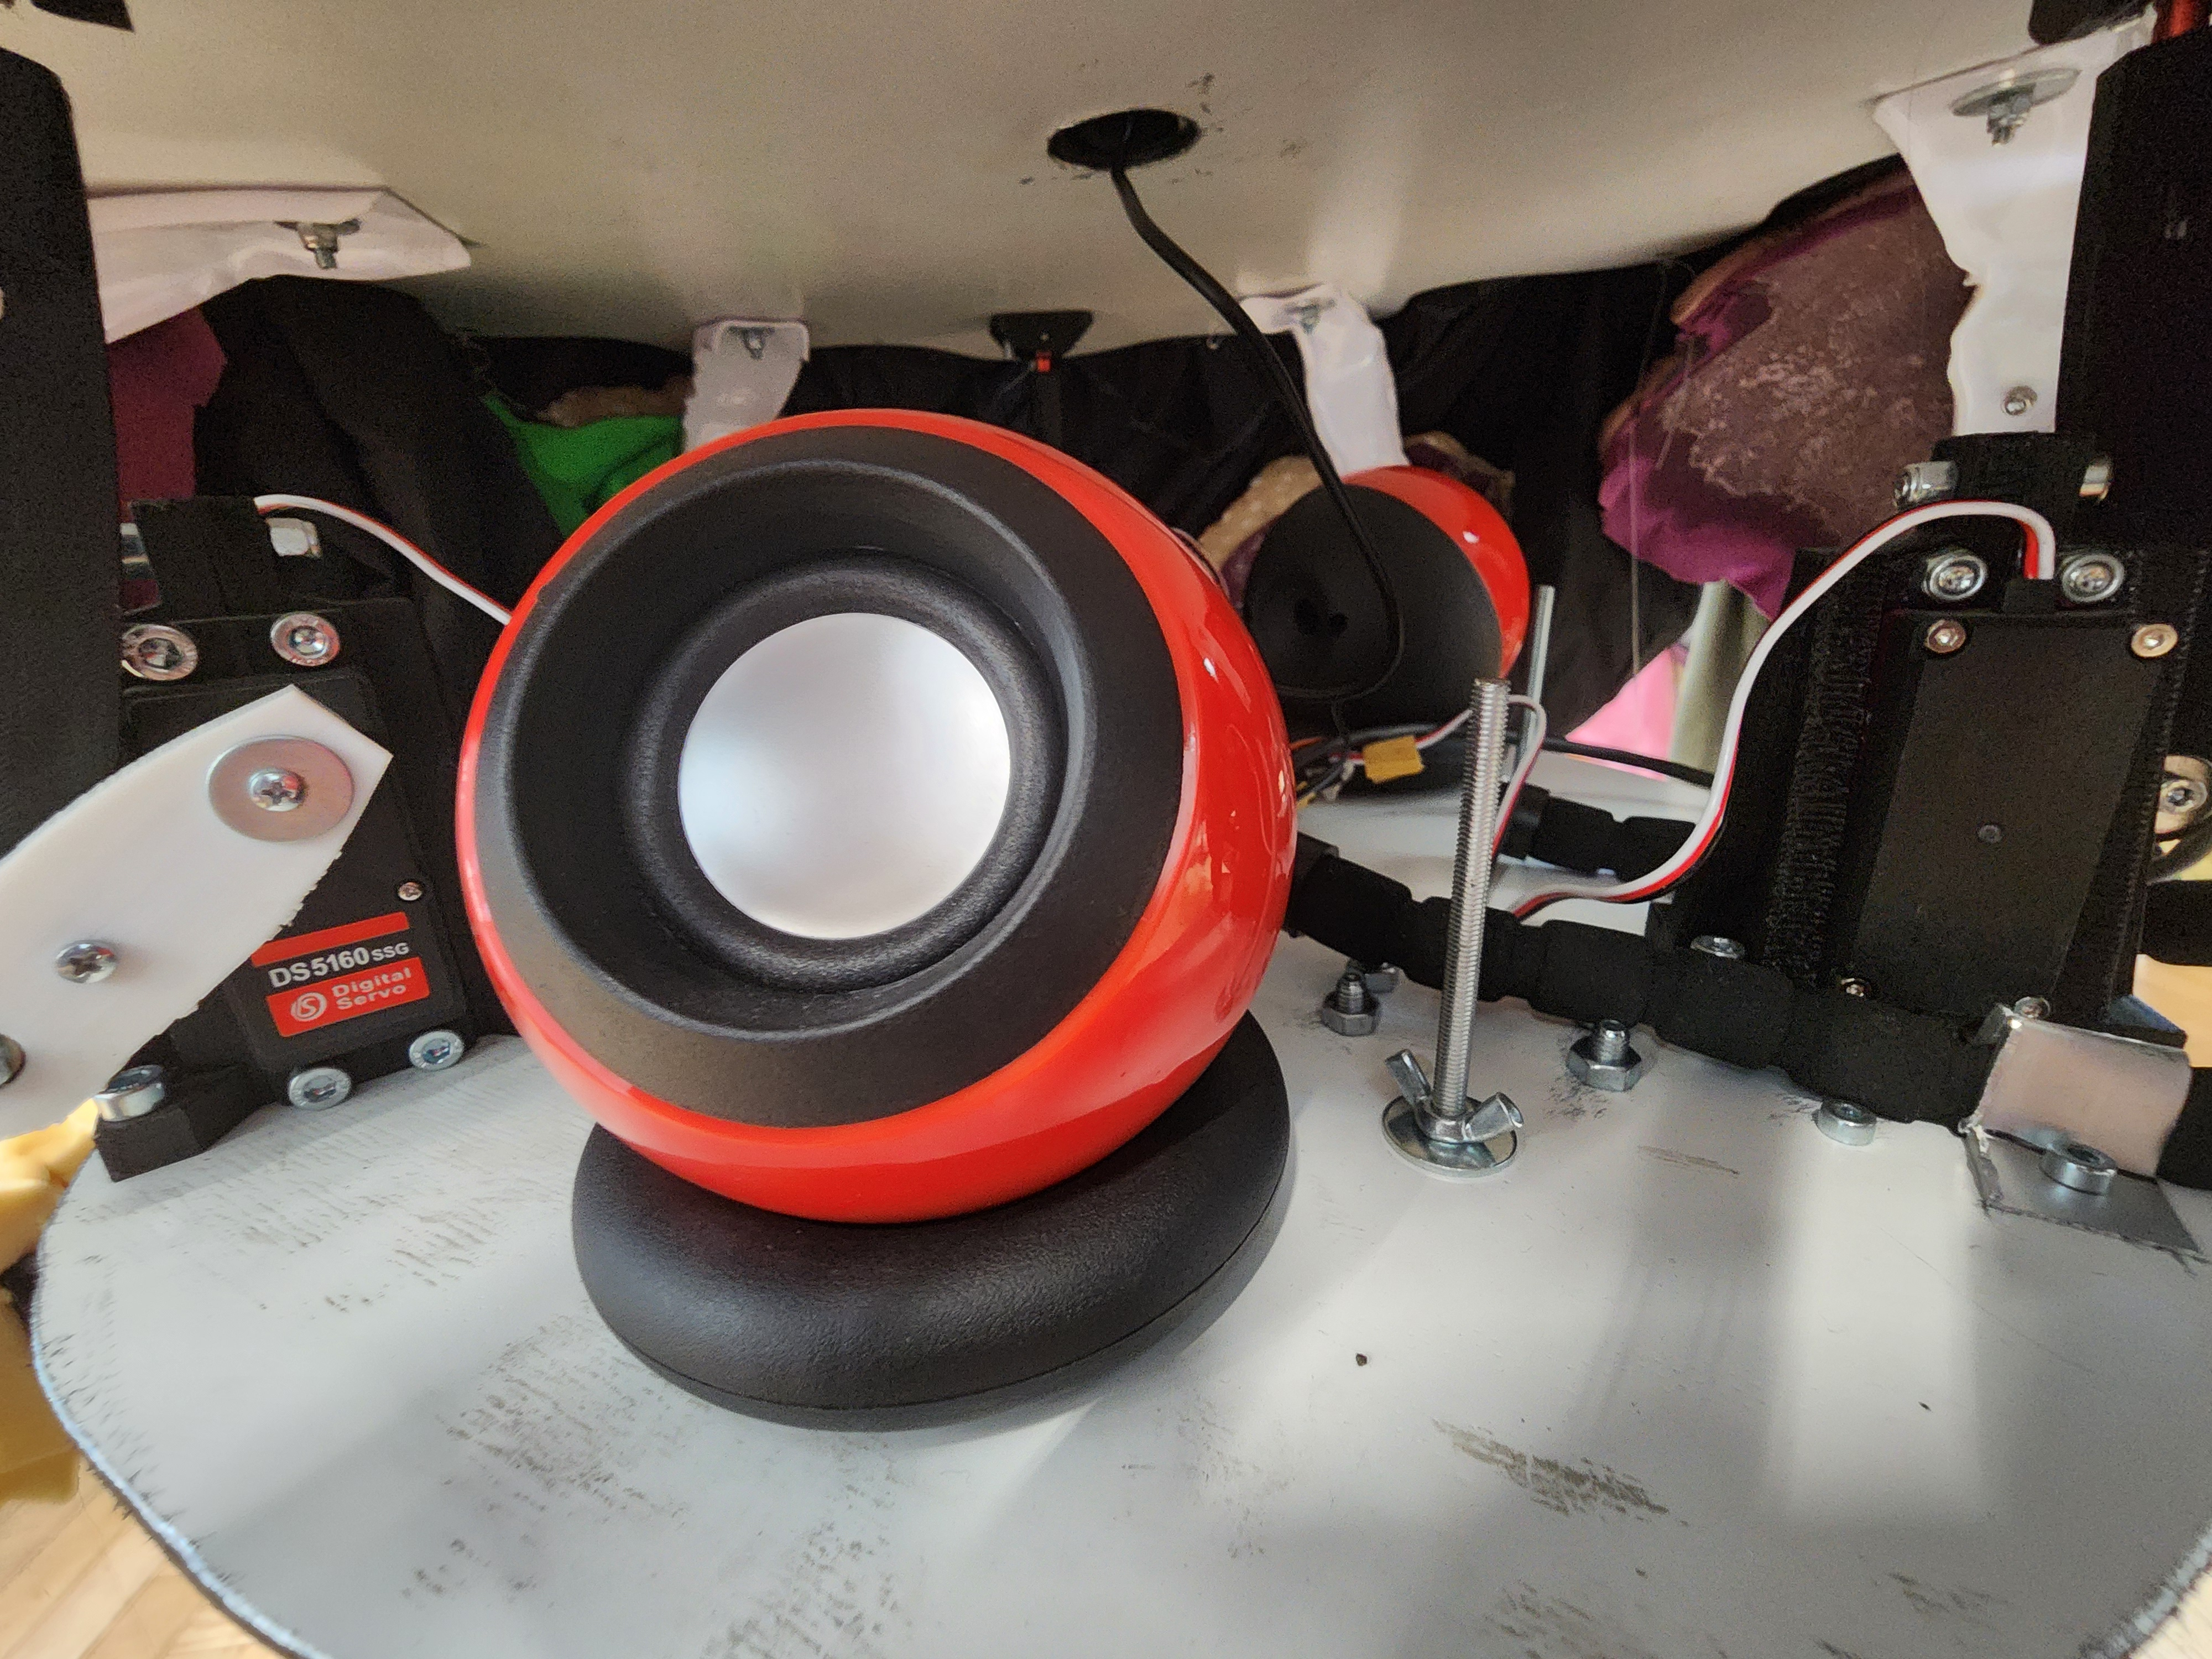
\includegraphics[height=6cm]{Images/SpeakerSetup (2).jpg}
    \caption{Speaker Mounted within Servo Head Structure}
    \label{fig:speaker_mount}
\end{figure}

\subsection{Dynamic Audio Generation and Custom Sound Design}

The audio system implements sophisticated sound generation capabilities that create custom ambient audio specifically designed for Tino's character expression and VR integration requirements.

\subsubsection{No-Face Inspired Audio Algorithm}

The dynamic audio generation utilizes a complex algorithm inspired by the No-Face character from Studio Ghibli films, creating an eerie and mysterious ambient sound that enhances Tino's social presence. The \texttt{noface\_params} system maintains breathing phase control, breath cycle management, and dynamic volume adjustment to create organic, living audio characteristics.

The breathing simulation algorithm implements a state machine with inhale and exhale phases, utilizing sinusoidal wave patterns with randomized duration (2.5-4.0 seconds) and volume variations (0.55-0.75 amplitude range) to create natural breathing rhythm variations. The system maintains continuous audio output while avoiding mechanical repetition through breath parameter randomization.

Multi-tone synthesis combines three base frequencies (110Hz, 146.83Hz, 73.42Hz) with pre-calculated gain values (0.65, 0.45, 0.25) to create rich harmonic content. Filtered breath noise generation utilizes a first-order low-pass filter (coefficient 0.92) applied to random noise, creating organic texture that varies with breathing intensity.

The audio generation operates at 44.1kHz sample rate with 1024-sample chunks, ensuring high-quality audio output while maintaining real-time performance compatibility with other system components including SLAM processing and human detection.

\subsubsection{Real-Time Audio Parameter Control}

The audio control system receives real-time parameters from the VR interface through ROS2 topics, enabling dynamic audio modification based on user interaction and robot state. The \texttt{vr\_audio\_callback} function processes \texttt{Float32MultiArray} messages containing volume (0-255 range) and orientation (-1.0 to 1.0 range) control values.

Volume control implementation applies logarithmic scaling to provide natural perceived loudness variations while maintaining system audio output limits. The volume parameter directly scales the final audio amplitude, enabling seamless integration with VR-controlled audio levels based on proximity and interaction intensity.

Orientation-based parameter modulation enables frequency shifting and audio characteristic changes based on spatial positioning. The orientation parameter influences base frequency modulation (±20\% frequency variation) and breathing pattern intensity, creating spatial audio awareness that enhances immersive VR interaction.

\subsection{Stereo Speaker Configuration and Spatial Audio Processing}

The stereo speaker system provides sophisticated spatial audio capabilities through advanced panning algorithms and stereo field manipulation optimized for social robot interaction scenarios.

\subsubsection{Enhanced Stereo Panning Implementation}

The stereo panning system implements aggressive channel separation techniques that create dramatic spatial audio effects controlled by VR input orientation values. The panning algorithm utilizes non-linear curves with exponential falloff characteristics to provide pronounced left-right audio separation that enhances directional audio expression.

Channel separation calculations apply quadratic intensity scaling where \texttt{pan\_intensity = min(1.0, abs(orientation) * 1.5)} creates exponential panning response curves. Right-side dominance utilizes \texttt{left\_vol = volume\_scale * (1.0 - (orientation\_effect * 1.1 + pan\_intensity\^2 * 0.5))} while left-side dominance applies equivalent mirrored calculations for balanced spatial control.

Channel boost implementation provides 30\% amplitude enhancement on the dominant channel (\texttt{right\_vol = volume\_scale * (1.0 + orientation\_effect * 0.3)}) while applying aggressive attenuation up to 95\% on the opposite channel. This creates pronounced stereo separation that maintains 5\% minimum volume to prevent complete channel silence.

The panning system maintains real-time responsiveness with orientation updates processed at audio sample rate, enabling smooth spatial transitions that follow VR user head movements without audible artifacts or discontinuities.

\subsubsection{Audio Expression and Robot Personality Integration}

The stereo audio system enhances Tino's expressive capabilities by correlating spatial audio characteristics with robot emotional states and interaction contexts. Spatial audio positioning creates directional personality expression where left-right audio bias suggests attention direction and emotional focus.

Breathing pattern modulation integrates with stereo positioning to create complex audio landscapes where breath intensity, frequency content, and spatial positioning combine to express robot internal states. The system maintains acoustic coherence while providing rich expressive variation through multi-dimensional audio parameter control.

VR integration enables precise control over robot audio personality through real-time parameter adjustment, allowing users to influence robot audio expression through spatial positioning, proximity, and interaction intensity. This creates responsive audio feedback that enhances social presence and interaction naturalness.

\section{YOLOv11 Pose Detection Implementation with TensorRT Optimization}

The YOLOv11 pose detection system provides real-time human skeleton tracking capabilities optimized for the NVIDIA Orin Nano platform through advanced TensorRT acceleration and efficient model deployment strategies.

\subsection{YOLOv11 Architecture Selection and Model Optimization}

The YOLOv11 architecture selection prioritizes the balance between detection accuracy and computational efficiency required for real-time embedded operation on the Orin Nano platform.

\subsubsection{YOLOv11n-Pose Model Selection}

The \texttt{yolo11n-pose.pt} model provides optimal performance characteristics for the Orin Nano's computational constraints while maintaining adequate accuracy for social robot interaction requirements. The nano variant (11n) utilizes a streamlined architecture with reduced parameter count compared to larger YOLO variants, enabling real-time inference on embedded hardware.

Model architecture analysis demonstrates the YOLOv11n-pose network's capability to detect multiple humans simultaneously within the camera's field of view while maintaining frame rates suitable for interactive applications. The model's optimized backbone reduces computational overhead while preserving essential feature detection capabilities for robust human pose estimation.

Pre-trained model utilization eliminates extensive training requirements by leveraging weights trained on large-scale pose estimation datasets. The pre-trained approach provides immediate deployment capability while ensuring robust performance across diverse human poses and environmental conditions typical of social robot applications.

\subsubsection{Model Format Conversion Pipeline}

The model optimization pipeline transforms the original PyTorch format through multiple conversion stages to achieve maximum performance on the target hardware. The conversion process begins with the native \texttt{.pt} PyTorch format and progresses through ONNX and TensorRT formats for optimal deployment.

ONNX format conversion (\texttt{.onnx}) provides cross-platform compatibility and serves as an intermediate representation that enables hardware-specific optimizations. The ONNX conversion maintains model accuracy while enabling subsequent optimization passes that target the Orin Nano's specific GPU architecture.

TensorRT engine generation (\texttt{.engine}) represents the final optimization stage, creating hardware-specific inference engines that maximize GPU utilization on the Orin Nano platform. The TensorRT optimization process includes layer fusion, precision calibration, and memory access optimization that significantly improve inference performance compared to standard deployment methods.

\subsection{TensorRT Engine Optimization Process}

The TensorRT optimization process generates highly efficient inference engines specifically optimized for the Orin Nano's GPU architecture and memory hierarchy.

\subsubsection{Engine Generation and Hardware Optimization}

TensorRT engine generation utilizes the Orin Nano's specific GPU capabilities to optimize network execution through layer fusion, kernel optimization, and memory access pattern optimization. The process analyzes the YOLOv11n-pose network structure and generates optimized CUDA kernels that maximize throughput while minimizing memory bandwidth requirements.

Precision optimization techniques evaluate the network's sensitivity to reduced precision arithmetic, enabling mixed-precision computation that balances accuracy against performance. The optimization process may utilize INT8 quantization where appropriate while maintaining FP16 or FP32 precision for critical network layers that require higher numerical accuracy.

Memory allocation strategies optimize GPU memory usage patterns to prevent memory fragmentation and minimize allocation overhead during inference operations. The TensorRT engine pre-allocates memory buffers and optimizes data transfer patterns between CPU and GPU memory to minimize inference latency.

\subsubsection{Performance Profiling and Validation}

Engine performance validation ensures that TensorRT optimizations maintain pose detection accuracy while achieving target inference rates. Performance profiling includes accuracy benchmarking against the original PyTorch model to verify that optimization processes do not compromise detection quality.

Throughput analysis measures inference performance under various loading conditions including single and multi-person detection scenarios. Performance metrics include inference latency, GPU utilization, and memory bandwidth utilization that validate the engine's suitability for real-time social robot applications.

Thermal analysis ensures that sustained inference operations remain within the Orin Nano's thermal limits during extended operation periods. Thermal validation includes continuous operation testing under maximum computational loads to ensure system stability and reliability.

\subsection{ROS2 Node Architecture and Integration}

The pose detection system integrates seamlessly with Tino's ROS2 architecture through a dedicated node that manages camera input, inference execution, and result publication.

\subsubsection{Camera Topic Subscription and Data Flow}

The \texttt{pose\_detection\_node.py} subscribes to Oak-D Pro camera topics including \texttt{/right/image\_rect} for monocular RGB input and \texttt{/stereo/depth} for corresponding depth information required for 3D coordinate calculation. The node implements efficient message handling with \texttt{CvBridge} conversion from ROS2 image messages to OpenCV format suitable for YOLO processing.

Image preprocessing includes monocular to BGR conversion for YOLO compatibility, since the implementation uses the right camera feed converted from mono8 to BGR format. The preprocessing pipeline utilizes CPU-based OpenCV operations for format conversion while maintaining real-time performance through efficient memory management.

Synchronization mechanisms maintain temporal alignment between RGB and depth image streams through callback-based processing that ensures corresponding depth information is available for each processed RGB frame. The implementation uses a latest-frame approach where \texttt{latest\_image} and \texttt{latest\_depth\_image} are synchronized for pose detection processing.

\subsubsection{Inference Execution and Result Processing}

TensorRT inference execution utilizes the pre-converted \texttt{yolo11n-pose.engine} model loaded from the package resource directory through \texttt{YOLO (model\_path)} initialization. The inference pipeline processes BGR images directly with configurable confidence thresholding (default 0.5) and \texttt{verbose=False} parameter to suppress detection logging output.

Result post-processing extracts pose keypoints, confidence scores, and bounding box information from the \texttt{results[0]} object returned by YOLO inference. Post-processing operations include confidence-based filtering, closest person selection based on depth measurements, and coordinate extraction from the \texttt{results[0].boxes} and \texttt{results[0].keypoints} attributes.

Error handling implements comprehensive exception management with detailed logging at configurable levels (INFO, DEBUG, ERROR) and graceful degradation when model loading fails or inference encounters errors. The system maintains operational continuity through try-catch blocks around critical processing sections.

\section{Stereo Depth Integration for 3D Human Positioning}

The stereo depth integration system combines 2D pose detection results with Oak-D Pro depth information to provide accurate 3D human positioning capabilities essential for spatial awareness and interaction planning.

\subsection{Oak-D Pro Depth Data Utilization}

The Oak-D Pro camera system provides synchronized stereo depth information that enables precise 3D coordinate calculation for detected human pose keypoints.

\subsubsection{Stereo Depth Acquisition and Processing}

The Oak-D Pro stereo camera system generates depth maps through stereo vision algorithms that calculate depth values for each pixel in the synchronized color image. Depth data accuracy depends on stereo baseline, camera calibration quality, and environmental factors including lighting conditions and surface textures.

Depth value extraction utilizes a median-based approach with a 9x9 pixel window around keypoint locations to obtain robust depth measurements. The \texttt{get\_depth\_at\_point} function implements outlier filtering by calculating median and standard deviation, then filtering values more than 2 standard deviations from the median to ensure reliable depth extraction.

Depth data validation implements comprehensive quality filtering including zero-value rejection, outlier detection based on statistical analysis, and temporal smoothing over a configurable window size (default 3 frames). The validation process uses median filtering within pixel windows and consistency checks against reference depth values to maintain measurement reliability.

For person detection, the system uses \texttt{get\_median\_depth} function that extracts depth from a central region of the bounding box with configurable padding (25\% by default), providing more stable depth measurements than single-pixel sampling while avoiding background contamination.

\subsubsection{Coordinate System Transformation}

Camera frame to robot coordinate transformation converts 3D keypoint coordinates using the \texttt{calculate\_3d\_position} function that utilizes camera intrinsic parameters from \texttt{camera\_info.k} array. The transformation extracts focal lengths \texttt{fx}, \texttt{fy} and principal point coordinates \texttt{cx}, \texttt{cy} from the camera calibration matrix.

Intrinsic parameter utilization includes automatic unit conversion detection where depth values greater than 100 are converted from millimeters to meters, followed by depth calibration correction using configurable \texttt{depth\_scale\_factor} (default 0.575) and \texttt{depth\_offset} parameters derived from empirical calibration measurements.

3D coordinate calculation applies the standard pinhole camera model: \texttt{x\_3d = (x - cx) * z / fx} and \texttt{y\_3d = (y - cy) * z / fy}, where corrected depth \texttt{z = z * depth\_scale\_factor + depth\_offset} accounts for systematic depth measurement biases in the Oak-D Pro stereo system.

\subsection{3D Skeleton Generation and Validation}

The 3D skeleton generation process combines 2D keypoint detections with corresponding depth values to create complete 3D human pose representations.

\subsubsection{Keypoint Depth Association}

Depth value assignment utilizes the 2D keypoint pixel coordinates to extract corresponding depth measurements from the stereo depth map. The assignment process includes validation to ensure depth measurements correspond to human body parts rather than background objects.

Depth consistency validation utilizes a sophisticated temporal smoothing system where individual keypoint depths are validated against a reference depth calculated as the median of all valid keypoint depths. The \texttt{process\_skeleton} function implements outlier rejection where keypoint depths deviating more than the configurable \texttt{depth\_outlier\_threshold} (default 30\%) from the reference are replaced with the temporal median depth from a smoothing window.

Missing depth handling addresses invalid keypoint scenarios through the reference depth fallback system. When keypoint coordinates are marked as invalid ($x \leq 0$ or $y \leq 0$) or depth extraction fails, the system utilizes the temporally smoothed reference depth calculated from all valid keypoints in the current frame, ensuring skeleton completeness even with partial occlusion.

The temporal smoothing implementation maintains a \texttt{skeleton\_depth\_history} list with configurable window size (default 3 frames) that stores reference depths for median filtering over time, providing stable depth values that reduce measurement jitter while maintaining responsiveness to actual depth changes.

\subsection{Real-time Processing and Performance Optimization}

The 3D positioning system maintains real-time performance while processing high-resolution depth data and performing complex coordinate transformations.



\section{Real-time Skeleton Tracking with 17 Key Body Joints}

The skeleton tracking system processes YOLOv11 pose detection results to extract and organize 17 standard COCO keypoints into structured human pose representations suitable for social robot interaction analysis.

\subsection{COCO Keypoint Framework Implementation}

The COCO keypoint framework provides a standardized representation for human pose detection that ensures compatibility with established computer vision tools and datasets.

\subsubsection{17-Keypoint Detection Schema}

The YOLOv11 pose detection system identifies 17 key body joints following the COCO pose estimation standard: nose (0), left eye (1), right eye (2), left ear (3), right ear (4), left shoulder (5), right shoulder (6), left elbow (7), right elbow (8), left wrist (9), right wrist (10), left hip (11), right hip (12), left knee (13), right knee (14), left ankle (15), and right ankle (16).

Joint indexing follows the established COCO convention ensuring compatibility with existing pose analysis tools and datasets. The consistent indexing scheme enables straightforward integration with pose analysis algorithms and facilitates comparison with other human pose detection systems.

Keypoint connectivity defines the skeletal structure through predefined joint relationships that represent human anatomical connections. The connectivity graph includes head structure (nose-eyes-ears), torso connections (shoulders-hips), and limb chains (shoulder-elbow-wrist, hip-knee-ankle) that enable skeletal validation and pose completeness assessment.

\subsubsection{Confidence Scoring and Quality Assessment}

Confidence score extraction provides reliability metrics for each detected keypoint, enabling quality-based filtering and uncertainty quantification. Confidence values range from 0.0 (undetected) to 1.0 (high confidence) and indicate the detection algorithm's certainty in keypoint localization accuracy.

Quality thresholding implements confidence-based filtering that excludes low-confidence detections from downstream processing. Threshold values balance detection completeness against accuracy requirements, with typical thresholds ranging from 0.3 to 0.7 depending on application requirements and environmental conditions.

Multi-person confidence handling manages confidence scores when multiple humans are detected simultaneously. The system maintains separate confidence profiles for each detected person while implementing consistency checks that ensure skeletal coherence within individual pose detections.

\subsection{Data Processing Pipeline and Skeleton Organization}

The data processing pipeline transforms raw YOLOv11 output into structured skeleton representations suitable for real-time robot applications.

\subsubsection{Keypoint Coordinate Extraction}

Raw network output processing extracts keypoint coordinates and confidence scores from YOLOv11 inference results. The extraction process handles variable-length outputs that accommodate different numbers of detected humans while maintaining consistent data structures for downstream processing.

Coordinate normalization converts pixel coordinates to standardized coordinate systems that enable consistent processing regardless of camera resolution or field of view variations. Normalization includes scaling, translation, and coordinate system alignment that simplifies subsequent geometric calculations.

\subsubsection{Skeleton Structure Validation}

Geometric consistency validation implements anatomical constraints that verify reasonable joint relationships within detected skeletons. Validation includes bone length checks, joint angle limitations, and bilateral symmetry assessments that identify and filter implausible pose detections.

Temporal consistency analysis compares consecutive pose detections to identify and smooth measurement noise while detecting rapid pose changes that indicate genuine human motion. Temporal filtering balances noise reduction against motion tracking accuracy to maintain responsive pose tracking.

Completeness assessment evaluates skeleton quality based on the number and distribution of successfully detected keypoints. Assessment criteria include minimum keypoint requirements, critical joint detection (head, torso, limbs), and pose coverage metrics that indicate skeleton suitability for specific applications.

\subsection{ROS2 Message Publishing and Data Distribution}

The skeleton tracking system publishes pose data through ROS2 topics enabling integration with other robot systems and applications.

\subsubsection{Custom Message Structure Design}

ROS2 message design implements multiple specialized publishers for different data requirements: \texttt{/pose\_detection/image\_raw} for annotated detection images, \texttt{/human\_position} for smoothed human position using \texttt{PoseStamped} messages, \texttt{/human\_skeleton} for 3D skeleton visualization using \texttt{MarkerArray}, and \texttt{/human\_skeleton\_poses} for programmatic access to joint coordinates using \texttt{PoseArray} messages.

Multi-person message handling focuses on closest person selection based on depth measurements, where the system identifies the person with minimum depth value and processes only that individual's skeleton data. This approach reduces computational overhead while ensuring consistent tracking of the most relevant human for interaction applications.

Timestamp synchronization utilizes \texttt{self.get\_clock ().now ().to\_msg ()} for all published messages with consistent \texttt{header.frame\_id} set to the configurable camera frame (default: \texttt{oak\_right\_camera\_optical\_frame}), ensuring temporal alignment across all pose-related data streams.

\subsection{Integration with Robot Controller and VR Systems}

Skeleton data integration enables sophisticated human-robot interaction capabilities through real-time pose information distribution to various robot subsystems.

\subsubsection{Robot Controller Integration}

The robot controller subscribes to \texttt{/human\_position} topic for spatial awareness applications where human position data undergoes temporal smoothing through the \texttt{publish\_human\_position} function. This implementation maintains a configurable history buffer (default 5 positions) and publishes averaged coordinates to reduce measurement jitter while maintaining responsiveness to human movement.

Pose-based behavior triggers can utilize the multiple data streams including raw skeleton data from \texttt{/human\_skeleton\_poses} for detailed joint analysis, smoothed position data from \texttt{/human\_position} for proximity detection, and visual markers from \texttt{/human\_skeleton} for debugging and visualization purposes.

Safety monitoring implementation prioritizes closest person detection where the system automatically selects the human with minimum depth measurement for tracking, ensuring safety systems focus on the most immediate interaction partner while maintaining computational efficiency through single-person processing.

\subsubsection{VR Data Recording and Transmission}

VR system integration transmits skeleton data for immersive visualization and interaction analysis applications. Integration includes data formatting for Unity applications and network transmission protocols optimized for VR system requirements.

Data recording capabilities capture complete skeleton tracking sessions for offline analysis and system evaluation. Recording includes synchronized pose data, camera images, and robot state information that enable comprehensive interaction analysis and system performance assessment.

Bandwidth optimization implements data compression and selective transmission strategies that maintain VR system responsiveness while minimizing network overhead. Optimization techniques include keyframe detection, delta encoding, and adaptive quality adjustment based on network conditions and VR application requirements.


\section{VR System Architecture and Unity Communication}

The VR integration system enables immersive remote control of Tino through Unity-based VR environments via a bidirectional UDP communication protocol that maintains real-time responsiveness while providing comprehensive robot state information.

\subsection{VR Interface Node Architecture}

The \texttt{vr\_interface\_node.py} serves as the central communication bridge between Tino's ROS2 ecosystem and Unity VR applications. The node subscribes to robot pose data (\texttt{/vr\_in/robot\_pose}), human skeleton information (\texttt{/vr\_in/human\_skeleton\_poses}), and audio output (\texttt{/vr\_in/audio\_output}), while publishing VR control commands to \texttt{/vr\_out/cmd\_vel} for base movement and \texttt{/vr\_out/head\_cmd} for head articulation.

The multi-threaded architecture utilizes dedicated UDP listener threads with 1-second timeouts for non-blocking message reception while enabling simultaneous outgoing data transmission. Error handling includes automatic VR disconnection detection (3-second timeout) and message ordering counter reset upon reconnection.

\subsection{UDP Communication Protocol}

The protocol implements a three-port architecture for parallel data streams: port 5005 receives 32-byte VR command packets, port 5006 transmits 24-byte robot pose data, and port 5007 streams 208-byte skeleton data containing 17 COCO-format joints.

Incoming command packets contain 3 floats for head control (pitch, pan, tilt), 2 integers for base commands (state 0-3, angular direction -1/0/1), 2 values for audio control (volume 0-255, orientation -1.0 to 1.0), and 1 integer for message ordering. Binary encoding uses \texttt{struct.unpack('fffiiffi', data)} with validation for length verification and parameter range checking.

Outgoing pose packets include message ordering, position coordinates (x, y), orientation quaternion (z, w), and audio volume, optimized for 10Hz transmission rates. Message ordering counters enable detection of lost, duplicate, or out-of-order packets with automatic counter reset during reconnection events.

\section{Atomic Movement System Design and 4-State Control Architecture}

The atomic movement system replaces traditional continuous control with discrete, completion-guaranteed movements ensuring perfect correspondence between VR user intentions and physical robot actions. The unified 4-state framework provides standardized behavior across both leg and base controllers.

\subsection{4-State Control Framework}

\subsubsection{State 0: Idle and Auto-Positioning}

State 0 maintains neutral configurations with intelligent auto-positioning for the leg controller. The system uses absolute encoder feedback to calculate position differences from neutral (0 ticks) and applies appropriate motor commands: 110 RPM forward when negative position, 70 RPM backward when positive, and 90 RPM neutral when within 50 ticks. The base controller implements complete motion cessation with flag reset.

\subsubsection{State 1: Expressive ``Little Push'' Movements}

State 1 implements attention-getting behaviors. The leg controller uses an optimized 3-phase pattern: 50\% forward extension, 5\% pause, 45\% return over 1.2 seconds via the \texttt{vtLittlePush()} function. The base controller executes a 600ms delay, 200ms forward, 200ms backward sequence for directional indication.

\subsubsection{State 2: Timing Synchronization}

State 2 enables coordinated multi-component movements. The leg controller extends to maximum reach using \texttt{vtForwardOnly()} then activates position hold mode with PID control (Kp=2.0, Ki=0.1, Kd=0.5). The base controller implements a 1.5-second timing cycle with command queuing for received case 3 commands.

\subsubsection{State 3: Atomic Movement Execution}

State 3 executes completion-guaranteed operations. The leg controller returns to neutral using home button detection as completion criteria. The base controller provides three movement types: forward (angular=0), right rotation (angular=1), left rotation (angular=-1), each with 1.7-second duration.

\subsection{Implementation Details}

The leg controller maintains absolute position through encoder integration with direction-specific scaling (forward 1.15, backward 0.85) and automatic reset on button press. The base controller uses \texttt{updateBaseMovementByTime()} with millisecond-precision timing and sophisticated locking mechanisms (\texttt{isCase2Locked}) that coordinate execution between components.

\section{Pulse-Based Command System for VR Integration}

The pulse-based command architecture replaces continuous signal transmission with discrete 3-cycle command pulses that automatically return to idle state, ensuring each VR interaction triggers exactly one complete robot movement cycle.

\subsection{Command Pulse Structure}

Each user action generates three identical command cycles followed by automatic return to idle (command 0). Pulse timing uses 40ms intervals between transmissions (120ms total duration) to exceed network latency variations while preventing command accumulation. The 3-cycle repetition ensures reliable delivery across network interruptions with command validation through parameter consistency checking.

VR input processing transforms continuous actions into discrete events through rising-edge triggering on button activation, preventing continuous command generation during extended holds. Input debouncing requires 200ms minimum intervals between commands while encoding current VR state (head orientation) at command initiation time.

\subsection{Gamepad Development Integration}

Gamepad control mirrors VR functionality using discrete button commands: X (state 1), Y (state 2), B (state 3), A (idle). Shoulder buttons enable combined movement testing with simultaneous angular direction commands. The identical pulse generation system ensures development testing accurately represents VR operational behavior.

\subsection{VR Command Processing}

UDP packet processing extracts commands from 32-byte binary structures using \texttt{struct.unpack('fffiiffi', data)} format. Head commands (pitch, pan, tilt) forward directly to robot controllers, while base commands (state 0-3, angular -1/0/1) trigger atomic movement execution. Message ordering uses 32-bit sequence numbers for duplicate detection and lost packet monitoring, with automatic counter reset during VR reconnection events.

\section{Unity-ROS2 Communication Protocol and Message Structures}

The Unity-ROS2 communication protocol implements optimized UDP-based data exchange designed for real-time VR applications with robust reliability and comprehensive monitoring capabilities.

\subsection{Multi-Port UDP Architecture}

The system uses three dedicated ports for parallel data streams: port 5005 (VR commands, 32-byte packets), port 5006 (robot pose, 24-byte packets), and port 5007 (skeleton data, 208-byte packets). This isolation prevents interference while enabling independent optimization for different data types and latency requirements.

Network configuration supports flexible deployment through configurable IP addresses and transmission rates. Default settings target address 192.168.0.201 with pose/skeleton transmission at 10Hz and expected command reception at 25Hz.

\subsection{Message Format Specifications}

Incoming VR commands use a 32-byte binary format: 3 floats (head pitch/pan/tilt), 2 integers (base state 0-3, angular direction -1/0/1), 2 values (audio volume 0-255, orientation -1.0 to 1.0), and 1 integer (message ordering). Binary encoding uses \texttt{struct.unpack('fffiiffi', data)} with comprehensive validation for length, range, and ordering.

Outgoing robot pose packets contain: message ordering, position coordinates (x, y), orientation quaternion (z, w), and audio volume in 24 bytes. Skeleton packets include 51 floats representing 17 COCO joints with default (0,0,0) coordinates for missing joints.

\subsection{Communication Health Monitoring}

The system implements comprehensive monitoring including rate validation against configured targets, connection status tracking with 3-second disconnection timeout, and message ordering validation for duplicate/loss detection. Automatic recovery includes counter reset upon reconnection and detailed diagnostic logging for system maintenance.

\subsection{External Appearance Impact Assessment}

Throughout the comprehensive Tino V2 implementation encompassing ROS2 architecture migration, kinematic base redesign, power system overhaul, Stewart platform improvements, camera integration, and audio system enhancements, the robot's external aesthetic appearance has been deliberately preserved to maintain its distinctive character and proven social interaction capabilities.

The extensive internal modernization—from the fundamental shift to differential drive kinematics and NVIDIA Orin Nano computational platform to the complete redesign of head mechanisms and sensor integration—was strategically executed to operate within Tino's established external form factor. Each upgrade was carefully engineered to enhance technical capabilities while preserving the approachable aesthetic that defines Tino's social robotics effectiveness.

\begin{figure}[H]
    \centering
    \begin{minipage}{0.45\textwidth}
        \centering
        \includegraphics[width=\textwidth, angle=-90]{Images/TinoBefore.jpg}
        \caption{Tino Before V2 Implementation}
        \label{fig:tino_before_upgrade}
    \end{minipage}
    \hfill
    \begin{minipage}{0.45\textwidth}
        \centering
        \includegraphics[width=\textwidth, angle=-90]{Images/FinalTino.jpg}
        \caption{Tino After Complete V2 Upgrade}
        \label{fig:tino_after_upgrade}
    \end{minipage}
\end{figure}

The preservation of Tino's external design language validates the holistic engineering approach that achieved dramatic internal technological advancement while maintaining the established visual identity essential for consistent human-robot interaction research. This balance between comprehensive technical modernization and aesthetic continuity ensures that the V2 platform delivers enhanced capabilities without compromising the social robotics research foundation established by the original design, enabling seamless transition to the upgraded system while maintaining research validity and experimental continuity.
